% !TEX root = FDS_Technical_Reference_Guide.tex

\typeout{new file: Appendices.tex}

\chapter{Nomenclature}
\label{nomenclature}

\begin{tabbing}
$A_{\rm p,c}$ \hspace{1in}\= droplet/particle cross sectional area \\
$A_{\rm p,s}$ \hspace{1in}\= droplet/particle surface area \\
$A_{\alpha\beta}$         \> pre-exponential factor for solid phase Arrhenius reaction \\
B                       \> emission source term; particle mobility \\
$C$                       \> sprinkler C-factor; coefficient of natural convection \\
$C_{\rm d}$               \> drag coefficient \\
$C_{\rm m}$               \> momentum accommodation coefficient \\
Cn                        \> Cunningham slip correction factor \\
$C_{\rm s}$               \> Smagorinsky constant (LES); thermal slip coefficient  \\
$C_{\rm t}$               \> thermal accommodation coefficient \\
$c$                       \> solid material specific heat; speed of light in vacuum \\
$c_p$                     \> constant-pressure specific heat \\
$D$                       \> droplet/particle diameter   \\
$D_{\alpha}$              \> diffusion coefficient \\
$D_{\rm v,0.5}$           \> median volumetric droplet diameter \\
$E$                       \> activation energy \\
Fu                        \> Fuchs factor \\
$\bof_{\rm b}$            \> external force vector (excluding gravity) \\
$g$                       \> acceleration of gravity \\
$\bg$                     \> gravity vector, normally $(0,0,-g)$ \\
$\cH$                      \> total pressure divided by the density (Bernoulli integral)\\
$H_{{\rm r},\alpha\beta}$ \> heat of reaction for a solid phase reaction     \\
$h$                       \> heat transfer coefficient; mass transfer coefficient; enthalpy; Planck constant      \\
$h_{\rm s,\alpha}$        \> sensible enthalpy of species $\alpha$   \\
$I$                       \> radiation intensity per unit of solid angle     \\
$I_{\rm b}$               \> radiation blackbody intensity per unit of solid angle  \\
$I_{b,\rm \la}$           \> spectral radiation blackbody intensity as function of wavelength per unit of solid angle  \\
$I_{b,\rm \om}$           \> spectral radiation blackbody intensity as function of wavenumber per unit of solid angle  \\
$k$                       \> thermal conductivity; suppression decay factor \\
$k_{\rm B}$               \> Boltzmann constant                             \\
Kn                        \> Knudsen number \\
$K_{\rm th}$              \> thermophoretic velocity coefficient \\
$L$                       \> characteristic length; surface thickness \\
$\dm_{{\rm b},\alpha}'''$ \> mass production rate per unit volume of species $\alpha$ by evaporating droplets/particles \\
$\dm_\alpha'''$           \> mass production rate per unit volume of species $\alpha$ by chemical reactions \\
$\dm_{\rm w}''$           \> water mass flux  \\
$m_{\rm w}''$             \> water mass per unit area \\
$n_{\rm s}$               \> partial reaction order for solid \\
$n_{\rm O_2}$             \> partial reaction order for oxygen \\
$\NU$                     \> Nusselt number \\
$\PR$                     \> Prandtl number \\
$p$                       \> pressure \\
$\bp_0$                   \> atmospheric pressure profile \\
$\bp_m$                   \> background pressure of $m$th pressure zone \\
$\tp$                     \> pressure perturbation \\
$\dbq''$                  \> heat flux vector \\
$\dq'''$                  \> heat release rate per unit volume \\
$\dq_{\rm r}''$           \> radiative heat flux \\
$\dq_{\rm c}''$           \> convective heat flux \\
$\dQ$                     \> total heat release rate \\
$\dQ^*$                   \> fire Froude number \\
$\R$                      \> universal gas constant \\
Re                        \> Reynolds number \\
$r_{\rm p}$               \> particle/droplet radius \\
$r_{\alpha\beta}$         \> solid phase reaction rate \\
RTI                       \> Response Time Index of a sprinkler \\
$\bs$                     \> unit vector in direction of radiation intensity \\
$\SC$                     \> Schmidt number \\
$\SH$                     \> Sherwood number \\
$S_\alpha$                \> solid component production rate \\
$T$                       \> temperature \\
$t$                       \> time           \\
$U$                       \> integrated radiant intensity; optical pathlength \\
$\bu=(u,v,w)$             \> velocity vector  \\
$W_\alpha$                \> molecular weight of gas species $\alpha$ \\
$\bW$                     \> molecular weight of the gas mixture \\
$\WE$                     \> Weber number \\
$\bx=(x,y,z)$             \> position vector  \\
$X_\alpha$                \> volume fraction of species $\alpha$   \\
$Y_\alpha$                \> mass fraction of species $\alpha$   \\
$\bar{Y}_\alpha$          \> mean mass fraction of species $\alpha$   \\
$\hat{Y}_\alpha$          \> mass fraction of species $\alpha$ in mixed zone of a computation cell \\
$Y_\OTWO^\infty$          \> mass fraction of oxygen in the ambient   \\
$Y_{\rm F}$               \> mass fraction of fuel   \\
$y_{\rm s}$               \> soot yield \\
$Z_\alpha$                \> species mixture $\alpha$   \\
\hspace{0.1in}            \> \\
{\bf Greek Letters}       \> \\
\hspace{0.1in}            \> \\
$\alpha$                  \> ratio of gas conductivity to the particle conductivity; integrated band intensity \\
$\gamma$                  \> ratio of specific heats; Rosin-Rammler exponent; spectral fine structure parameter of narrow band \\
$\Delta$                  \> LES filter width \\
$\Delta h$                \> heat of combustion \\
$\Delta h_\OTWO$          \> energy released per unit mass oxygen consumed \\
$\Delta h_{\rm f,\alpha}^0$ \> heat of formation of species $\alpha$ \\
$\Delta h_{\rm g}$        \> heat of gasification \\
$\delta$                  \> film thickness; scaling factor of thickness and density \\
$\epsilon$                \> dissipation rate; emissivity; agglomeration factor \\
$\eta$                    \> agglomeration apportioning factor \\
$\kappa$                  \> absorption coefficient; von Karman constant \\
$\lambda$                 \> mean free path of gas molecules; wavelength of thermal radiation\\
$\mu$                     \> dynamic viscosity \\
$\nu$                     \> frequency of the thermal radiation \\
$\nu_\alpha$              \> stoichiometric coefficient, species $\alpha$ \\
$\nu_{\rm s}$             \> yield of solid residue in solid phase reaction \\
$\nu_{\rm g,\gamma}$      \> yield of gaseous species $\gamma$ in solid phase reaction \\
$\rho$                    \> density \\
$\bar{\tau}_{\om}$        \> mean spectral transmissivity of a narrow band centered in $\om$ \\
$\btau_{ij}$              \> viscous stress tensor \\
$\Phi$                    \> agglomeration kernel \\
$\phi$                    \> porosity \\
$\chi$, $C_{\rm s}$       \> shape factor \\
$\chi_{\rm r}$            \> radiative loss fraction \\
$\sigma$                  \> Stefan-Boltzmann constant; constant in droplet size distribution; surface tension \\
$\sigma_{\rm p}$          \> particle scattering coefficient \\
$\sigma_{\rm s}$          \> scattering coefficient \\
$\tau^+$                  \> dimensionless stopping distance \\
$\om$                     \> wavenumber of thermal radiation \\
$\bo=(\omx,\omy,\omz)$    \> vorticity vector \\
$\Omega$                  \> solid angle \\
\hspace{0.1in}            \> \\
{\bf Subscripts}          \> \\
\hspace{0.1in}            \> \\
0                         \> initial value \\
a                         \> air \\
b                         \> bulk phase property; boiling \\
B                         \> Brownian \\
c                         \> convective \\
d                         \> drag \\
e                         \> effective properties \\
g                         \> gas \\
$ijk$                     \> gas phase cell indices \\
n                         \> band properties \\
p                         \> particle/droplet \\
PK                        \> collision efficiency \\
$p$                       \> pressure \\
r                         \> radiative \\
s                         \> solid; sensible; soot\\
S                         \> sticking factor \\
w                         \> wall \\
$\alpha$                  \> gas species index \\
$\beta$                   \> index of reaction \\
$\la$                     \> wavelength \\
$\om$                     \> wavenumber \\
\end{tabbing}





\chapter{A Velocity Divergence Constraint for Large-Eddy Simulation of Low-Mach Flows}
\label{app_divergence}

The equations governing the evolution of a low-Mach number, variable density fluid---first introduced by Rehm and Baum in 1978 \cite{Rehm:1}---are continuity, species concentration (mass fraction), momentum, energy (sensible enthalpy), and the ideal gas equation of state:
\begin{gather}
\label{eqn_rho} \frac{\partial \rho}{\partial t} + \Div(\rho\mathbf{u}) = \dot{m}_{\rm b}''' \\
\label{eqn_Y_a} \frac{\partial \rho Y_\alpha}{\partial t} + \Div(\rho Y_\alpha \mathbf{u}) = \Div (\rho D_\alpha \nabla Y_\alpha) + \dot{m}_\alpha^\tripleprime + \dot{m}_{\rm b,\alpha}^\tripleprime \\
\label{eqn_u}   \frac{\partial \rho \mathbf{u}}{\partial t} + \Div(\rho \mathbf{u} \mathbf{u}) = -\nabla \tilde{p} - \Div\mathbf{\tau} + (\rho-\rho_0) \mathbf{g} \\
\label{eqn_h_s} \frac{\partial \rho h_s}{\partial t} + \Div(\rho h_s \mathbf{u}) = \frac{\mbox{D} \bar{p}}{\mbox{D} t} + \dot{q}^\tripleprime - \Div \dot{\mathbf{q}}^\pp \\
\label{eqn_eos} \rho = \frac{\bar{p} \overline{W}}{RT}
\end{gather}
In this appendix, starting from the conservative form of the sensible enthalpy transport equation, we derive a numerically consistent velocity divergence constraint for use in large-eddy simulation (LES) of low-Mach flows.  The result accounts for numerical transport of mass and energy, which is difficult to eliminate in relatively coarse, engineering LES calculations when total variation diminishing (TVD) scalar transport schemes are employed.  Without the correction terms derived here, unresolved (numerical) mixing of gas species with different heat capacities and molecular weights may lead to erroneous mixture temperatures and ultimately to an imbalance in the energy budget.

\section{The Divergence Constraint}
\label{div_constraint}

As mentioned, the present work stems from attempts to understand and correct an energy budget imbalance that became evident after implementing both temperature-dependent specific heats and TVD scalar transport. One of the revelations of this work has been that the choice of starting point for deriving the divergence constraint naturally leads to two different forms of the divergence expression.  While these forms are mathematically equivalent, they lead to two completely different---and yet completely plausible---numerical formulations.

\subsection{From Continuity}
Starting from the continuity equation, we can factor out the velocity divergence leaving the material derivative of the density:
\begin{align}
\Div\mathbf{u} &= -\frac{1}{\rho}\frac{\D\rho}{\D t} + \frac{1}{\rho} \dot{m}_{\rm b}'''
\end{align}
Using the ideal gas law and differentiating the equation of state leads to
\begin{align}
\label{eqn_div_1}
\Div\mathbf{u} &= \left(\frac{1}{\rho c_p T} - \frac{1}{\bar{p}} \right)\frac{\mbox{D} \bar{p}}{\mbox{D} t} \notag\\[.1in]
&+ \frac{1}{\rho c_p T} \left[ \dot{q}^\tripleprime - \Div \dot{\mathbf{q}}^\pp \right] \notag\\[.1in]
&+ \frac{1}{\rho} \sum_\alpha \left(\frac{\overline{W}}{W_\alpha} - \frac{h_{s,\alpha}}{c_p T} \right) \big[ \Div (\rho D_\alpha \nabla Y_\alpha) + \dot{m}_\alpha^\tripleprime \big] \notag \\[.1in]
&+ \frac{1}{\rho} \sum_\alpha \left(\frac{\overline{W}}{W_\alpha} - \frac{\int_{T_{\rm b}}^T c_{p,\alpha}(T') \, {\rm d}T'}{c_p T} \right) \, \dot{m}_{\rm b,\alpha}^\tripleprime
\end{align}

\subsection{From Sensible Enthalpy}
Alternatively, we may factor the velocity divergence from the sensible enthalpy transport equation:
\begin{align}
\label{eqn_div_new}
\Div\mathbf{u} &= \frac{1}{\rho h_s} \left[ \frac{\D}{\D t}(\bar{p}-\rho h_s) + \dot{q}^\tripleprime - \Div \dot{\mathbf{q}}^\pp \right]
\end{align}
From this starting point, (arguably) the natural result for the divergence expression is
\begin{align}
\label{eqn_div_2}
\Div\mathbf{u} &= \frac{1}{\rho c_p T}\frac{\mbox{D} \bar{p}}{\mbox{D} t} - \frac{1}{\bar{p}} \frac{\partial \bar{p}}{\partial t} \notag\\[.1in]
&+ \frac{1}{\rho c_p T}\left[ \dot{q}^\tripleprime - \Div \dot{\mathbf{q}}^\pp - \mathbf{u} \cdot\nabla (\rho h_s) \right] \notag\\[.1in]
&+ \frac{1}{\rho} \sum_\alpha \left(\frac{\overline{W}}{W_\alpha} - \frac{h_{s,\alpha}}{c_p T} \right) \big[ \Div (\rho D_\alpha \nabla Y_\alpha) - \mathbf{u} \cdot \nabla (\rho Y_\alpha) + \dot{m}_\alpha^\tripleprime \big] \notag \\[.1in]
&+ \frac{1}{\rho} \sum_\alpha \left(\frac{\overline{W}}{W_\alpha} - \frac{\int_{T_{\rm b}}^T c_{p,\alpha}(T') \, {\rm d}T'}{c_p T} \right) \, \dot{m}_{\rm b,\alpha}^\tripleprime
\end{align}

\subsection{Comparison}
Notice the subtle differences between the first, second, and third lines of (\ref{eqn_div_1}) and (\ref{eqn_div_2}).  The first lines differ by $\displaystyle (\mathbf{u}\cdot\nabla \bar{p})/\bar{p}$. In (\ref{eqn_div_2}), the second and third lines each contain an extra term accounting for advection of enthalpy and mass, respectively, $\mathbf{u} \cdot\nabla (\rho h_s)$ and $\mathbf{u} \cdot \nabla (\rho Y_\alpha)$.  Using (\ref{eqn_rho})-(\ref{eqn_eos}), it can be shown that (\ref{eqn_div_1}) and (\ref{eqn_div_2}) are mathematically equivalent (see Section \ref{app_div_equivalence}).


\section{The Discrete Divergence}
\label{discrete_divergence}

The \emph{conservative form} of the sensible enthalpy transport equation---which derives its name from the flux divergence form of the mean transport term on the left hand side---is
\begin{equation}
\label{eqn_conservative_enthalpy}
\frac{\partial (\rho h_s)}{\partial t} + \underbrace{\Div(\rho h_s \mathbf{u})}_{\mbox{mean transport}} = \frac{\D \bar{p}}{\D t} + \dot{q}^\tripleprime - \Div \dot{\mathbf{q}}^\pp \,\mbox{.}
\end{equation}
This form is called conservative because, by Gauss's theorem, the integral of the discrete flux divergence over the domain is equivalent to the surface integral of the flux over the boundary of the domain.  For a periodic domain the integral is zero---\emph{flow in} must equal \emph{flow out}. The key to guaranteeing discrete conservation of sensible enthalpy is to first discretize the mean transport term.  Below an overline will denote a slope-limiting interpolation operator.  As discussed in Section \ref{app_transport_decomposition}, this operator is specially designed to be consistent with flux-limited, total variation diminishing (TVD) transport for the conservative form of the mean transport term.

Expanding the mean transport term and rearranging (\ref{eqn_conservative_enthalpy}) in terms of the discrete divergence yields
\begin{equation}
\label{eqn_discrete_divergence}
\Div \mathbf{u} = \frac{1}{\rho h_s}\left[ -\left( \frac{\partial (\rho h_s)}{\partial t} + \overline{\mathbf{u}\cdot\nabla(\rho h_s)} \right) + \frac{\D \bar{p}}{\D t} + \dot{q}^\tripleprime - \Div \dot{\mathbf{q}}^\pp \right] \,\mbox{.}
\end{equation}
The numerical details of $\overline{\mathbf{u}\cdot\nabla(\rho h_s)}$ are the key to assuring discrete conservation (see Section \ref{app_transport_decomposition}). Mathematically, (\ref{eqn_discrete_divergence}) is  equivalent to (\ref{eqn_div_new}). Numerically, however, (\ref{eqn_discrete_divergence}) accounts for the critical details of the TVD transport scheme.

Most of the complexity in the divergence expression is buried in the time derivative term, $\partial (\rho h_s)/\partial t$.  Using (\ref{eqn_rho})-(\ref{eqn_eos}), it can be shown that (\ref{eqn_discrete_divergence}) expands to yield (\ref{eqn_div_2}) (see Section \ref{app_time_derivative}).


\subsection{Factoring the Discrete Flux Divergence}
\label{app_transport_decomposition}

Below we show the numerical decomposition of the enthalpy flux divergence for cell $i$ in 1D.  The operator $\delta(\,\,\,)/\delta x$ denotes a central difference.  Density $\rho$ and sensible enthalpy $h_s$ are stored at cell centers indexed by $i$, $i+1$, etc.  Velocity $u$ is stored at the cell face and indexed by $i+\mhalf$, etc.  Here an overline applied to a face value ($i\pm\mhalf$ suffix) denotes a flux limiter, which is basically a special interpolation of the scalar field to the cell face.  The purpose of the flux limiter is to prevent spurious oscillations in the scalar solution.  Such oscillations must be avoided because they may lead to boundedness violations and instability.

In decomposing the flux divergence, our goal is to break the term into two parts as follows:
\begin{align}
\label{eqn_flux_decomposition}
\left[\frac{\delta (\rho h_s u)}{\delta x}\right]_i &= \frac{ \overline{(\rho h_s)}_{i+\thalf} u_{i+\thalf} - \overline{(\rho h_s)}_{i-\thalf} u_{i-\thalf} }{\delta x} \notag\\
&= (\rho h_s)_i \underbrace{\frac{u_{i+\thalf}-u_{i-\thalf}}{\delta x}}_{\displaystyle\Div\mathbf{u}} + \underbrace{\frac{\Delta_{i+\thalf} u_{i+\thalf} + \Delta_{i-\thalf} u_{i-\thalf}}{\delta x}}_{\displaystyle\overline{\mathbf{u}\cdot\nabla(\rho h_s)}}
\end{align}
Here $\Delta_{i+\thalf}$ represents a limited slope of the scalar data ($\rho h_s$ in this case) at the face $i+\frac{1}{2}$.  The slope limiters for cell $i$ are defined such that
\begin{align}
\label{eqn_slope_1} (\rho h_s)_i + \Delta_{i+\thalf} = \overline{(\rho h_s)}_{i+\thalf} \\
\label{eqn_slope_2} (\rho h_s)_i - \Delta_{i-\thalf} = \overline{(\rho h_s)}_{i-\thalf}
\end{align}

Note that while scalar face values are unique to the face $\left[\overline{(\rho h_s)}_{i+\thalf} = \overline{(\rho h_s)}_{i+1-\thalf}\right]$, the limited slopes are not ($\Delta_{i+\thalf} \ne \Delta_{i+1-\thalf}$).

\subsection{Example: Pure Upwinding}
Suppose all $u>0$ in 1D, a wind from left to right.  For Godunov's scheme (first-order upwinding) the limited slopes would be computed as follows:
\begin{align}
\Delta_{i+\thalf} &= \overline{(\rho h_s)}_{i+\thalf} - (\rho h_s)_i \notag\\
&= (\rho h_s)_i - (\rho h_s)_i \notag\\
&= 0
\end{align}
\begin{align}
\Delta_{i-\thalf} &= (\rho h_s)_i - \overline{(\rho h_s)}_{i-\thalf} \notag\\
&= (\rho h_s)_i - (\rho h_s)_{i-1}
\end{align}
The cell-average advection term therefore becomes
\begin{align}
\overline{\mathbf{u}\cdot\nabla(\rho h_s)} &= u_{i-\thalf} \left[ \frac{(\rho h_s)_i - (\rho h_s)_{i-1}}{\delta x} \right]
\end{align}

\subsection{Example: Central Differencing}
For central differencing the limited slopes would be computed as follows:
\begin{align}
\Delta_{i+\thalf} &= \overline{(\rho h_s)}_{i+\thalf} - (\rho h_s)_i \notag\\
&= \frac{1}{2}\left[(\rho h_s)_i + (\rho h_s)_{i+1}\right] - (\rho h_s)_i \notag\\
&= \frac{1}{2}\left[(\rho h_s)_{i+1} - (\rho h_s)_i\right]
\end{align}
\begin{align}
\Delta_{i-\thalf} &= (\rho h_s)_i - \overline{(\rho h_s)}_{i-\thalf} \notag\\
&= (\rho h_s)_i - \frac{1}{2}\left[(\rho h_s)_{i-1} + (\rho h_s)_i\right] \notag\\
&= \frac{1}{2}\left[ (\rho h_s)_i - (\rho h_s)_{i-1} \right]
\end{align}
The cell-average advection term therefore becomes
\begin{align}
\overline{\mathbf{u}\cdot\nabla(\rho h_s)} &= \frac{1}{2}  u_{i+\thalf} \left[ \frac{(\rho h_s)_{i+1} - (\rho h_s)_i}{\delta x} \right] + \frac{1}{2} u_{i-\thalf} \left[ \frac{(\rho h_s)_i - (\rho h_s)_{i-1}}{\delta x} \right]
\end{align}

\subsection{General Implementation: Using Flux Limiters}
The examples above are for illustration purposes only.  In general, we first compute the flux-limited face values and obtain the limited slopes from (\ref{eqn_slope_1}) and (\ref{eqn_slope_2}).  The cell-average advection term is then computed from the second underbrace in (\ref{eqn_flux_decomposition}).


\section{Decomposing the Time Derivative}
\label{app_time_derivative}

Using the ideal gas law, the time derivative of the enthalpy can be decomposed as follows:
\begin{align}
\label{eqn_drhdt}
\frac{\partial (\rho h_s)}{\partial t} &= \rho \frac{\partial h_s}{\partial t} + h_s \frac{\partial \rho}{\partial t} \notag\\
&= \rho \sum_\alpha \left( Y_\alpha c_{p,\alpha} \frac{\partial T}{\partial t} + h_{s,\alpha} \frac{\partial Y_\alpha}{\partial t}\right) + h_s \frac{\partial \rho}{\partial t} \notag\\
&= \rho c_p \frac{\partial T}{\partial t} + \rho \sum_\alpha h_{s,\alpha} \frac{\partial Y_\alpha}{\partial t} + h_s \frac{\partial \rho}{\partial t} \notag\\
&= \rho c_p T \left[ \frac{1}{\bar{p}} \frac{\partial \bar{p}}{\partial t} + \frac{1}{\overline{W}} \frac{\partial \overline{W}}{\partial t} - \frac{1}{\rho} \frac{\partial \rho}{\partial t}\right] + \rho \sum_\alpha h_{s,\alpha} \frac{\partial Y_\alpha}{\partial t} + h_s \frac{\partial \rho}{\partial t} \notag\\
&= \rho c_p T \left[ \frac{1}{\bar{p}} \frac{\partial \bar{p}}{\partial t} - \sum_\alpha \frac{\overline{W}}{W_\alpha} \frac{\partial Y_\alpha}{\partial t} - \frac{1}{\rho} \frac{\partial \rho}{\partial t}\right] + \rho \sum_\alpha h_{s,\alpha} \frac{\partial Y_\alpha}{\partial t} + h_s \frac{\partial \rho}{\partial t} \notag\\
&=  \frac{\rho c_p T}{\bar{p}} \frac{\partial \bar{p}}{\partial t}  + \rho \sum_\alpha \left( h_{s,\alpha} - c_p T \frac{\overline{W}}{W_\alpha}\right)\frac{\partial Y_\alpha}{\partial t} + (h_s - c_p T) \frac{\partial \rho}{\partial t}
\end{align}
The time derivative of the mass fractions, which originates from the species transport equation, is:
\begin{align}
\label{eqn_dydt}
\frac{\partial Y_\alpha}{\partial t} &= \frac{1}{\rho} \left[ \Div (\rho D_\alpha \nabla Y_\alpha) + \dot{m}_\alpha^\tripleprime - Y_\alpha \frac{\partial \rho}{\partial t} - \Div (\rho Y_\alpha \mathbf{u}) \right]
\end{align}
Using (\ref{eqn_dydt}) in (\ref{eqn_drhdt}) and summing over species to eliminate the density time derivative we obtain
\begin{align}
\label{eqn_drhdt2}
\frac{\partial (\rho h_s)}{\partial t} &= \frac{\rho c_p T}{\bar{p}} \frac{\partial \bar{p}}{\partial t}  + \sum_\alpha \left( h_{s,\alpha} - c_p T \frac{\overline{W}}{W_\alpha}\right)\left[ \Div (\rho D_\alpha \nabla Y_\alpha) + \dot{m}_\alpha^\tripleprime - \mathbf{u}\cdot\nabla(\rho Y_\alpha) - \rho Y_\alpha \Div \mathbf{u} \right]
\end{align}
Plugging (\ref{eqn_drhdt2}) into (\ref{eqn_div_new}) yields (almost done)
\begin{align}
\label{eqn_div_3}
\Div \mathbf{u} &= \frac{1}{\rho h_s}\frac{\mbox{D} \bar{p}}{\mbox{D} t} - \frac{c_p T}{h_s}\frac{1}{\bar{p}} \frac{\partial \bar{p}}{\partial t} \notag\\
&+ \frac{1}{\rho h_s}\left[ \dot{q}^\tripleprime - \Div \dot{\mathbf{q}}^\pp - \mathbf{u} \cdot\nabla (\rho h_s) \right] \notag\\
&+ \frac{1}{\rho h_s} \sum_\alpha \left(c_p T\frac{\overline{W}}{W_\alpha} - h_{s,\alpha} \right) \bigg[ \Div (\rho D_\alpha \nabla Y_\alpha) - \mathbf{u} \cdot \nabla (\rho Y_\alpha) - \rho Y_\alpha \Div \mathbf{u} \bigg] \notag\\
&+ \frac{1}{\rho h_s} \sum_\alpha \left(c_p T\frac{\overline{W}}{W_\alpha} - h_{s,\alpha} \right) \dot{m}_\alpha^\tripleprime
\end{align}
\begin{align}
\label{eqn_div_4}
\Div \mathbf{u} + \frac{1}{\rho h_s} \sum_\alpha \left(c_p T\frac{\overline{W}}{W_\alpha} - h_{s,\alpha} \right) \rho Y_\alpha \Div \mathbf{u}  &= \frac{1}{\rho h_s}\frac{\mbox{D} \bar{p}}{\mbox{D} t} - \frac{c_p T}{h_s}\frac{1}{\bar{p}} \frac{\partial \bar{p}}{\partial t} \notag\\
&+ \frac{1}{\rho h_s}\left[ \dot{q}^\tripleprime - \Div \dot{\mathbf{q}}^\pp - \mathbf{u} \cdot\nabla (\rho h_s) \right] \notag\\
&+ \frac{1}{\rho h_s} \sum_\alpha \left(c_p T\frac{\overline{W}}{W_\alpha} - h_{s,\alpha} \right) \bigg[ \Div (\rho D_\alpha \nabla Y_\alpha) - \mathbf{u} \cdot \nabla (\rho Y_\alpha) + \dot{m}_\alpha^\tripleprime\bigg]
\end{align}
\begin{align}
\label{eqn_div_5}
\Div \mathbf{u} + \left(\frac{c_p T}{h_s} - 1\right)\Div \mathbf{u}  &= \frac{1}{\rho h_s}\frac{\mbox{D} \bar{p}}{\mbox{D} t} - \frac{c_p T}{h_s}\frac{1}{\bar{p}} \frac{\partial \bar{p}}{\partial t} \notag\\
&+ \frac{1}{\rho h_s}\left[ \dot{q}^\tripleprime - \Div \dot{\mathbf{q}}^\pp - \mathbf{u} \cdot\nabla (\rho h_s) \right] \notag\\
&+ \frac{1}{\rho h_s} \sum_\alpha \left(c_p T\frac{\overline{W}}{W_\alpha} - h_{s,\alpha} \right) \bigg[ \Div (\rho D_\alpha \nabla Y_\alpha) - \mathbf{u} \cdot \nabla (\rho Y_\alpha) + \dot{m}_\alpha^\tripleprime \bigg]
\end{align}
Finally... (compare with (\ref{eqn_div_2}))
\begin{align}
\label{eqn_div_6}
\Div \mathbf{u} &= \frac{1}{\rho c_p T}\frac{\mbox{D} \bar{p}}{\mbox{D} t} - \frac{1}{\bar{p}} \frac{\partial \bar{p}}{\partial t} \notag\\
&+ \frac{1}{\rho c_p T}\left[ \dot{q}^\tripleprime - \Div \dot{\mathbf{q}}^\pp - \mathbf{u} \cdot\nabla (\rho h_s) \right] \notag\\
&+ \frac{1}{\rho} \sum_\alpha \left(\frac{\overline{W}}{W_\alpha} - \frac{h_{s,\alpha}}{c_p T} \right) \bigg[ \Div (\rho D_\alpha \nabla Y_\alpha) - \mathbf{u} \cdot \nabla (\rho Y_\alpha) + \dot{m}_\alpha^\tripleprime \bigg]
\end{align}

\section{Equivalence between Divergence Expressions}
\label{app_div_equivalence}

The equivalence between (\ref{eqn_div_1}) and (\ref{eqn_div_2}) is apparent based on the following:
\begin{flalign}
-\frac{1}{\rho c_p T} \mathbf{u}\cdot\nabla(\rho h_s) - \frac{1}{\rho} \sum_\alpha \left( \frac{\overline{W}}{W_\alpha} - \frac{h_{s,\alpha}}{c_p T} \right) \mathbf{u}\cdot\nabla(\rho Y_\alpha) &&\notag
\end{flalign}
\vskip-\baselineskip
\begin{align}
&= -\frac{1}{\rho c_p T} \left[ \rho \mathbf{u}\cdot\nabla h_s + h_s \mathbf{u}\cdot\nabla \rho \right] - \frac{1}{\rho} \sum_\alpha \left( \frac{\overline{W}}{W_\alpha} - \frac{h_{s,\alpha}}{c_p T} \right) \left[ \rho \mathbf{u}\cdot\nabla Y_\alpha + Y_\alpha \mathbf{u}\cdot\nabla \rho \right] \notag\\
&= -\frac{1}{c_p T} \mathbf{u}\cdot \sum_\alpha \left[ Y_\alpha \nabla h_{s,\alpha} + h_{s,\alpha} \nabla Y_\alpha \right] - \frac{1}{\rho} \mathbf{u}\cdot\nabla \rho - \sum_\alpha \left( \frac{\overline{W}}{W_\alpha} - \frac{h_{s,\alpha}}{c_p T} \right) \mathbf{u}\cdot\nabla Y_\alpha \notag\\
&= -\frac{1}{c_p T} \mathbf{u}\cdot \sum_\alpha Y_\alpha \nabla h_{s,\alpha} - \frac{1}{\rho} \mathbf{u}\cdot\nabla \rho - \sum_\alpha \frac{\overline{W}}{W_\alpha} \mathbf{u}\cdot\nabla Y_\alpha \notag\\
&= -\frac{1}{c_p T} \mathbf{u}\cdot \sum_\alpha Y_\alpha c_{p,\alpha} \nabla T - \frac{1}{\rho} \mathbf{u}\cdot\nabla \rho - \mathbf{u}\cdot \sum_\alpha \overline{W} \nabla (Y_\alpha/W_\alpha) \notag\\
&= -\mathbf{u}\cdot \left[\frac{1}{T} \nabla T + \frac{1}{\rho} \nabla \rho + \overline{W} \nabla (1/\overline{W}) \right] \notag\\
&= -\frac{1}{\bar{p}} \mathbf{u}\cdot \nabla \bar{p}
\end{align}


\section{Simplifications for Constant Specific Heat}

Recall that for an ideal gas we may write
\begin{align}
c_{p,\alpha} = c_{v,\alpha} + R/W_\alpha = \frac{R}{W_\alpha} \left(\frac{\gamma_\alpha}{\gamma_\alpha-1}\right) \,\mbox{,}
\end{align}
where $c_{p,\alpha}$ is the specific heat of $\alpha$ at constant pressure, $c_{v,\alpha}$ is the specific heat at constant volume, and $\gamma_\alpha = c_{p,\alpha}/c_{v,\alpha}$.  Commonly, the ratio of specific heats is approximated to be constant, and for fire calculations typically the value for air is chosen, $\gamma \approx 1.4$.  If we take the reference temperature to be zero, the sensible enthalpy in this case becomes
\begin{align}
\rho h_s = \rho c_p T = \rho T \sum_\alpha Y_\alpha c_{p,\alpha} = \rho R T \left(\frac{\gamma}{\gamma-1}\right)\sum_\alpha \frac{Y_\alpha}{W_\alpha} = \rho \frac{R T}{\overline{W}} \left(\frac{\gamma}{\gamma-1}\right) = \bar{p}\left(\frac{\gamma}{\gamma-1}\right)
\end{align}
Therefore, if $\bar{p}$ is constant and uniform then $\rho h_s$ is constant and uniform.  Consequently, $\partial (\rho h_s)/\partial t = 0$ and $\nabla (\rho h_s) = 0$, so we require no corrections to the divergence expression.  This improves the speed of the code since these divergence corrections are rather expensive.  To employ this simplification, the user enters \emph{both} {\ct CONSTANT\_SPECIFIC\_HEAT\_RATIO=.TRUE.} and {\ct STRATIFICATION=.FALSE.} on the {\ct MISC} line of the input file.


%\chapter{Multi-environment Extension of Reactor Model}
%
%\label{multi_env_edc}
%
%In the current formulation of the reactor model FDS does not transport the mixing variable. At the start of a time step, mixing is assumed to be in the unmixed state. We would like to extend the reactor model so that we can eventually construct PDFs of reactor concentration. The difficulty is how to construct/transport the necessary information to build the PDF.
%
%One efficient way to describe a PDF is to use moments; where a moment can be thought of a statistical descriptor of the distribution. The first moment of a distribution is the mean of the distribution, the second is the variance, etc. Therefore, the more moments we know, the better the description of the distribution we have. For a given PDF, p(y), the $k^{th}$ moment of $y$ of the distribution is:
%\begin{equation}\label{eq:int_moment}
%_{y}M_{k} = \int y^{k}p(y)\mathrm{d}y
%\end{equation}
%Solving this integral equation can become difficult as it requires the function form of the PDF. An alternative way to compute moments is to use Gaussian-quadrature, which represents the moment integral in Eq.~\ref{eq:int_moment} as an n-point sum \cite{mcgraw:1997}:
%\begin{equation}\label{eq:qmom}
%_{y}M_{k}=\displaystyle \sum_{i=1}^{n} \hat y_{i}^{k} w_{i}
%\end{equation}
%This technique is known as the quadrature method of moments (QMOM) where  $\hat y_i^k$ is known at the $i^{th}$ quadrature point, $w_i$ is known as the $i^{th}$ quadrature weight, and $n$ is the number of quadrature points. If we consider the unmixed fraction as a weight describing the amount of mixing, the steps to obtain higher order statistics about the batch reactor composition begin to take shape. The unmixed fraction, $\zeta$, exists in two probabilistic states: $p1$ and $p2$, where $p2 = 1-p1$. State 1 ($p1$) describes the amount of the cell that is mixed while state 2 ($p2$) describes the unmixed portion. If we know the mass fractions of species in both mixing states (quadrature points) and the corresponding weights to those states, then we can use QMOM to construct the reactor distribution.
%
%In this case, the quadrature weights become the unmixed fraction, $\zeta_{i}$, and the quadrature points become the mass fractions $\phi_{\alpha,i}$. Applying Eq.~\ref{eq:qmom}, the moments of the distribution in the reactor are:
%\begin{eqnarray}\label{eq:moments}
%M_{0} &=& \displaystyle \sum_{i=1}^{n} \zeta_{i} \\
%\nonumber M_{1} &=& \displaystyle \sum_{i=1}^{n} \zeta_{i} \phi_{\alpha,i} \\
%\nonumber M_{2} &=& \displaystyle \sum_{i=1}^{n} \zeta_{i} \phi_{\alpha,i}^2
%\end{eqnarray}
%The mean of the distribution becomes $M_{1}$ and the centered variance becomes $M_{2}-M_{1}^{2}$. To implement subgrid statistics in FDS, we would either need to transport the unmixed fraction or develop a model for the subgrid variance. Since scalar transport is expensive, a first approach is to develop a model to approximate the subgrid variance. If the variance is known, QMOM can then be used to solve for the initial unmixed fraction.


\chapter{Gas Phase Absorption Coefficients}
\label{absorption_coefficients}

The instantaneous absorption coefficient $\kappa_n$ of the gas mixture at location $\bx$ is calculated as a sum (superposition) of individual gases' gray or band-mean absorption coefficients $\kappa_{n,i}$
\begin{equation}
\kappa_{n}(\bx) = \sum_i \kappa_{n,i}(Y_i(\bx),T(\bx))
\end{equation}

For the calculation of $\kappa_{n,i}(Y_i,T)$, a narrow-band model, RADCAL~\cite{RadCal}, has been
implemented in FDS. During the initialization stage, RADCAL is used to generate tables of mean absorption coefficients for each individual species in mass fraction range $0 \leq Y_i \leq 1$ and temperature range 270 K $ \leq T \leq $ 2470 K. During the simulation, the local value of $\kappa_n$ is found from the nearest temperature value (lookup) and by interpolating the concentration value.

RADCAL computes the spectral properties of the radiation participating species at discrete values of the spectrum (expressed either in wavenumber $\om$ or in wavelength $\la$) and temperature,
and returns two alternative mean absorption coefficients for each spectral band, $n$. The first coefficient is the Planck mean coefficient \cite{Tien:1968}
\begin{equation}
\kappa_{n,i,{\rm P}}(Y_i,T) = \dfrac{\pi}{\sigma T^4}
\displaystyle\int_{\la_{\min}}^{\la_{\max}}{I_{\rm b,\la}(T)
100 \, \bar{\kappa}_i(\la,T) \, P_i \; \d \la}
\end{equation}
where $\la$ is the wavelength, expressed in units of ${\rm \mu m}$, $P_i=Y_i/(Y_i + (1-Y_i)W_i/W_{\rm N_2})$ is the partial pressure of participating species $i$, in units of ${\rm atm}$, and $\bar{\kappa}_i$ is the spectral absorption coefficient of participating species $i$, in units of ${\rm atm^{-1}cm^{-1}}$. Note that the temperature used in the calculation of $\kappa_n$ is the local gas temperature; thus, $\kappa_{n,i,{\rm P}}(P,T)$ is a function of the gas phase temperature and partial pressure and is independent of the pathlength. Its units are 1/m.
The factor $100$ is introduced to convert $\bar{\kappa}_i$ from ${\rm atm^{-1}cm^{-1}}$ to ${\rm atm^{-1}m^{-1}}$.
RADCAL can do these calculations for mixtures of several species, but in FDS, it is used for a single species at the time.

The source term $I_{\rm b,\la}(T)$ is the {\em Planck blackbody distribution law} which expresses the equilibrium rate of radiant energy emitted from a blackbody at temperature, $T$, and as function of wavelength, $\la$. Formally, the monochromatic blackbody radiant energy emitted at a wavelength $\la$ is given by \cite{Penner:1959}
\be \label{eq:Planck_law}
I_{\rm b,\la}(T)\d \la = \dfrac{2 \, h \, c^2 \, \la^{-5}}{\exp\left(\dfrac{h \, c}{k_{\rm B} \, \la \, T }\right)-1}\d \la
\ee
Here, $h$ is the Planck constant ($6.626 \times 10^{-34}$~\unit{J.s}), $c$ is the speed of light in vacuum ($2.998 \times 10^8$~m/s), and $k_{\rm B}$ is the Boltzmann constant ($1.381 \times 10^{-23}$~J/K) \cite{Mohr:2012}.
$I_{\rm b,\la}(T)$ is in units of \unit{W/m^2/str/m}; the wavelengths are converted from \unit{\micro m} to m.

The second coefficient is the so-called {\em path mean} or {\em effective} absorption coefficient, $\kappa_{n,i,{\rm e}}(Y_i,T,L)$ which is defined according to the following equation
\be
   \underbrace{\int_{\la_{\rm min}}^{\la_{\rm max}}I(\la,L,Y_i,T,T_{\rm rad}) \; \d \la}_{I_{\rm tot}}
   = \frac{\sigma}{\pi}
    \left[\left(1-{\rm e}^{-\kappa_{n,i,{\rm e}}\, L}\right) \, T^4 + {\rm e}^{-\kappa_{n,i,{\rm e}} \, L} \, T_{\rm rad}^4\right]
    \label{RADCAL_kappamean_def}
\ee
where $L$ is the path length and $T_{\rm rad}$ is the effective temperature of flame radiation. RADCAL calculates the left hand integral by calculating the intensity leaving a uniform gas layer of equivalent thickness $L$, bounded by a black wall at temperature $T_{\rm rad}$, for a large number of narrow spectral bands. Solving from equation~\ref{RADCAL_kappamean_def} gives
\be
  \kappa_{n,i,{\rm e}}(Y_i,T,L) = -\frac{1}{L}\ln\left(\frac{I_{\rm tot}-I_b(T)}{I_b(T_{\rm rad})-I_b(T)}\right)
\ee
where $I_b(T) = \sigma T^4/\pi$.

By default in FDS, the pathlength, $L$, is 10~cm. It can also be specified by the user. If $T=T_{\rm rad}$ the intensity does not depend on $\kappa_{n,i,{\rm e}}$, and the value $\kappa_{n,i,{\rm e}}(T_{\rm rad})$ is therefore interpolated from the neighboring temperatures.

In cases with only one band ($N$=1), the smaller of the two absorption coefficients is used:
\be
   \kappa_{n,i}=\min \Big( \kappa_{n,i,{\rm P}}(Y_i,T),\kappa_{n,i,{\rm e}}(Y_i,T,L) \Big)
\ee
If $N>1$ or $L=0$, $\kappa_{n,i}=\kappa_{n,i,{\rm P}}$. Note that the spectral data within RADCAL are used whenever the gas mixture contains water vapor, fuel or combustion products, regardless of the number of radiation bands $N$.

\textbf{Note on wavenumber, wavelength, and frequency}: some confusion might arise when dealing with the various quantities describing the wave nature of radiation. These quantities are wavenumber $\om$, wavelength $\la$, and frequency denoted here $\nu$. Most users may be familiar with the frequency $\nu$, in units of \textit{hertz}, ${\rm Hz}$, representing the number of cycles per second. While this unit is preferred for radiation waves of low energy such as radio waves, wavelength and wavenumber are preferred for waves of higher energy. Wavenumber and wavelength are related to frequency through \cite{Penner:1959}
\be
 \la = c/\nu \: \: \rm{and} \: \: \om = \nu /c
\ee
where $c$ is the speed of light in a vacuum. The wavelength, $\la$, represents the distance traveled by the wave during one cycle, assuming it travels at the speed of light in a vacuum. Its units are commonly expressed in ${\rm \mu m}$. Wavenumber, $\om$, is the reciprocal of the wavelength. It represents the number of cycles per unit length. In most infrared spectroscopic work, it is expressed in units of ${\rm cm^{-1}}$. This is the unit used in the sections below. One can  easily switch from wavenumber in units of ${\rm cm^{-1}}$ to wavelength in units of ${\rm \mu m}$ using the relation
\be
  \la \; {\rm \mu m}  \; = 10000/\om \; \; {\rm cm^{-1}}
\ee
Finally, the user who wishes to express the Planck blackbody distribution law
as a function of wavenumber should take caution when performing the change of variables. One should start by expressing that the radiant energy emitted
at a wavelength $\la$ is the same as the radiant energy emitted at the corresponding wavenumber $\om$ \cite{Tien:1968}
\be \label{eq:Planck_WN_WL}
I_{\rm b,\la}(T) \d \la = -I_{\rm b,\om}(T)\d \om
\ee
the negative sign is introduced because $\om$ is the reciprocal of $\la$.
Since $\la$ = 1/$\om$, it comes
\be
\dfrac{\d \la}{\d \om} = -\dfrac{1}{\om^2}
\ee
Equation \ref{eq:Planck_WN_WL},
can be rewritten using Eq.~\ref{eq:Planck_law} as
\be\label{eq:Planck_WN}
  I_{\rm b,\om}(T)\d \om = \dfrac{2 \, h \, c^2 \, \om^{3}}{\exp\left(\dfrac{h \, c\, \om}{k_{\rm B} \, T }\right)-1}\d \om
\ee
$I_{\rm b,\om}(T)$ is in units of $\rm{W/m/str/m^{-1}}$; the wavenumbers are converted from $\rm{cm^{-1}}$ to $\rm{m^{-1}}$.
The user who wishes to analyze the fuel bands presented below (given in wavenumber) with the Planck blackbody distribution law should use Eq.~\ref{eq:Planck_WN} but should NOT use Eq.~\ref{eq:Planck_law} with $\la$ = 1/$\om$.


A combination of molecular models and data tables are used to compute the spectral radiative properties of the radiation participating species. The original version of RADCAL includes spectral properties of $\rm CO_2$, $\rm H_2O$, $\rm CO$, and $\rm CH_4$ that are either modeled through quantitative molecular spectroscopy derivations or tabulated from the fitting of experimental data into appropriate statistical narrow band models \cite{RadCal}. The original RADCAL data have been supplemented with new tabulated experimental data for the following fuels:
\begin{itemize}
  \item Ethylene:  $\rm C_2H_4$
  \item Ethane:    $\rm C_2H_6$
  \item Propylene: $\rm C_3H_6$
  \item Propane:   $\rm C_3H_8$
  \item Toluene:   $\rm C_7H_8$
  \item \textit{n}-Heptane: $\rm C_7H_{16}$
  \item Methanol:  $\rm CH_3OH$
  \item Methyl Methacrylate: $\rm C_5H_8O_2$
\end{itemize}
These new data have been obtained through FTIR measurements for wavenumbers between 700~cm$\rm ^{-1}$ and 4000~cm$\rm ^{-1}$~\cite{Wakatsuki:2005}. A useful quantity to compare the relative importance of the different IR bands is provided by the integrated band intensity, $\alpha_i$, defined for the $i$th participating species as \cite{Matheson:1932}:
\be
  \alpha_i(T) = \displaystyle\int_{\om_{\min}}^{\om_{\max}} \bar{\kappa}_i(\om',T) \; \d \om'
\ee
whose units are $\rm {atm^{-1} cm^{-2}}$. The value of the spectral absorption coefficient, $\bar{\kappa}_i$, is averaged over a narrow band whose spectral width, $\Delta \om$, varies from 5~cm$^{-1}$ for $\om < $ 1100~cm$^{-1}$, to 25~cm$^{-1}$ for 1100~cm$^{-1} \leq \om < $ 5000~cm$^{\rm -1}$, and to 50~cm$^{\rm -1}$ for 5000~cm$^{\rm -1}\leq \om$.

The subsections below briefly describe the molecular bands where the species are active for each of the gas-phase radiative species, and provide for most of them the integrated band intensity of their most important bands at the indicated temperature. Outside these bands, the species are transparent. At the start of a simulation, the absorption coefficients are calculated using RADCAL and then tabulated as a function of species concentration and temperature. During the simulation, the local absorption coefficient is interpolated from the table of values. The contributions of individual species are summed to the total absorption coefficient.



\subsubsection{Carbon Dioxide: $\rm CO_2$}

Carbon dioxide is a linear molecule and has four vibrational modes, but only two fundamental IR vibration frequencies \cite{Herzberg:1949}. It has five distinct bands that are included in RADCAL, see Table~\ref{Table::CO2}.
\begin{table}[h!]
    \centering
    \caption{Spectral bands of $\rm CO_2$ included in RADCAL.}
    \vspace{0.1in}
    \label{Table::CO2}
    \begin{tabular}{|c|c|c|c|}
      \hline
      Band \# & \multicolumn{2}{|l|}{Bounds (cm$\rm ^{-1}$) } & Method \\
      \cline{1-4}
      1 &  500 & 880  & tabulated \\
      2 &  880 & 1100 & modeled \\
      3 & 1975 & 2475 & modeled \\
      4 & 3050 & 3800 & modeled \\
      5 & 4550 & 5275 & modeled \\
      \hline
    \end{tabular}
\end{table}
The strongest band in the $\rm CO_2$ spectrum is Band~3. At 300~K, it has an integrated band intensity of 2963~atm$^{-1}$cm$^{-2}$. The tabulated data were obtained from experiments with temperatures ranging from 300~K to 2400~K using the Goody statistical narrow band model.

\subsubsection{Carbon Monoxide: $\rm CO$}

Carbon Monoxide is a diatomic molecule and as such, it has only one vibrational mode \cite{Herzberg:1949}. RADCAL includes one distinct band, see Table \ref{Table::CO}.
\begin{table}[h!]
    \centering
    \caption{Spectral bands of $\rm CO$ included in RADCAL.}
    \vspace{0.1in}
    \label{Table::CO}
    \begin{tabular}{|c|c|c|c|}
      \hline
      Band \# & \multicolumn{2}{|l|}{Bounds (cm$\rm ^{-1}$) } & Method \\
      \cline{1-4}
      1 & 1600 & 2400 & modeled \\
      \hline
    \end{tabular}
\end{table}
It corresponds to the stretching of the triple bond $\rm C \equiv O$. The first overtone (centered at $ \om\approx 4260\;\rm {cm^{-1}}$) is not accounted for; its integrated band intensity is negligible at standard temperature and pressure. At 295~K, the integrated band intensity of Band~1 is $260\;\rm {atm^{-1}cm^{-2}}$.
The statistical narrow band model associated with $\rm CO$ is the Goody model. Recommended temperatures of use range from 295~K to 2500~K.

\subsubsection{Water Vapor: $\rm H_2O$}

Due to the non-linearity of its molecular structure, the IR spectrum of water vapor is complex and broad \cite{Herzberg:1949}. In RADCAL, water vapor spectrum from 50~cm$\rm ^{-1}$ to 9300~cm$\rm ^{-1}$ is considered. Data in RADCAL are provided by Ludwig~\textit{et al.}~\cite{Ludwig:NASA}. Experimental data have been fitted using the statistical Goody narrow band model. The strongest bands at standard temperature and pressure are located in the ranges $\left[50-2100\right]$~cm$\rm ^{-1}$: $\alpha = 300\;\rm {atm^{-1}cm^{-2}}$, and $\left[3000-4000\right]$~cm$\rm ^{-1}$: $\alpha = 220\;\rm {atm^{-1}cm^{-2}}$.

\subsubsection{Methane: $\rm CH_4$}

Methane is a spherical top molecule of tetrahedral shape with the carbon atom occupying the center of the tetrahedron \cite{Herzberg:1949}. It belongs to the point group $T_d$. The methane IR spectrum is the result of the vibration-rotation modes of the $\rm C-H$ groups. It has nine vibrational modes, but due to its symmetry, this translates into only two distinct IR active fundamental vibration frequencies. In RADCAL, the methane IR spectrum is divided into three distinct bands (fundamentals + degenerates), see Table \ref{Table::CH4}.
\begin{table}[ht]
      \centering
      \caption{Spectral bands of $\rm CH_4$ included in RADCAL.}
      \vspace{0.1in}
      \label{Table::CH4}
    \begin{tabular}{|c|c|c|c|c|c|}
    \hline
    Band \# & \multicolumn{2}{|l|}{Bounds (cm$\rm ^{-1}$) } & Method & Assignment & $\alpha(T=296 \; {\rm K}) \; (\rm {atm^{-1} cm^{-2}})$   \\
    \cline{1-6}
    1 & 1150 & 1600 & tabulated &  $\rm C-H$ Bend    & 237  \\
    2 & 2700 & 3250 & tabulated &  $\rm C-H$ Stretch & 212  \\
    3 & 3400 & 5000 & modeled   &  $\rm C-H$ Stretch &   \\
    \hline
   \end{tabular}
\end{table}
The strongest bands are Bands~1 and 2 which at standard temperature and pressure have an integrated band intensity of $237\;\rm {atm^{-1}cm^{-2}}$ and $212\;\rm {atm^{-1}cm^{-2}}$, respectively. The tabulated data were obtained from high resolution FTIR experiments with temperatures varying from 300~K to 1400~K~\cite{Wakatsuki:2005}. The spectral absorption coefficients were obtained assuming the FTIR measurements to be in the weak line regime and applying the Beer-Lambert Law to the experimental spectral transmissivity.




\subsubsection{Ethylene: $\rm C_2H_4$}

Ethylene is a molecule with a plane symmetrical form and belongs to the point group $D_{2h}$ \cite{Herzberg:1949}. The ethylene IR spectrum is the result of the vibration-rotation modes of the $\rm C=C$, $\rm CH$, and $\rm CH_2$ groups. It has 12 vibrational modes. In RADCAL, its IR spectrum is divided into four distinct bands, see Table \ref{Table::C2H4}.
\begin{table}[ht]
    \centering
    \caption{Spectral bands of $\rm C_2H_4$ included in RADCAL.}
    \vspace{0.1in}
    \label{Table::C2H4}
    \begin{tabular}{|c|c|c|c|c|c|}
      \hline
      Band \# & \multicolumn{2}{|l|}{Bounds (cm$\rm ^{-1}$) } & Method & Assignment & $\alpha(T=296 \; {\rm K}) \; (\rm {atm^{-1} cm^{-2}})$\\
      \cline{1-6}
      1 & 780  & 1250 & tabulated &  $\rm CH_2$ Bend      & 366 \\
      2 & 1300 & 1600 & tabulated &  $\rm CH_2$ Bend      & 43\\
      3 & 1750 & 2075 & tabulated &  $\rm C=C$  Stretch   & 20 \\
      4 & 2800 & 3400 & tabulated &  $\rm C-H$  Stretch   & 183 \\
      \hline
    \end{tabular}
\end{table}
Band~1 is the strongest absorbing band. All the ethylene IR spectral absorption data were obtained from high resolution FTIR experiments with temperatures varying from 296~K to 801~K~\cite{Wakatsuki:2005}. The spectral absorption coefficients were obtained by fitting the experimental spectral transmissivity of a homogeneous column of isothermal ethylene with a total pressure of 1~atm using the Goody model.

\subsubsection{Ethane: $\rm C_2H_6$}

Ethane has a three-fold axis of symmetry and belongs to the point group $D_{3d}$ \cite{Herzberg:1949}. The ethane IR spectrum is the result of the vibration-rotation modes of the $\rm C-C$, $\rm CH$, and $\rm CH_2$ groups. It has 18 vibrational modes; its IR spectrum is divided into three distinct bands, see Table~\ref{Table::C2H6}.
\begin{table} [ht]
    \centering
    \caption{Spectral bands of $\rm C_2H_6$ included in RADCAL.}
    \vspace{0.1in}
    \label{Table::C2H6}
    \begin{tabular}{|c|c|c|c|c|c|}
      \hline
      Band \# & \multicolumn{2}{|l|}{Bounds (cm$\rm ^{-1}$) } & Method & Assignment & $\alpha(T=296 \; {\rm K}) \; (\rm {atm^{-1} cm^{-2}})$\\
      \cline{1-6}
      1 & 730  & 1095 & tabulated &  $\rm CH_3$ Rock   &  29  \\
      2 & 1250 & 1700 & tabulated &  $\rm CH$  Bend    &  64  \\
      3 & 2550 & 3375 & tabulated &  $\rm CH$  Stretch &  761 \\
      \hline
    \end{tabular}
\end{table}
Band~3 corresponds to the stretching of $\rm CH$ and is the strongest absorbing band. At standard temperature and pressure, its integrated band intensity is more than 10 times the value of
Band~2, and more than 20 times the value of Band~1. All the ethane IR spectral absorption data were obtained from high resolution FTIR experiments with temperatures varying from 296~K to 1000~K~\cite{Wakatsuki:2005}. The spectral absorption coefficients were obtained by fitting the experimental spectral transmissivity of a homogeneous column of isothermal ethane with a total pressure of 1~atm using the Elsasser model.

\subsubsection{Propylene: $\rm C_3H_6$}

Propylene has only one plane of symmetry and belongs to the point group $C_s$ \cite{Herzberg:1949}. The propylene IR spectrum is the result of the vibration-rotation modes of the $\rm C-C$, $\rm C=C$, $\rm CH$, $\rm CH_2$, and $\rm CH_3$ groups. It has 21 vibrational modes; its IR spectrum is divided into three distinct bands, see Table \ref{Table::C3H6}.
\begin{table}[ht]
   \centering
   \caption{Spectral bands of $\rm C_3H_6$ included in RADCAL.}
   \vspace{0.1in}
   \label{Table::C3H6}
   \begin{tabular}{|c|c|c|c|c|c|}
    \hline
    Band \# & \multicolumn{2}{|l|}{Bounds (cm$\rm ^{-1}$) } & Method & Assignment & $\alpha(T=296 \; {\rm K}) \; (\rm {atm^{-1} cm^{-2}})$\\
    \cline{1-6}
    1 & 775  & 1150 & tabulated &  $\rm C-C$ Stretch, $\rm CH_3$ Rock & 296 \\
    2 & 1225 & 1975 & tabulated &  $\rm C=C$ Stretch, $\rm CH$ Bend   & 271 \\
    3 & 2650 & 3275 & tabulated &  $\rm CH$ Stretch                   & 509 \\
    \hline
   \end{tabular}
\end{table}
Band~3 corresponds to the stretching of $\rm CH$ and is the strongest of all propylene absorbing bands. All the propylene IR spectral absorption data were obtained from high resolution FTIR experiments with temperatures varying from 296~K to 1003~K~\cite{Wakatsuki:2005}. The spectral absorption coefficients were obtained by fitting the experimental spectral transmissivity of a homogeneous column of isothermal propylene with a total pressure of 1~atm using the Goody model.

\subsubsection{Propane: $\rm C_3H_8$}

Propane has two planes of symmetry and two axes of rotation. It belongs to the point group $C_{2v}$ \cite{Herzberg:1949}. The propane IR spectrum is the result of the vibration-rotation modes of the $\rm C-C$, $\rm CH_2$, $\rm CH_3$ groups. It has 27 vibrational modes; its IR spectrum is divided into two distinct bands, see Table \ref{Table::C3H8}.
\begin{table}[ht]
   \centering
   \caption{Spectral bands of $\rm C_3H_8$ included in RADCAL.}
   \vspace{0.1in}
   \label{Table::C3H8}
   \begin{tabular}{|c|c|c|c|c|c|}
    \hline
    Band \# & \multicolumn{2}{|l|}{Bounds (cm$\rm ^{-1}$) } & Method & Assignment & $\alpha(T=295 \; {\rm K}) \; (\rm {atm^{-1} cm^{-2}})$ \\
    \cline{1-6}
    1 & 1175 & 1675 & tabulated &  $\rm CH_3$ Bending        & 121 \\
    2 & 2550 & 3375 & tabulated &  $\rm CH_3, CH_2$ Stretch  & 1186 \\
    \hline
   \end{tabular}
\end{table}
Band~2 corresponds to the stretching of $\rm CH_3$ and $\rm CH_2$ and is the strongest of all propane absorbing bands. For similar conditions, Band~1 has a much lower integrated band intensity. All the propane IR spectral absorption data were obtained from high resolution FTIR experiments with temperatures varying from 295~K to 1009~K~\cite{Wakatsuki:2005}. The spectral absorption coefficients were obtained by fitting the experimental spectral transmissivity of a homogeneous column of isothermal propane with a total pressure of 1~atm using the Goody model.

\subsubsection{Toluene: $\rm C_7H_8$}

Toluene has only one plane of symmetry. It belongs to the point group $C_{s}$ \cite{III2011}. The toluene IR spectrum is the result of the vibration-rotation modes of the $\rm C=C$, $\rm CH$, and $\rm CH_3$ groups. It has 39 vibrational modes. For ease of modeling using statistical narrow band models, its IR spectrum has been divided into five distinct bands, see Table \ref{Table::C7H8}.
\begin{table}[ht]
   \centering
   \caption{Spectral bands of $\rm C_7H_8$ included in RADCAL.}
   \vspace{0.1in}
   \label{Table::C7H8}
   \begin{tabular}{|c|c|c|c|c|c|}
    \hline
    Band \# & \multicolumn{2}{|l|}{Bounds (cm$\rm ^{-1}$) } & Method & Assignment & $\alpha(T=300 \; {\rm K}) \; (\rm {atm^{-1} cm^{-2}})$\\
    \cline{1-6}
    1 & 700  & 805  & tabulated &  $\rm CH$ Bending      & 237 \\
    2 & 975  & 1175 & tabulated &  $\rm CH$ Bending      & 40  \\
    3 & 1275 & 1650 & tabulated &  $\rm CH_3$ Bending    & 166 \\
    4 & 1650 & 2075 & tabulated &  $\rm C=C$ Stretching  & 101 \\
    5 & 2675 & 3225 & tabulated &  $\rm CH_3$, $\rm CH$  Stretching & 510  \\
    \hline
   \end{tabular}
\end{table}
Band~5 corresponds to the stretching of $\rm CH_3$ and $\rm CH$, and it is the strongest absorbing band. All the toluene IR spectral absorption data were obtained from high resolution FTIR experiments with temperatures varying from 300~K to 795~K~\cite{Wakatsuki:2005}. The spectral absorption coefficients were obtained by fitting the experimental spectral transmissivity of a homogeneous column of isothermal toluene with a total pressure of 1~atm using the Goody model.

\subsubsection{\textit{n}-Heptane: $\rm C_7H_{16}$}

\textit{n}-heptane has two planes of symmetry and two axes of rotation. It belongs to the point group $C_{2v}$ \cite{III2011}. The \textit{n}-heptane IR spectrum results from the vibration-rotation modes of the $\rm C-C$, $\rm CH_2$, and $\rm CH_3$ groups. It has 63 vibrational modes. For ease of modeling using statistical narrow band models, its IR spectrum has been divided into two distinct bands, see Table \ref{Table::C7H16}.
\begin{table}[ht]
   \centering
   \caption{Spectral bands of $\rm C_7H_{16}$ included in RADCAL.}
   \vspace{0.1in}
   \label{Table::C7H16}
   \begin{tabular}{|c|c|c|c|c|c|}
    \hline
    Band \# & \multicolumn{2}{|l|}{Bounds (cm$\rm ^{-1}$) } & Method & Assignment & $\alpha(T=293 \; {\rm K}) \; (\rm {atm^{-1} cm^{-2}})$\\
    \cline{1-6}
    1 & 1100  & 1800 & tabulated &  $\rm CH_2, CH_3$ Bending    & 298 \\
    2 & 2250  & 3275 & tabulated &  $\rm CH_2, CH_3$ Stretching & 3055 \\
    \hline
   \end{tabular}
\end{table}
Band~2 corresponds to the stretching of $\rm CH_3$ and $\rm CH_2$ groups, and is the strongest absorbing band. All the \textit{n}-heptane IR spectral absorption data were obtained from high resolution FTIR experiments with temperatures varying from 293~K to 794~K~\cite{Wakatsuki:2005}. The spectral absorption coefficients were obtained by fitting the experimental spectral transmissivity of a homogeneous column of isothermal \textit{n}-heptane with a total pressure of 1~atm using the Goody model.

\subsubsection{Methanol: $\rm CH_3OH$}

Methanol has only one plane of symmetry. It belongs to the point group $C_{s}$ \cite{Herzberg:1949}. The methanol IR spectrum results from the vibration-rotation modes of the $\rm C-O$, $\rm OH$, and $\rm CH_3$ groups. It has 12 vibrational modes. For ease of modeling using statistical narrow band models, its IR spectrum has been divided into four distinct bands, see Table \ref{Table::CH3OH}.
\begin{table}[ht]
   \centering
   \caption{Spectral bands of $\rm CH_3OH$ included in RADCAL.}
   \vspace{0.1in}
   \label{Table::CH3OH}
   \begin{tabular}{|c|c|c|c|c|c|}
    \hline
    Band \# & \multicolumn{2}{|l|}{Bounds (cm$\rm ^{-1}$) } & Method & Assignment &  $\alpha(T=293 \; {\rm K}) \; (\rm {atm^{-1} cm^{-2}})$ \\
    \cline{1-6}
    1 & 825  & 1125 & tabulated & $\rm C-O$ Stretching   & 593 \\
    2 & 1125 & 1700 & tabulated & $\rm CH_3, OH$ Bending & 197 \\
    3 & 2600 & 3225 & tabulated & $\rm CH_3$ Stretching  & 684 \\
    4 & 3525 & 3850 & tabulated & $\rm OH$ Stretching    & 112 \\
    \hline
   \end{tabular}
\end{table}
Band~3 corresponds to the stretching of the $\rm CH_3$ group and is the strongest absorbing band. All the methanol IR spectral absorption data were obtained from high resolution FTIR experiments with temperatures varying from 293~K to 804~K~\cite{Wakatsuki:2005}. The spectral absorption coefficients were obtained by fitting the experimental spectral transmissivity of a homogeneous column of isothermal methanol with a total pressure of 1~atm using the Goody model.

\subsubsection{Methyl Methacrylate: $\rm C_5H_8O_2$}

Methyl Methacrylate or MMA has the most complex IR spectrum of all the fuels presented above. With 15 atoms, it has 39 vibrational modes \cite{III2011}. The MMA IR spectrum results from the vibration-rotation modes of the $\rm C-O$, $\rm C=O$, $\rm C=C$, $\rm CH_2$, and $\rm CH_3$ groups. For ease of modeling using statistical narrow band models, its IR spectrum has been divided into six distinct bands, see Table \ref{Table::C5H8O2}.
\begin{table}[ht]
   \centering
   \caption{Spectral bands of $\rm C_5H_8O_2$ included in RADCAL.}
   \vspace{0.1in}
   \label{Table::C5H8O2}
    \begin{tabular}{|c|c|c|c|c|c|}
    \hline
    Band \# & \multicolumn{2}{|l|}{Bounds (cm$\rm ^{-1}$) } & Method & Assignment &  $\alpha(T=396 \; {\rm K}) \; (\rm {atm^{-1} cm^{-2}})$ \\
    \cline{1-6}
    1 & 750  & 875  & tabulated & $\rm CH_2$ Bending          & 42   \\
    2 & 875  & 1050 & tabulated & $\rm CH_2$ Bending          & 131  \\
    3 & 1050 & 1250 & tabulated & $\rm C-O$ Stretching        & 800  \\
    4 & 1250 & 1550 & tabulated & $\rm CH_3$ Bending          & 490  \\
    5 & 1550 & 1975 & tabulated & $\rm C=C, C=O$ Stretching   & 538  \\
    6 & 2650 & 3275 & tabulated & $\rm CH_2, CH_3$ Stretching & 294  \\
    \hline
   \end{tabular}
\end{table}
Band~3 corresponds to the stretching of the $\rm C-O$ group and has the highest integrated band intensity. All the MMA IR spectral absorption data were obtained from high resolution FTIR experiments with temperatures varying from 396~K to 803~K~\cite{Wakatsuki:2005}. The spectral absorption coefficients were obtained by fitting the experimental spectral transmissivity of a homogeneous column of isothermal MMA with a total pressure of 1~atm using the Goody model.

\subsubsection{Statistical Narrow Band Models}

This section briefly describes the statistical models used to obtain most of the
tabulated species IR spectral absorption coefficients at different temperatures,
$\bar{\kappa}_i(\om,T)$. Narrow band models are used in lieu of line-by-line models to
represent the IR spectra of radiating species in engineering applications. In the narrow band approach, the whole spectrum is
divided into small spectral bands (typically several $\rm cm^{-1}$), and
different statistical approaches are used to compute the average radiative
properties over these narrow bands. Two main models are presented below: the
Elsasser model and the Goody model. Both models assume Lorentz lines.

The Elsasser model assumes all the lines to have the same shape, same strength,
and to be equally spaced from each other. In this model, the spectral
transmissivity, $\bar{\tau}_{\om}$, of a homogeneous isothermal column filled
with only some gas of species $i$,
at a total pressure $P_T$ and with an optical pathlength $U = P_i L$ ($L$
being the column physical length and $P_i$ the $i$th participating radiating
species partial pressure), is given by the expression \cite{Modest:2003}:
\be\label{eq::Elsasser}
    \bar{\tau}_{\om} = 1- \erf \left( \frac{\sqrt{\pi} \, \bar{\kappa}_i \, U }{\displaystyle \sqrt{1 + \frac{\pi \, \bar{\kappa}_i \, U}{4 \, \bar{\gamma}_i \, P_T}}}  \right)
\ee
where $\bar{\gamma}_i$ is the spectral fine structure parameter of the narrow
band. Its units are in $\rm atm^{-1}$. $\bar{\kappa}_i$ is the spectral absorption coefficient of the narrow
band. Its units are in $\rm atm^{-1}cm^{-1}$. The Goody model assumes all the lines to have the same shape, but to be randomly
spaced within the narrow band, and their line strength follows an exponential
distribution. For this model, the spectral transmissivity is given by the expression \cite{Modest:2003}:
\be\label{eq::Goody}
    \bar{\tau}_{\om} = \exp\left(-\frac{\bar{\kappa}_i \, U} {\displaystyle \sqrt{1+\frac{\bar{\kappa}_i \, U}{4 \, \bar{\gamma}_i \, P_T}}}\right)
\ee
For both models, the two narrow band spectral quantities of the $i$th species ($\bar{\kappa}_i$ and
$\bar{\gamma}_i$) are obtained either from line-by-line calculations or by fitting
experimental data.

\textbf{Note}: For all the tabulated data, a linear interpolation of
$\bar{\kappa}_i$ and $\bar{\gamma}_i$ in temperature and/or in wavenumber is
performed by RADCAL when necessary. If the temperature sought is out of the
tabulated data range, then the data at the nearest temperature are used.





\chapter{Numerical Methods for Integration of Complex Chemistry}
\label{chemistry_integration}

To solve the system of ordinary differential equations used for complex chemistry (e.g., multi-step reactions, reversible reactions), FDS uses a second-order Runge-Kutta (RK2) scheme as the foundation for its numerical integrator.  As discussed below, the scheme is augmented with Richardson extrapolation, which increases the accuracy to fourth-order and provides a means of error control. The general procedure of using an explicit integration scheme with an error controller to maintain stability and speed is similar to that of Mott and Oran \cite{Mott:2001}.

Our goal is to integrate the ODE
\begin{equation}
\frac{\d Y}{\d t} = f(Y)
\end{equation}
where $f(Y)$ represents a reaction rate law and $Y$ is a species mass fraction (temperature dependence of the rate law is frozen at the initial condition).  The total time interval is the FDS time step, $\delta t$, and the iteration substep is $\Delta t$. The scheme is given by
\begin{align}
\label{RK2-1} Y^* &= Y^k + \Delta t^k \, f(Y^k) \\
\label{RK2-2} Y^{k+1}   &= \frac{1}{2}\,(Y^k + Y^* + \Delta t^k \, f(Y^*))
\end{align}
Here $k$ is the iteration index.  The number of sub-time intervals is determined by an error controller, as described below. This second-order scheme is an improvement upon the first-order explicit scheme used for simple chemistry. To maintain stability for stiff problems, however, an intractable number of time steps may be required.

\subsection*{Richardson Extrapolation}

To overcome this issue, we use Richardson extrapolation. Richardson extrapolation increases the order of accuracy and provides a means of error control. Suppose you have an exact solution $A$ represented by a numerical approximation using the interval $h$ such that the error, $A-A(h)$, can be represented by a polynomial expansion of $h$. For
two different intervals $h$ and $h/2$ we may write
\begin{equation}\label{eq:h1}
A_1={A(h)} + \underbrace{a_{1}(h) + a_{2}(h)^2 + \mathit{O}(h^3)}_{\mathit{O}(h)}
\end{equation}
\begin{equation}\label{eq:h2}
A_2=A\left(\frac{h}{2}\right) + \underbrace{a_{1}\left(\frac{h}{2}\right) + a_{2}\left(\frac{h}{2}\right)^2 + \mathit{O}(h^3)}_{\mathit{O}(h)}
\end{equation}
Here the subscript on $A$ represents subdivisions of the time step $h$, where $A_1$ takes $h/1$ steps, $A_2$ takes $h/2$ steps, and so on. The $a_{1}$ terms can be eliminated by subtracting Eq.~(\ref{eq:h1}) from two times Eq.~(\ref{eq:h2}):
\begin{equation}\label{eq:A2}
A=2\,A_2-A_1 = 2\,A\left(\frac{h}{2}\right) - A(h) + \underbrace{a_{2}\left(\frac{h}{2}\right)^2 + \mathit{O}(h^3)}_{\mathit{O}(h^2)}
\end{equation}
which results in a solution with a higher order of error.

This same technique is applied to the second-order Runge-Kutta scheme with three sub-intervals: $h$, $h/2$, and $h/4$. Because the RK2 scheme was initially second-order, the three-step Richardson extrapolation gives a fourth-order solution \cite{Moin:2001}:
\begin{equation}\label{eq:A4}
A=\frac{4\,A_4-A_2}{3}  + \mathit{O}(h^4)
\end{equation}
In Eq.~(\ref{eq:A4}), $A$ represents the time updated value of the species concentrations in the mixed reactor zone, $\hat{Y}_{\alpha}$, as found in Eq.~(\ref{eq:dmdt_2}).

\subsection*{Error Control}

In addition to increasing the order of the error in the numerical scheme, Richardson extrapolation also provides an estimate of the error value. This estimate is calculated via a Taylor expansion:
\begin{equation}\label{eq:error}
\hbox{error} \approx \frac{1}{15}\left(\frac{4\,A_4-A_2}{3} - \frac{4\,A_2-A_1}{3}\right)
\end{equation}
The time step ($\Delta t_{\rm new}$) required to maintain the specified/acceptable error ($\rm err\_tol$) can be calculated by using the local error (error), the current time step ($\Delta t$), and the order of error within the numerical integration scheme, in this case fourth-order:
\begin{equation}\label{eq:dt_new}
\Delta t_{\rm new}=\Delta t \left(\frac{\rm err\_tol}{\rm error}\right)^{1/4}
\end{equation}
Equation (\ref{eq:dt_new}) indicates that if the error estimate is large relative to the tolerance, then the new time step decreases; whereas if the error is small, then the new time step increases. This dynamic time stepping scheme improves computational efficiency because it allows the integrator to take the largest time step possible bounded by either the error tolerance or the global simulation time step, thus minimizing the total number of integration steps required.

\subsection*{Maintaining Boundedness}

For an arbitrary reaction rate and time step, the forward integration may lead to unbounded species mass fractions.  To avoid this issue, we use a method which limits a sub-time step based on the time it takes the limiting species to go out of bounds (see Kahaner et al.~\cite{Kahaner:1989}).  That substep is taken, then the right-hand-sides of the ODEs are recomputed with the new concentrations.  This process is repeated until either all reaction rates are zero or the time has reached the total LES time step.  So-called ``infinitely fast'' reactions are treated as second-order reactions (assuming two reactants) with zero activation energy and large Arrhenius constants.  This method maintains the proper reactant ratios in the case of multiple infinitely fast reactions.

\subsection*{A Total Variation Scheme for Detecting Equilibrium}

The stiffness associated with a flame front is handled by the error controller and variable time stepping discussed above. The scheme discussed in this section automatically detects chemical equilibrium, the explicit integration of which is also a stiff problem.  Even with error control, the numerical solution may exhibit numerical fluctuations between the bounds of the error tolerance.  This is an undesirable condition which often occurs in cases with competing or reversible reactions.

If the values are fluctuating around a fixed value bounded by the error tolerance, the integrator is doing extra work by continuing to calculate every fluctuation within a time step. To minimize the computational expense, a total variation (TV) scheme has been developed. This scheme examines the differences in species mass fractions at four consecutive sub-time steps. Within this four point stencil, there are three differences for each species mass fraction. The TV scheme compares the absolute value of the sum of the differences to the sum of the absolute values of the differences.  For a monotonic function, the following condition must hold:
\begin{equation}\label{eq:monotone}
\sum_{i=1}^{4}|Y(i+1)-Y(i)| = |\sum_{i=1}^{4}(Y(i+1)-Y(i))|
\end{equation}
The reader unfamiliar with the concept of ``data variation'' should stop and think about this for a moment.  It says that, regardless of other complexities, the monotonicity constraint (no fluctuations) is sufficient to guarantee the condition stated in Eq.~(\ref{eq:monotone}).  The corollary is that if Eq.~(\ref{eq:monotone}) does not hold, then we are guaranteed to have some level of fluctuation.

The condition which corresponds to the extreme case of repeating fluctuations between the error tolerance bounds for our four point stencil is
\begin{equation}\label{eq:TV}
\sum_{i=1}^{4}|Y(i+1)-Y(i)| = 3 \, |\sum_{i=1}^{4}(Y(i+1)-Y(i))|
\end{equation}
This is illustrated in Fig.~\ref{fig:TV}, which shows a quantity fluctuating between 0 and 1 about a fixed point.
\begin{figure}
\begin{center}
\scalebox{0.45}{\includegraphics{FIGURES/total_variation}}
\caption[Illustration of a quantity fluctuating about a fixed point]{\label{fig:TV} Illustration of a quantity fluctuating between 0 and 1 about a fixed value.}
\end{center}
\end{figure}
We can compare the sum of the absolute value of the differences between the four points,
\begin{equation}\label{eq:sum_abs_tv}
\displaystyle \sum_{i=1}^{4}|Y(i+1)-Y(i)| = |1-0| + |0-1| + |1-0| = 3
\end{equation}
to the absolute value of the sum of the differences,
\begin{equation}\label{eq:abs_sum_tv}
|\displaystyle \sum_{i=1}^{4}(Y(i+1)-Y(i))| = |(1-0)+(0-1)+(1-0)| = 1
\end{equation}
The ratio of Eq.~(\ref{eq:sum_abs_tv}) and Eq.~(\ref{eq:abs_sum_tv}) is 3, which indicates that this data is fluctuating. For the implementation of this scheme in FDS, instead of comparing directly to 3, we use 2.9 because floating point division might not return a value of exactly 3. If fluctuations have been identified, then the values at the fourth point in the stencil are frozen and become the final values at the end of an integration time step. This prevents unnecessary sub-time steps being taken by the integrator. Because the error controller is bounding the solution, any one of the values within the stencil is also within the error tolerance and is therefore acceptable.


\chapter{Analytical Jacobian Calculation for Detailed Chemical Mechanism}
\label{chemistry_analytical_jacobian}

The system of ODEs to solve a detailed chemical mechanism is given by Eqs.~(\ref{eq:chemistry_ode_system}) and (\ref{eq:TemperatureDerivative})
\begin{equation}\label{eq:chemistry_ode_system_appendix}
\frac{\d C_k}{\d t} =  \dot{\omega}_k = \sum_{i=1}^{N_{reac}} b_i \ \nu_{ki} \ r_i,  j=1,2,3,...,N_{sp}
\end{equation}
\begin{equation}\label{eq:TemperatureDerivativeAppendix}
\frac{\d T}{\d t} = \dot{T} = -\frac{1}{\rho c_p} \sum_{j=1}^{N_{sp}}h_j W_j \dot{\omega}_j 
\end{equation}
For Eq.~(\ref{eq:chemistry_ode_system_appendix}), $C_j$ is the molar concentration \si{(kmol/m^3)} of the $j$th species; $b_i$ is the reaction rate modification coefficient of the $i$th reaction due to third-body effects and pressure; $\nu_{ki} = {\nu}_{ki}^{''} - {\nu}_{ki}^{'}$; and $r_i$ is the reaction progress rate of the $i$th reaction.
\begin{equation}\label{eq:reaction_progress_rate_appendix}
r_i =  k_{f,i} \prod_{j=1}^{N_{sp}} (C_j)^{{\nu}_{ji}^{'}}  -  k_{r,i} \prod_{j=1}^{N_{sp}} (C_j)^{{\nu}_{ji}^{''}}
\end{equation}
For Eq.~(\ref{eq:TemperatureDerivativeAppendix}), $\rho$  is the density \si{(kg/m^3)}, $c_p$ is the specific heat of the mixture (J/kg/K), $h_k$ is the absolute enthalpy that includes enthalpy of formation (J/kg), $W_j$ is the molecular weight (kg/kmol) of species $j$, and $\dot{\omega}$ is the species production rate given by Eq.~(\ref{eq:chemistry_ode_system_appendix}).

The system of ODEs can be represented by:
\be
\begin{aligned}
f &= \left[ \frac{\d C_1}{\d t} \ \frac{\d C_2}{\d t} \ldots \ \frac{\d C_{N_{sp}}}{\d t} \ \frac{\d T}{\d t} \right]^T \
  &= \left[  \dot{\omega}_1 \ \dot{\omega}_2 \ldots \ \dot{\omega}_{N_{sp}} \ \dot{T} \right]^T \
\end{aligned}
\ee

Providing an analytical Jacobian to the CVODE solver can significantly accelerate the chemistry calculations. The Jacobian for the given system can be written as:
\be
\begin{aligned}
J &=
\begin{bmatrix}
\frac{\partial\dot{\omega}_1}{\partial C_1}& \frac{\partial \dot{\omega}_2}{\partial C_1} & \ldots & \frac{\partial \dot{\omega}_{N_{sp}}}{\partial C_1} & | & \frac{\partial \dot{T}}{\partial C_1}\\
\frac{\partial\dot{\omega}_1}{\partial C_2}& \frac{\partial \dot{\omega}_2}{\partial C_2} & \ldots & \frac{\partial \dot{\omega}_{N_{sp}}}{\partial C_2} & | &\frac{\partial \dot{T}}{\partial C_2}\\
\ldots & \ldots & \ldots & \ldots & | & \ldots\\
\frac{\partial \dot{\omega}_1}{\partial C_{N_{sp}}}& \frac{\partial \dot{\omega}_2}{\partial C_{N_{sp}}} & \ldots & \frac{\partial \dot{\omega}_{N_{sp}}}{\partial C_{N_{sp}}} & | & \frac{\partial \dot{T}}{\partial C_{N_{sp}}}\\
---& --- & --- & --- & | & ---\\
\frac{\partial \dot{\omega}_1}{\partial T}& \frac{\partial \dot{\omega}_2}{\partial T} & \ldots & \frac{\partial \dot{\omega}_{N_{sp}}}{\partial T} & | & \frac{\partial \dot{T}}{\partial T}\\
\end{bmatrix}
&=\begin{bmatrix}
\frac{\partial \mathbf{\dot{\omega}}}{\mathbf{\partial C}}& \frac{\partial \dot{T}}{\partial \mathbf{C}}\\
\frac{\partial \mathbf{\dot{\omega}}}{\partial T}& \frac{\partial \dot{T}}{\partial T}
\end{bmatrix}
\end{aligned}
\ee

\subsection*{Calculation of $\frac{\partial \mathbf{\dot{\omega}}}{\mathbf{\partial C}}$}
By taking derivative of Eq.~(\ref{eq:chemistry_ode_system_appendix}) with respect to concentration, we can write:
\begin{equation}\label{eq:Jac1st}
\begin{aligned}
\frac{\partial \dot{\omega}_k}{\partial C_l} &= \sum_{i=1}^{N_{reac}} \left[ \nu_{ki} \ r_i \ \frac{\partial b_i}{\partial C_l} +  b_i \nu_{ki} \  \left( k_{f,i} \nu_{li}^{'} \ \frac{\prod_{j=1}^{N_{sp}} (C_j)^{{\nu}_{ji}^{'}} }{C_l}  -  k_{r,i} \ \nu_{li}^{''} \ \frac{\prod_{j=1}^{N_{sp}} (C_j)^{{\nu}_{ji}^{''}} }{C_l} \right) \right],
\end{aligned}
\end{equation}
Here, the $\frac{\partial b_i}{\partial C_l}$ term can be calculated using Eqs.~(\ref{eq:reac_mod_coeff})-(\ref{eq:falloff_Fi}).

\subsection*{Calculation of $\frac{\partial \mathbf{\dot{\omega}}}{\partial T}$}
By taking derivative of Eq.~(\ref{eq:chemistry_ode_system_appendix}) with respect to temperature, we can write:
\begin{multline}\label{eq:Jac2nd}
\frac{\partial \dot{\omega}_k}{\partial T} = \sum_{i=1}^{N_{reac}} \left[ \nu_{ki} \ r_i \ \frac{\partial b_i}{\partial T} +  b_i \nu_{ki} \  \left\{  \frac{\partial k_{f,i}}{\partial T} \prod_{j=1}^{N_{sp}} (C_j)^{{\nu}_{ji}^{'}}  + k_{f,i} \frac{\partial}{\partial T} \left( \prod_{j=1}^{N_{sp}} (C_j)^{{\nu}_{ji}^{'}}  \right) \right. \right. \\
- \left. \left. \frac{\partial k_{r,i}}{\partial T} \prod_{j=1}^{N_{sp}} (C_j)^{{\nu}_{ji}^{''}}  - k_{r,i} \frac{\partial}{\partial T} \left( \prod_{j=1}^{N_{sp}} (C_j)^{{\nu}_{ji}^{''}}  \right) \right\} \right]
\end{multline}
Similar to $\frac{\partial b_i}{\partial C_l}$, $\frac{\partial b_i}{\partial T}$ can be calculated using Eqs.~(\ref{eq:reac_mod_coeff})-(\ref{eq:falloff_Fi}).
\begin{equation} \label{eq:kfTmpDerivative}
\frac{\partial k_{f,i}}{\partial T} = \frac{k_{f,i}}{T} \left( n_{f,i} + \frac{E_{a,i}}{RT} \right) \ \text{using Eq. \ref{eq:rate_cons}}
\end{equation}
\begin{equation}\label{eq:krTmpDerivative}
\begin{aligned}
\frac{\partial k_{r,i}}{\partial T} &= \frac{\partial}{\partial T} \left( \frac{k_{f,i}}{K_i}  \right) \
&= k_{r,i} \left( \frac{1}{k_{f,i}} \frac{\partial k_{f,i}}{\partial T} - \frac{1}{K_i} \frac{\partial K_i}{\partial T} \right)
\end{aligned}
\end{equation}
Here, $K_i$ is the concentration equilibrium constant obtained using Eq.~(\ref{eq:equilibrium_const}). Through mathematical derivation, it can be shown that:
\begin{equation}\label{eq:EqConstTmpDerivative}
\begin{aligned}
\frac{1}{K_i} \frac{\partial K_i}{\partial T} = -\frac{1}{T} \left( \sum_{i=1}^{N_{sp}} {\nu}_{ji}^{''} -  \sum_{i=1}^{N_{sp}} {\nu}_{ji}^{'}  \right) + \frac{1}{R T} \left(  \frac{\Delta G_{\mathrm{rxn}}}{T} + \Delta S_{\mathrm{rxn}}   \right) 
\end{aligned}
\end{equation}
Here, $\Delta S_{\mathrm{rxn}}$ is the change in entropy, and can be calculated similar to the process described in Section \ref{sec:equilChem}.
\begin{equation}\label{eq:ConcTmpDerivative}
\begin{aligned}
\frac{\partial}{\partial T} \left( \prod_{j=1}^{N_{sp}} (C_j)^{{\nu}_{ji}^{'}}  \right) &= - \frac{1}{T} \left(  \sum_{j=1}^{N_{sp}} {\nu}_{ji}^{'} \right) \left(  \prod_{j=1}^{N_{sp}} (C_j)^{{\nu}_{ji}^{'}}  \right) \\
\frac{\partial}{\partial T} \left( \prod_{j=1}^{N_{sp}} (C_j)^{{\nu}_{ji}^{''}}  \right) &= - \frac{1}{T} \left(  \sum_{j=1}^{N_{sp}} {\nu}_{ji}^{''} \right) \left(  \prod_{j=1}^{N_{sp}} (C_j)^{{\nu}_{ji}^{''}}  \right){}
\end{aligned}
\end{equation}
In the above derivation, the relation $\frac{\partial C_j}{\partial T} = - \frac{C_j}{T}$ is used.
Using Eqs.~(\ref{eq:kfTmpDerivative})-(\ref{eq:ConcTmpDerivative}), all the terms of Eq.~(\ref{eq:Jac2nd}) can be calculated.


\subsection*{Calculation of $\frac{\partial \dot{T}}{\partial \mathbf{C}}$}
By taking derivative of Eq.~(\ref{eq:TemperatureDerivativeAppendix}) with respect to concentration, we can write:
\begin{equation} \label{eq:Jac3rd}
\begin{aligned}
\frac{\partial \dot{T}}{\partial C_l} &= \frac{\partial}{\partial C_l} \left( -\frac{1}{\rho c_p} \sum_{j=1}^{N_{sp}}h_j W_j \dot{\omega}_j  \right) \\
&= -\left( \frac{1}{\rho} \frac{\partial \rho}{\partial C_l} +  \frac{1}{c_p} \frac{\partial c_p}{\partial C_l} \right) \dot{T} - \frac{1}{{\rho} c_p} \sum_{j=1}^{N_{sp}}h_j W_j \frac{\partial \dot{\omega}_j}{\partial C_l} 
\end{aligned}
\end{equation}
Using the relations $\frac{\partial \rho}{\partial C_l} = W_l$ and $\frac{\partial c_p}{\partial C_l} = - \frac{W_l}{\rho}\left( c_p -c_{p,l} \right)$, we can rewrite Eq. ~(\ref{eq:Jac3rd}) as:
\begin{equation} \label{eq:Jac3rd_final}
\frac{\partial \dot{T}}{\partial C_l} = \frac{W_l c_{p,l}}{\rho c_p} \dot{T} - \frac{1}{{\rho} c_p} \sum_{j=1}^{N_{sp}}h_j W_j \frac{\partial \dot{\omega}_j}{\partial C_l} 
\end{equation}
Here, $c_{p,l}$ is the specific heat of species $l$. The last term Eq.~(\ref{eq:Jac3rd_final}) can be obtained using Eq. \ref{eq:Jac1st}.

\subsection*{Calculation of $\frac{\partial \dot{T}}{\partial T}$}
By taking derivative of Eq.~(\ref{eq:TemperatureDerivativeAppendix}) with respect to temperature, we can write:
\begin{equation} \label{eq:Jac4th}
\begin{aligned}
\frac{\partial \dot{T}}{\partial T} &= \frac{\partial}{\partial T} \left( -\frac{1}{\rho c_p} \sum_{j=1}^{N_{sp}}h_j W_j \dot{\omega}_j  \right) \\
&=\frac{\dot{T}}{T} - \frac{1}{c_p} \frac{\partial c_p}{\partial T} \dot{T} - \frac{1}{\rho c_p} \sum_{j=1}^{N_{sp}} \left[ h_j  \frac{\partial \dot{\omega}_j}{\partial T} +  \dot{\omega}_j c_{p,j} \right] W_j 
\end{aligned}
\end{equation}
To derive the above equation, the relations $\frac{\partial \rho}{\partial T} = -\frac{\rho}{T}$ and $\frac{\partial h_j}{\partial T} = c_{p,j}$ are used. The term $\frac{\partial \dot{\omega}_j}{\partial T}$ can be obtained using Eq.~(\ref{eq:Jac2nd}).


\chapter{The Unmixed Fraction}
\label{app:unmixed_fraction}

In Sec.~\ref{sec:subgrid_evironment} we present the evolution equation for an important variable, the unmixed fraction, $\zeta$, in the batch reactor model for turbulent combustion.  This appendix explains the development of that equation.

\subsection*{Moments of the PDF Transport Equation}
\label{app:pdf_transport}

The cell mean mass fraction of species $\alpha$ is denoted $\widetilde{Y}_\alpha(t)$. A fluid parcel at any point within the cell exists in one of two states: completely unmixed or completely mixed.  Let $\hat{Y}_\alpha(t)$ denote the mass fraction of $\alpha$ in the mixed reactor zone, initially equal to the cell mean, $\hat{Y}_\alpha(0) = \widetilde{Y}_{\alpha}^0 \equiv \widetilde{Y}_{\alpha}(0)$.  With $\psi_\alpha \in [0,1]$ representing the sample space for the composition, the subgrid probability density function (PDF) may be written as
\begin{equation}
\label{eq:pdf}
f(\psi_\alpha;t) = w_1 \delta(0-\psi_\alpha) + w_2 \delta(1-\psi_\alpha) + w_3 \delta(\hat{Y}_\alpha[t] - \psi_\alpha)
\end{equation}
where $\delta(x)$ is the Dirac delta function.  In other words, if we look at a specific point, the mass fraction of species $\alpha$ may only be 0, 1, or equal to the mixed zone value, $\hat{Y}_\alpha$ (see Fig.~\ref{fig_subgrid_environment}).  The weights $w_i$ must satisfy integral constraints on the cell: $\int f(\psi_\alpha;t) \d \psi_\alpha = 1$, $\int f(\psi_\alpha;t) \psi_\alpha \d \psi_\alpha = \widetilde{Y}_\alpha(t)$.

\begin{figure}
\begin{center}
\begin{tikzpicture}[scale=0.75]
\begin{axis}[
    width=0.95\linewidth,
    axis equal image,
    enlargelimits=false,
    axis x line=none,
    axis y line=none,
    colorbar,
    point meta min=0, point meta max=1,
    colormap={whiteblack}{gray(0cm)=(0); gray(1cm)=(1)},
    colorbar style={
        title=Mass Fraction,
        at={(1.05,0.01)}, % Coordinate system relative to the main axis. (1,1) is upper right corner of main axis.
        anchor=south west,
        height=.98*\pgfkeysvalueof{/pgfplots/parent axis height}, % Scale the colorbar relative to the main axis
        /pgf/number format/.cd, % Change the key directory to /pgf/number format
        fixed, fixed zerofill, precision=1,
        /tikz/.cd  % Change back to the normal key directory
    }
       ]
   \addplot graphics [xmin=-2.10, xmax=-0.1, ymin=-1, ymax=1] {FIGURES/transport_vs_mixing_0461_b}
   node [above,white] at (30,15) {\Large(a)};
   \addplot graphics [xmin= 0.10, xmax= 2.1, ymin=-1, ymax=1] {FIGURES/transport_vs_mixing_0461_a}
   node [above,white] at (250,15) {\Large(b)};
\end{axis}
\end{tikzpicture}
\end{center}
\caption[Idealized subgrid environment for batch reactor model]{Subgrid environment at an instant in time in a hypothetical computational cell (batch reactor). (a) Well-resolved scalar field, highly unmixed, after turbulent transport. (b) Idealized subgrid environment: the local mass fraction is either 0, 1, or equal to a mixed mean.  In the present model, the gray region is called the ``mixed reactor zone'' and evolves in time (in volume and composition) during the integration of the batch reactor.}
\label{fig_subgrid_environment}
\end{figure}

For convenience, we define the \emph{unmixed fraction}, $\zeta(t)$, as the fraction of mass within the cell existing as either 0 or 1.  To satisfy the integral constraints, the PDF weights are set to
\begin{align}
w_1 &= \zeta \, (1 - \widetilde{Y}_\alpha^0) \\
w_2 &= \zeta \, \widetilde{Y}_\alpha^0 \\
w_3 &= 1-\zeta
\end{align}
As discussed by Pope \cite{Pope:2000}, the PDF (\ref{eq:pdf}) evolves by the Fokker-Planck equation:
\begin{equation}
\label{eq:fokker-planck}
\frac{\partial f}{\partial t} = -\frac{\partial}{\partial \psi_\alpha} \left(f \left\langle \left. \frac{\partial Y_\alpha}{\partial t} \right| \psi_\alpha \right\rangle \right) \,\mbox{.}
\end{equation}
The term on the right in angled brackets is a conditional mean.  Here it is modeled using a variant of IEM \cite{Dopazo:1974} which we call {\em interaction by exchange with the mixed mean} or IEMM.  When including chemical reaction, the conditional mean is modeled by
\begin{equation}
\label{eq:iem2}
\left\langle \left. \frac{\partial Y_\alpha}{\partial t} \right| \psi_\alpha \right\rangle = \frac{1}{\tau_{\rm mix}}(\hat{Y}_\alpha - \psi_\alpha) + \frac{\d \hat{Y}_\alpha}{\d t} \,\mbox{.}
\end{equation}
Using (\ref{eq:iem2}), the zeroth moment of (\ref{eq:fokker-planck}) yields (\ref{eq:final_comp}).  The zeroth and first moments of (\ref{eq:fokker-planck}) combine to yield the model for the chemical source term (\ref{mass_prod_rate}), once multiplied by density.

\subsection*{Derivation of First Moment Equation}

\begin{align}
\int \psi_\beta \left[ \frac{\partial f}{\partial t} = - \frac{\partial}{\partial \psi_\alpha} \left( f \left\langle \left. \frac{\partial Y_\alpha}{\partial t} \right| \psi_\alpha \right\rangle \right) \right] \d \psi_\beta
\end{align}
LHS:
\begin{align}
\int \bigg[ \frac{\partial f \psi_\beta}{\partial t} - f \underbrace{\frac{\partial \psi_\beta}{\partial t}}_{0} \bigg] \d \psi_\beta = \frac{\d \widetilde{Y}_\beta}{\d t}
\end{align}
RHS:
\begin{multline}
\int - \psi_\beta \frac{\partial}{\partial \psi_\alpha} \left( f \left\{ \frac{1}{\tau_{\rm mix}}(\hat{Y}_\alpha - \psi_\alpha) + \frac{\d \hat{Y}_\alpha}{\d t} \right\} \right) \d \psi_\beta =\\ - \underbrace{\int \frac{\partial}{\partial \psi_\alpha}\left[ \psi_\beta f \{ \;\;\; \} \right] \d \psi_\beta}_{\mbox{0 by Pope Exercise 12.1 \cite{Pope:2000}}} + \int f \{\;\;\;\} \underbrace{\frac{\partial \psi_\beta}{\partial \psi_\alpha}}_{\delta_{\alpha \beta}} \d \psi_\beta
\end{multline}
\begin{align}
&= \frac{1}{\tau_{\rm mix}}(\hat{Y}_\beta - \widetilde{Y}_\beta) + (1-\zeta) \frac{\d \hat{Y}_\beta}{\d t} \notag\\
&= \frac{1}{\tau_{\rm mix}}(\hat{Y}_\beta - [\zeta \widetilde{Y}_\beta^0 + (1-\zeta)\hat{Y}_\beta]) + (1-\zeta) \frac{\d \hat{Y}_\beta}{\d t} \notag\\
&= \frac{\zeta}{\tau_{\rm mix}}(\hat{Y}_\beta - \widetilde{Y}_\beta^0) + (1-\zeta) \frac{\d \hat{Y}_\beta}{\d t} \label{eq:first_moment}
\end{align}

\subsection*{Evolution of the Unmixed Fraction}
\label{app:evo_unmixed}

Equation (\ref{eq:zeta}) may be derived as follows.  Differentiating (\ref{eq:final_comp}) in time we get
\begin{align}
\label{eq:diff_comp}
\frac{\d \widetilde{Y}_\alpha}{\d t}
&= \widetilde{Y}_\alpha^0 \frac{\d \zeta}{\d t} + (1-\zeta) \frac{\d \hat{Y}_\alpha}{\d t} - \hat{Y}_\alpha \frac{\d \zeta}{\d t} \notag\\
&= - \frac{\d \zeta}{\d t} (\hat{Y}_\alpha-\widetilde{Y}_\alpha^0) + (1-\zeta) \frac{\d \hat{Y}_\alpha}{\d t}
\end{align}
Comparing (\ref{eq:diff_comp}) with (\ref{eq:first_moment}) we see that during the reactor step the unmixed fraction evolves by
\begin{equation}
\label{eq:zeta_ode}
\frac{\d \zeta}{\d t} = - \frac{\zeta}{\tau_{\rm mix}} \,\mbox{.}
\end{equation}
Note that while (\ref{mass_prod_rate}) invokes (\ref{eq:zeta_ode}) in its derivation, (\ref{eq:first_moment}) does not---it is an independent derivation that relies on the choice of mixing model, in this case a variant of IEM as shown in (\ref{eq:iem2}).



\chapter{Limiting Behavior of the Turbulent Batch Reactor Model}
\label{app:eddy_dissipation_concept}
\label{source_term}

The turbulent batch reactor model, Eq.~(\ref{mass_prod_rate}), is equivalent to other approaches to modeling turbulent combustion under certain limiting conditions.  These limiting cases are discussed below.

\section{Burke-Schumann Solution}

When the reactants are initially completely mixed ($\zeta_0=0$) and the chemical kinetics are infinitely fast for a single step reaction, $\mbox{Fuel} + \mbox{Air} \rightarrow \mbox{Products}$, the present model reduces to the Burke-Schumann solution (see, e.g., \cite{Turns:1996}), where the cell mean mixture fraction is given by
\begin{equation}
\label{eq:mixture_fraction}
\widetilde{Z} = \widetilde{Y}_{\rm F} + \left(\frac{1}{1+s}\right) \widetilde{Y}_{{\rm P}} \,\mbox{.}
\end{equation}

\section{Basic EDC}

When the reactants are initially unmixed ($\zeta_0=1$) and the kinetics are infinitely fast, our model reduces to the Eddy Dissipation Concept (EDC) as described in \cite{Poinsot:TNC}.  First, write (\ref{mass_prod_rate}) for Fuel (F) with $\zeta = 1$:
\begin{equation}
\label{eq:src_zeta_1}
\dot{m}^{\prime\prime\prime}_{\rm F} = \rho \frac{1}{\tau_{\rm mix}} (\hat{Y}_{\rm F} - \widetilde{Y}_{\rm F}^0) \,\mbox{.}
\end{equation}
For infinitely fast kinetics, the Fuel composition in the mixed zone is
\begin{equation}
\label{eq:mixed_fuel_comp}
\hat{Y}_{\rm F} = \left\{ \begin{array}{ll} 0 & \mbox{if} \quad \widetilde{Y}_{\rm F}^0 \le \widetilde{Y}_{{\rm A}}^0/s \quad \mbox{(excess Air)}  \,\mbox{,} \\
\widetilde{Y}_{\rm F}^0 - \widetilde{Y}_{{\rm A}}^0/s & \mbox{if} \quad \widetilde{Y}_{\rm F}^0 > \widetilde{Y}_{{\rm A}}^0/s \quad \mbox{(excess Fuel)}  \,\mbox{.} \end{array} \right.
\end{equation}
Using (\ref{eq:mixed_fuel_comp}) in (\ref{eq:edc}) we recover the basic EDC model:
\begin{equation}
\label{eq:edc_basic}
\dot{m}^{\prime\prime\prime}_{\rm F} = - \rho \frac{\min(\widetilde{Y}_{\rm F}^0,\widetilde{Y}_{{\rm A}}^0/s)}{\tau_{\rm mix}} \,\mbox{.}
\end{equation}

\section{Extended EDC}

When the unmixed fraction is held constant ($\zeta = \zeta_0$), our formulation may be cast as an extended EDC model with the mixed reactor zone treated as a perfectly stirred reactor (PSR).  Previous authors  \cite{Chen:1,Panjwani:2010,Lilleberg:2010} have referred to the mixed reactor zone as the ``fine structure region.'' In the notation of \cite{Panjwani:2010}, the extended EDC reaction rate model, comparable to (\ref{mass_prod_rate}) in this paper, is given by
\begin{equation}
\label{eq:panjwani_edc}
\rho \, \frac{\d \widetilde{Y}_\alpha}{\d t} = \rho \, \frac{\gamma_\lambda^2 \chi}{\tau^\star} \left( Y_\alpha^0 - Y_\alpha^\star \right) \,\mbox{,}
\end{equation}
where $\gamma_\lambda$ is the ``ratio between the mass of the fine structure and the total mass of the subgrid structure'' and $\chi$ is the probability of fine structure burning \cite{Panjwani:2010}; in practice, both quantities are between 0 and 1.  The reactor residence time is denoted $\tau^\star$, clearly comparable to our mixing time scale, and the fine structure mass fraction is $Y_\alpha^\star$, clearly comparable to our mixed zone mass fraction $\hat{Y}_\alpha$.  Panjwani et al.~\cite{Panjwani:2010} refer to $Y_\alpha^0$ as the mass fraction of the ``surrounding state,'' thus equivalent to our initial cell mean $\widetilde{Y}_\alpha^0$.

%\paragraph{Remarks}
%\begin{enumerate}
%\item It is not clear why $\gamma_\lambda$ should be squared in (\ref{eq:panjwani_edc}).  In fact, \cite{Chen:1} does not square this quantity.
%\item Given that $\gamma_\lambda$ and $\chi$ are in the range [0,1], the sign of the RHS of (\ref{eq:panjwani_edc}) is inconsistent since for fast chemistry $Y_{\rm F}^\star$ may be 0 (this sign convention is used consistently by the aforementioned authors).
%\item A comparison between the models written down by \cite{Panjwani:2010} (see Eq.~(\ref{eq:panjwani_edc})) and \cite{Lilleberg:2010} makes it clear that the cell mean mass fraction may be written as $\widetilde{Y}_\alpha = (1-\gamma_\lambda^2 \chi) Y_\alpha^0 + \gamma_\lambda^2 \chi \, Y_\alpha^\star$, which is equivalent to our (\ref{eq:final_comp}) with $\zeta = 1-\gamma_\lambda^2 \chi$.  This definition of the cell mean is inconsistent with the stated definition of $\gamma_\lambda$ (quoted above) in \cite{Panjwani:2010}.
%\item Equation (\ref{eq:panjwani_edc}) may be rewritten as
%   \begin{align}
%      \label{eq:edc_compare}
%      \rho \, \frac{\d \widetilde{Y}_\alpha}{\d t} &= \rho \, \frac{(1-\zeta)}{\tau_{\rm mix}} ( \widetilde{Y}_\alpha^0 - \hat{Y}_\alpha ) \,\mbox{,} \notag \\
%      &= \rho \, \frac{(\zeta-1)}{\tau_{\rm mix}} ( \hat{Y}_\alpha - \widetilde{Y}_\alpha^0 ) \,\mbox{,} \notag \\
%      &= \rho \, \left[ \frac{\zeta}{\tau_{\rm mix}}(\hat{Y}_\alpha - \widetilde{Y}_\alpha^0) + \frac{\widetilde{Y}_\alpha^0 - \hat{Y}_\alpha}{\tau_{\rm mix}} \right] \,\mbox{.}
%   \end{align}
%   Compare (\ref{eq:edc_compare}) with (\ref{mass_prod_rate}).  Again, the first term on the RHS represents mixing, the second term reaction.  Evidently, the PSR model is
%   \begin{equation}
%      \label{eq:psr}
%      \frac{\d \hat{Y}_\alpha}{\d t} = \frac{\widetilde{Y}_\alpha^0 - \hat{Y}_\alpha}{\tau_{\rm mix}(1-\zeta)} \,\mbox{,}
%   \end{equation}
%   where the residence time in the reactor is $\tau_{\rm mix}(1-\zeta)$.
%\end{enumerate}

%\chapter{Derivation of the Werner Wengle Wall Model}
%%\subsubsection{R. McDermott, BFRL}
%\label{app_WWderivation}
%
%To obtain (\ref{eqn_tauwturb}) we take the first off-wall value of the streamwise velocity to be
%\begin{equation}
%\label{eqn_meanu}
%\tilde{u} = \frac{1}{\Delta z} \int_0^{\Delta z} u(z) \,\mbox{d}z \,\mbox{,}
%\end{equation}
%and then substitute the WW profile for $u(z)$ and integrate.
%
%Let $z_m$ denote the dimensional distance from wall where $z^+ = 11.81$.  Equation (\ref{eqn_meanu}) becomes
%\begin{eqnarray}
%\label{eqn_uint}
%\tilde{u} &=& \frac{1}{\Delta z} \left[ \int_0^{z_m} u(z) \,\mbox{d}z + \int_{z_m}^{\Delta z} u(z) \,\mbox{d}z \right] \,\mbox{,} \nonumber\vspace{0.2cm}\\
%&=& \frac{1}{\Delta z} \left[ \int_0^{z_m} u^+ u^* \,\mbox{d}z + \int_{z_m}^{\Delta z} u^+ u^* \,\mbox{d}z \right] \,\mbox{,} \nonumber\vspace{0.2cm}\\
%&=& \frac{1}{\Delta z} \left[ \int_0^{z_m} z^+ u^* \,\mbox{d}z + \int_{z_m}^{\Delta z} A(z^+)^B u^* \,\mbox{d}z \right] \,\mbox{,} \nonumber\vspace{0.2cm}\\
%&=& \frac{1}{\Delta z} \left[ \int_0^{z_m} \frac{z}{\ell} u^* \,\mbox{d}z + \int_{z_m}^{\Delta z} A\left(\frac{z}{\ell}\right)^B u^* \,\mbox{d}z \right] \,\mbox{,} \nonumber\vspace{0.2cm}\\
%&=& \frac{1}{\Delta z} \left[ \int_0^{z_m} \frac{z\bar{\rho}u^*}{\bar{\mu}} u^* \,\mbox{d}z + \int_{z_m}^{\Delta z} A\left(\frac{z\bar{\rho}u^*}{\bar{\mu}}\right)^B u^* \,\mbox{d}z \right] \,\mbox{,} \nonumber\vspace{0.2cm}\\
%&=& \frac{1}{\Delta z} \left[ \underbrace{\int_0^{z_m} \frac{\tau_w}{\bar{\mu}} z\,\mbox{d}z}_{I} + \underbrace{\int_{z_m}^{\Delta z} A\left(\frac{\bar{\rho}}{\bar{\mu}}\right)^B \left(\frac{\tau_w}{\bar{\rho}}\right)^{\frac{1+B}{2}} z^B\,\mbox{d}z}_{II} \right] \,\mbox{.}
%\end{eqnarray}
%
%We will integrate $I$ and $II$ separately.  First, however, we must find a way to eliminate the unknown $z_m$.  To do this we equate (\ref{eqn_wwlam}) and (\ref{eqn_wwturb}) at the point where the viscous and power law regions intersect, i.e., $z^+ = 11.81 \equiv z_m^+ = z_m \bar{\rho}u^*/\bar{\mu}$.
%\begin{eqnarray}
%\label{eqn_derivezm}
%u^+(z_m^+) = A(z_m^+)^B &=& z_m^+ \nonumber\\
%A &=& (z_m^+)^{1-B} \nonumber\\
%A^{\frac{1}{1-B}} &=& z_m^+ = \frac{z_m\bar{\rho}u^*}{\bar{\mu}} \nonumber\\
%z_m &=& \frac{\bar{\mu}A^{\frac{1}{1-B}}}{\bar{\rho}u^*} \nonumber\\
%z_m &=& \frac{(\bar{\mu}/\bar{\rho})A^{\frac{1}{1-B}}}{\sqrt{\tau_w/\bar{\rho}}} \,\mbox{.}
%\end{eqnarray}
%We now have $z_m$ in terms of $\tau_w$ and otherwise known values.
%
%Integrating section $I$ of (\ref{eqn_uint}) we find
%\begin{eqnarray}
%\label{eqn_intI}
%\int_0^{z_m} \frac{\tau_w}{\bar{\mu}} z\,\mbox{d}z &=& \frac{\tau_w}{2\bar{\mu}} \left[ z^2 \right]_0^{z_m} \nonumber\\
%&=& \frac{\tau_w}{2\bar{\mu}} z_m^2 \nonumber\\
%&=& \frac{\tau_w}{2\bar{\mu}} \frac{(\bar{\mu}/\bar{\rho})^2A^{\frac{2}{1-B}}}{\tau_w/\bar{\rho}} \nonumber\\
%&=& \frac{\bar{\mu} A^{\frac{2}{1-B}}}{2\bar{\rho}} \,\mbox{.}
%\end{eqnarray}
%
%Integrating section $II$ yields
%\begin{eqnarray}
%\label{eqn_intII}
%\int_{z_m}^{\Delta z} A\left(\frac{\bar{\rho}}{\bar{\mu}}\right)^B \left(\frac{\tau_w}{\bar{\rho}}\right)^{\frac{1+B}{2}} z^B\,\mbox{d}z &=& \left\{A\left(\frac{\bar{\rho}}{\bar{\mu}}\right)^B \left(\frac{\tau_w}{\bar{\rho}}\right)^{\frac{1+B}{2}}\right\} \frac{1}{1+B} \left[z^{1+B}\right]_{z_m}^{\Delta z} \nonumber\\
%&=& \left\{ \quad \right\} \frac{1}{1+B} \left[{\Delta z}^{1+B} - {z_m}^{1+B}\right] \nonumber\\
%&=& \left\{ \quad \right\} \frac{1}{1+B} \left[{\Delta z}^{1+B} - \left(\frac{(\bar{\mu}/\bar{\rho})A^{\frac{1}{1-B}}}{\sqrt{\tau_w/\bar{\rho}}}\right)^{1+B}\right] \nonumber\\
%&=& \left\{ \frac{A}{1+B} \left(\frac{\bar{\rho}}{\bar{\mu}}\right)^B \left(\frac{\tau_w}{\bar{\rho}}\right)^{\frac{1+B}{2}} \right\} \left[{\Delta z}^{1+B} - \frac{(\bar{\mu}/\bar{\rho})^{1+B} A^{\frac{1+B}{1-B}}}{\left(\frac{\tau_w}{\bar{\rho}}\right)^{\frac{1+B}{2}}}\right] \nonumber\\
%&=& \frac{A}{1+B} \left(\frac{\bar{\rho}}{\bar{\mu}}\right)^B \left(\frac{\tau_w}{\bar{\rho}}\right)^{\frac{1+B}{2}} {\Delta z}^{1+B} - \frac{(\bar{\mu}/\bar{\rho})}{1+B} A^{\frac{2}{1-B}} \,\mbox{.}
%\end{eqnarray}
%
%Plugging (\ref{eqn_intI}) and (\ref{eqn_intII}) back into (\ref{eqn_uint}) gives
%\begin{eqnarray}
%\label{eqn_combineint}
%\tilde{u} &=& \frac{1}{\Delta z} \left[ \frac{\bar{\mu} A^{\frac{2}{1-B}}}{2\bar{\rho}} + \frac{A}{1+B} \left(\frac{\bar{\rho}}{\bar{\mu}}\right)^B \left(\frac{\tau_w}{\bar{\rho}}\right)^{\frac{1+B}{2}} {\Delta z}^{1+B} - \frac{(\bar{\mu}/\bar{\rho})}{1+B} A^{\frac{2}{1-B}} \right] \nonumber\\
%&=& \frac{1}{2} \left(\frac{\bar{\mu}}{\bar{\rho}\Delta z}\right) A^{\frac{2}{1-B}} - \frac{1}{1+B} \left(\frac{\bar{\mu}}{\bar{\rho}\Delta z}\right) A^{\frac{2}{1-B}} + \frac{A}{1+B} \left(\frac{\bar{\rho}\Delta z}{\bar{\mu}}\right)^B \left(\frac{\tau_w}{\bar{\rho}}\right)^{\frac{1+B}{2}} \,\mbox{.}
%\end{eqnarray}
%Rearranging for $\tau_w$ we find
%\begin{eqnarray}
%\label{eqn_rearrangefortauw}
%\left(\frac{\tau_w}{\bar{\rho}}\right)^{\frac{1+B}{2}} &=& \frac{1+B}{A}\left(\frac{\bar{\mu}}{\bar{\rho}\Delta z}\right)^B \left[ \left( \frac{1}{1+B} - \frac{1}{2}\right)\left(\frac{\bar{\mu}}{\bar{\rho}\Delta z}\right)A^{\frac{2}{1-B}} + \tilde{U} \right] \nonumber\\
%&=& \frac{1-B}{2} A^{\frac{1+B}{1-B}} \left(\frac{\bar{\mu}}{\bar{\rho}\Delta z}\right)^{1+B}  + \frac{1+B}{A} \left(\frac{\bar{\mu}}{\bar{\rho}\Delta z }\right)^B \tilde{U} \nonumber\\
%\tau_w &=& \bar{\rho} \left[ \frac{1-B}{2} A^{\frac{1+B}{1-B}} \left(\frac{\bar{\mu}}{\bar{\rho}\Delta z}\right)^{1+B}  + \frac{1+B}{A} \left(\frac{\bar{\mu}}{\bar{\rho}\Delta z }\right)^B \tilde{u} \right]^{\frac{2}{1+B}} \,\mbox{,}
%\end{eqnarray}
%which corresponds to Eq. (9.46) in \cite{Sagaut:2001}.



\chapter{Scalar Boundedness Correction}
\label{app_boundedness}

Second-order central differencing of the advection term in the scalar transport equation leads to dispersion errors (spurious wiggles) and these errors, if left untreated, can lead to scalar fields which are physically not realizable, e.g., negative densities.  To prevent this, FDS employs a boundedness correction to the scalar fields after the explicit transport step.  The correction, which we describe below, acts locally and effectively adds the minimum amount of diffusion necessary to prevent boundedness violations.  This correction does not make the scalar transport scheme total variation diminishing (TVD); it only serves to correct for boundedness. Similar schemes are employed by others (e.g., \cite{Herrmann:2005}).

By default, FDS employs a TVD transport scheme (Superbee \cite{Roe:1986} for VLES and CHARM \cite{Zhou:1995} for DNS and LES). These TVD schemes are applied during the transport step and each can be shown to be TVD in one dimension under certain CFL constraints.  However, except for Godunov's scheme, the TVD proofs do not extend to three dimensions~\cite{Toro}.  Still, these schemes do a much better job than pure central differencing at mitigating dispersion error.  Note that even though TVD schemes are applied, FDS still checks for boundedness in case any small violations are not prevented by the flux limiter.

\subsubsection*{A simple case}

For simplicity we start by considering a minimum boundedness violation for density in 1-D.  That is, somewhere we have $\rho < \rho_{\min}$.  Let $\rho_i^*$ denote the resulting density from the explicit transport step for cell $i$ with volume $V_i$.  Our goal is to find a correction $\delta \rho_i$ which:
\begin{enumerate}[{(}a{)}]
\item satisfies boundedness, $\rho_i = \rho_i^* + \delta \rho_i \ge \rho_{\min}$ for all $i$
\item conserves mass, $\sum_i \delta \rho_i \, V_i = 0$
\item minimizes data variation, $\sum_i |\delta \rho_i|$ (i.e., we change the field as little as possible)
\end{enumerate}
The basic idea is to apply a linear smoothing operator, $\cal L$, to the density field in regions where boundedness violations have occurred. So, the correction may be viewed as an explicit diffusion step applied to the uncorrected field with diffusion coefficient $c$:
\begin{equation}
\rho = \rho^* + c \, {\cal L} (\rho^*)
\end{equation}
To make matters simple, let us envision for the moment that the density in cell $i$ is negative, but that the densities in cells $i-1$ and $i+1$ are both safely in bounds (this actually is what happens most of the time with dispersion error).  We therefore want a correction that takes mass away from $i-1$ and $i+1$ and moves it to $i$ to make up the deficit.  We know that for cell $i$ the minimum change in mass and therefore the minimum correction that will satisfy boundedness is $\delta \rho_i = \rho_{\min} - \rho_i^*$.  The operator $\cal L$ takes the form of the standard discrete Laplacian.  The correction for cell $i$ is simply
\begin{align}
\label{eqn_rhocor}
\rho_i &= \rho_i^* + \delta \rho_i \nonumber\\
&= \rho_i^* + \rho_{\min} - \rho_i^* \nonumber\\
&=  \rho_i^* + c_i (\rho_{i-1}^* - 2 \rho_i^* + \rho_{i+1}^*)
\end{align}
Comparing the second and third lines, we find that the diffusion coefficient is given by
\begin{equation}
\label{eqn_diffcoef}
c_i = \frac{\rho_{\min} - \rho_i^*}{\rho_{i-1}^* - 2 \rho_i^* + \rho_{i+1}^*}
\end{equation}
Based on the third line of (\ref{eqn_rhocor}), the correction for cell $i$ may be thought of as the sum of the two mass fluxes from its neighboring cells.  The change in mass of cell $i$ is $\delta m_i = \delta \rho_i V_i$ and is balanced by changes in mass for cells $i-1$ and $i+1$:
\begin{align}
\delta m_{i-1} &= - c_i \, (\rho_{i-1}^* - \rho_i^*) \, V_i \notag\\
\delta m_{i+1} &= - c_i \, (\rho_{i+1}^* - \rho_i^*) \, V_i \notag
\end{align}
In this case the sum of the mass corrections is zero, as desired:
\begin{align}
\sum_{j=i-1}^{i+1} \delta m_j &= \delta \rho_{i-1} V_{i-1} + \delta \rho_i V_i + \delta \rho_{i+1}V_{i+1} \notag\\
&= - c_i \, (\rho_{i-1}^* - \rho_i^*) \, V_i + c_i \, (\rho_{i-1}^* - 2 \rho_i^* + \rho_{i+1}^*) \, V_i - c_i \, (\rho_{i+1}^* - \rho_i^*) \, V_i \notag\\
&= 0 \notag
\end{align}

\subsubsection*{Realistic cases}

The discussion above was to provide a simple case for understanding the basic idea behind the correction method.  In a realistic case we must account for multi-dimensional aspects of the problem and for the possibility that neighboring cells may both be out of bounds.  Consider a grid cell whose
density is outside the specified range. Denote this cell with a ``$c$'' for center. Its volume is $V_c$ and density is $\rho_c^*$, obtained from the transport scheme.  Let the subscript ``$n$'' denote any of the six neighboring cells (in other words, only include cells which share a face with cell $c$).  We want to correct any boundedness violations for the  cell $c$ by shifting mass to or from its neighboring cells $n$:
\begin{equation}
\rho_c = \rho_c^* + \delta \rho_c \quad ; \quad \rho_n = \rho_n^* + \delta \rho_n
\end{equation}
We first define the total amount of mass we wish to shift:
\be m_c = | \rho^*_c - \rho_{\rm cut} | \, V_c  \ee
where $\rho_{\rm cut}$ is the appropriate upper or lower bound of the density.
The amount of mass each neighboring cell can accommodate without falling outside the range is:
\be m_n = \Big| \min \Big[ \rho_{\max} , \max[\rho_{\min},\rho_n^*] \Big] - \rho_{\rm cut} \Big| \, V_n \ee
The correction terms that guarantee mass conservation ($V_c \, \delta \rho_c = - \sum V_n \, \delta \rho_n$) are:
\be
\label{eqn_rhomn}
\delta \rho_c = \pm \min \left[ m_c , \sum m_n \right] / V_c  \quad ; \quad
\delta \rho_n = \mp \min \left[ \frac{m_c}{\sum m_n} , 1 \right] m_n/V_n
\ee
Next, to correct species mass fractions that are out of bounds, we follow the exact same procedure.
\begin{equation}
Z_c = Z_c^* + \delta Z_c \quad ; \quad Z_n = Z_n^* + \delta Z_n
\end{equation}
We define the amount of species mass we wish to shift:
\be m_c = | Z^*_c - Z_{\rm cut} | \, \rho_c \, V_c  \ee
where $Z_{\rm cut}$ is either 0 or 1.
The amount of species mass each neighboring cell can accommodate without falling outside the range is:
\be m_n = \Big| \min \Big[ 1 , \max[0,Z_n^*] \Big] - Z_{\rm cut} \Big| \, \rho_n \, V_n \ee
The correction terms that guarantee mass conservation ($V_c \, \rho_c \, \delta Z_c = - \sum V_n \, \rho_n \, \delta Z_n$) are:
\be
\label{eqn_Zmn}
\delta Z_c = \pm \min \left[ m_c , \sum m_n \right] / (\rho_c \, V_c)  \quad ; \quad
\delta Z_n = \mp \min \left[ \frac{m_c}{\sum m_n} , 1 \right] m_n/(\rho_n \, V_n)
\ee


%\subsubsection{An alternate view by R. McDermott}
%
%The discussion above was to provide a simple case for understanding the basic idea behind the correction method.  In a realistic case we must account for multi-dimensional aspects of the problem and for the possibility that neighboring cells may both be out of bounds.  Here again we examine the case of a minimum density boundedness violation. Consider the cell $i$ in a 3D flow with volume $V_i$ and density $\rho_i^*$ obtained from the transport scheme.  Let ${\sf N}$ denote the set of cells containing $i$ and its neighbors, excluding diagonal neighbors (in other words, only include cells which share a face with $i$). We want to correct any boundedness violations for the $i$th cell via
%\begin{equation}
%\rho_i = \rho_i^* + \delta \rho_i
%\end{equation}
%
%To determine $\delta \rho_i$ we must consider the mass exchange between neighboring cells. Let $\delta \rho_{ji}$ denote the density change for cell $j$ in ${\sf N}$ due to a boundedness violation in $i$.  For example, if $\rho_i^* < \rho_{min}$ then the density in $i$ will increase by drawing mass from its neighbors (if the mass is available).  The mass exchange matrix is given by
%\begin{equation}
%\label{eqn_rhoij}
%\delta \rho_{ji} = \left\{ \begin{array}{ll}  \displaystyle \max(0,\rho_{min} - \rho_i^*) & \mbox{if} \quad j=i  \\ \displaystyle -c_i( \max[\rho_{min},\rho_j^*] - \max[\rho_{min},\rho_i^*]) & \mbox{if} \quad j\ne i \end{array} \right.
%\end{equation}
%The smoothing parameter in (\ref{eqn_rhoij}) is obtained from
%\begin{equation}
%\label{eqn_reali}
%c_i = \frac{\max(0,\rho_{min} - \rho_i^*)}{ \sum_{j, j\ne i} ( \max[\rho_{min},\rho_j^*] - \max[\rho_{min},\rho_i^*] )}
%\end{equation}
%
%Mass conservation is obeyed because the mass increase in cell $i$ is balanced by a mass decrease by its neighbors.  In other words, the columns of $\delta \rho_{ji}$ sum to zero.  Note, however, that the mass exchange matrix is not symmetric.  The row sum gives the final mass correction for the $i$th cell:
%\begin{equation}
%\label{eqn_sumdrho}
%\delta \rho_i = \sum_j \delta \rho_{ij}
%\end{equation}


%\chapter{The Dynamic Smagorinsky Model}
%%\subsubsection{R. McDermott}
%\label{app_dynsmag}
%
%The ``subgrid-scale'' (SGS) stress, which accounts for momentum transport by unresolved eddies, emerges from decomposition of the advection term when deriving the LES equations.  It is defined as
%\begin{equation}
%\label{eqn_tau_sgs}
%\tau_{ij}^{sgs} \equiv \bar{\rho}(\widetilde{u_i u_j} - \tilde{u}_i \tilde{u}_j) \,\mbox{.}
%\end{equation}
%The deviatoric (trace free) part of the SGS stress is modeled by gradient diffusion in analogy with the viscous stress,
%\begin{equation}
%\label{eqn_tau_sgs_deviatoric}
%\tau_{ij}^{sgs} - \frac{1}{3}\tau_{kk}^{sgs} \equiv \tau_{ij}^{sgs,dev} = -2 \mu_t \left(\tilde{S}_{ij} - \frac{1}{3}\tilde{S}_{kk}\delta_{ij}\right) =  -2 \mu_t \left(\tilde{S}_{ij} - \frac{1}{3} (\nabla\!\cdot\tilde{\mathbf{u}}) \delta_{ij}\right) \,\mbox{.}
%\end{equation}
%In FDS, the turbulent viscosity is obtained from the Smagorinsky model,
%\begin{equation}
%\label{eqn_mu_turb}
%\mu_t = \bar{\rho}(C_s \Delta)^2 |\tilde{S}| \,\mbox{,}
%\end{equation}
%where $C_s$ is the model constant and $\Delta$ is the filter width taken as the geometric average of the local mesh spacing; for example, in 3D, $\Delta = (\delta x \,\delta y \,\delta z)^{1/3}$.  Note that the quantity $(C_s \Delta)$ is the local ``mixing length'' and that $|\tilde{S}|$ provides the time scale for turbulent diffusion.
%
%In preparation for the dynamic procedure, we rewrite the model for the deviatoric SGS stress as
%\begin{equation}
%\label{eqn_tau_sgs_deviatoric2}
%\tau_{ij}^{sgs,dev} = -2 (C_s \Delta)^2 \beta_{ij} \,\mbox{,}
%\end{equation}
%defining
%\begin{equation}
%\label{eqn_beta}
%\beta_{ij} = \bar{\rho} |\tilde{S}| \left(\tilde{S}_{ij} - \frac{1}{3} \tilde{S}_{kk} \delta_{ij} \right)  \,\mbox{.}
%\end{equation}
%
%
%\subsubsection{The Dynamic Procedure}
%
%We will now discuss the dynamic procedure for determining $C_s$, the Smagorinsky constant.  The procedure itself is a series of explicit filtering operations leading to a simple algebraic relationship for $C_s(\mathbf{x},t)$ (see Eq.~(\ref{eqn_lengthscale}) below).  The FDS implementation basically follows the works of Germano et al. \cite{Germano:1991}, Moin et al. \cite{Moin:1991}, and Pino Martin et al. \cite{PinoMartin:2000}.
%
%To derive the procedure, first, we apply a ``test'' filter of width $\hat{\Delta}>\Delta$ to the LES equations to obtain
%\begin{equation}
%\label{eqn_testfiltns}
%\frac{\partial \widehat{\overline{\rho u_i}}}{\partial t} + \frac{\partial \widehat{\overline{\rho u_i u_j}}}{\partial x_j} = -\frac{\partial \widehat{\overline{\sigma}}_{ij}}{\partial x_j} \,\mbox{,}
%\end{equation}
%where $\sigma_{ij}$ is the total stress tensor. The $\,\,\breve{}\,\,$ is adopted from Pino Martin et al.~\cite{PinoMartin:2000} for the Favre test filter, $\widehat{\overline{\rho}} \breve{\widetilde{u}} \equiv \widehat{ \overline{ \rho u }}$, allowing us to rewrite Eq.~(\ref{eqn_testfiltns}) as
%\begin{eqnarray}
%\label{eqn_testfavrefiltns}
%\frac{\partial \widehat{\overline{\rho}} \breve{\widetilde{u}}_i}{\partial t} + \frac{\partial \widehat{\overline{\rho}} \breve{\widetilde{u_i u_j}}}{\partial x_j} &=& -\frac{\partial \widehat{\overline{\sigma}}_{ij}}{\partial x_j} \,\mbox{,} \nonumber\\
%\frac{\partial \widehat{\overline{\rho}} \breve{\widetilde{u}}_i}{\partial t} + \frac{\partial \widehat{\overline{\rho}} \breve{\widetilde{u}}_i \breve{\widetilde{u}}_j}{\partial x_j} &=& -\frac{\partial \widehat{\overline{\sigma}}_{ij}}{\partial x_j} - \frac{\partial T_{ij}}{\partial x_j}\,\mbox{,}
%\end{eqnarray}
%where the ``subtest'' stress is defined as
%\begin{equation}
%\label{eqn_subteststress}
%T_{ij} \equiv \widehat{\overline{\rho}} \left( \breve{\widetilde{u_i u_j}} - \breve{\widetilde{u}}_i \breve{\widetilde{u}}_j \right) \,\mbox{.}
%\end{equation}
%
%The deviatoric part of the subtest stress is modeled as,
%\begin{equation}
%\label{eqn_devtest}
%T_{ij} - \frac{1}{3}T_{kk}\delta_{ij} \equiv T_{ij}^{dev} = -2 \left( C_s \widehat{\Delta} \right)^2 \widehat{\overline{\rho}} |\breve{\widetilde{S}}|\left(\breve{\widetilde{S}}_{ij} - \frac{1}{3} \breve{\widetilde{S}}_{kk}\delta_{ij}\right)  \,\mbox{.}
%\end{equation}
%By applying the Germano identity \cite{Germano:1991}, we obtain the Leonard stress,
%\begin{eqnarray}
%L_{ij} = T_{ij} - \widehat{\tau_{ij}^{sgs}} &=& \widehat{\overline{\rho}} \left( \breve{\widetilde{u_i u_j}} - \breve{\widetilde{u}}_i \breve{\widetilde{u}}_j \right) - \widehat{ \overline{\rho} \left( \widetilde{u_i u_j} - \widetilde{u}_i \widetilde{u}_j \right)} \,\mbox{,} \nonumber\\
%&=&  \widehat{\overline{\rho}} \left( \breve{\widetilde{u_i u_j}} - \breve{\widetilde{u}}_i \breve{\widetilde{u}}_j \right) - \widehat{\overline{\rho}} \left( \breve{\widetilde{u_i u_j}} - \breve{\widetilde{u}_i \widetilde{u}_j} \right) \,\mbox{,} \nonumber \\
%\label{eqn_germano} &=&  \widehat{\overline{\rho}} \left( \breve{\widetilde{u}_i \widetilde{u}_j} - \breve{\widetilde{u}}_i \breve{\widetilde{u}}_j \right) \,\mbox{.}
%\end{eqnarray}
%Using the Favre definitions, Eq.~(\ref{eqn_germano}) may be rearranged to the form typically seen in the literature,
%\begin{eqnarray}
%L_{ij} &=&  \widehat{\overline{\rho} \frac{\overline{\rho u_i}}{\overline{\rho}} \frac{\overline{\rho u_j}}{\overline{\rho}}} - \widehat{\overline{\rho}} \frac{ \widehat{\overline{\rho u_i}}}{\widehat{\overline{\rho}}} \frac{\widehat{\overline{\rho u_j}}}{\widehat{\overline{\rho}}} \,\mbox{,} \nonumber \\
%&=& \widehat{\frac{\overline{\rho u_i}\, \overline{\rho u_j}}{\overline{\rho}}} - \frac{ \widehat{\overline{\rho u_i}} \,\widehat{\overline{\rho u_j}}}{\widehat{\overline{\rho}}} \,\mbox{,} \nonumber \\
%\label{eqn_leonard} &=& \widehat{\overline{\rho} \widetilde{u}_i \widetilde{u}}_j - \frac{ \widehat{\overline{\rho} \widetilde{u}}_i \widehat{\overline{\rho} \widetilde{u}}_j }{ \widehat{\overline{\rho}} } \,\mbox{.}
%\end{eqnarray}
%\LaTeX\,has a hard time covering the entire term with the ``wide'' version of the hat, but please note that the entire first term of Equation \ref{eqn_leonard} is test filtered. The Leonard term is computable from resolved LES values.
%
%If we now look at the \emph{model} for the Germano identity (the deviatoric part) we have,
%\begin{equation}
%\label{eqn_germanomodel}
%L_{ij}^{dev} = T_{ij}^{dev} - \widehat{\tau_{ij}^{sgs,dev}} \approx - 2\left(C_s \widehat{\Delta}\right)^2 \widehat{\overline{\rho}} |\breve{\widetilde{S}}| \left( \breve{\widetilde{S}}_{ij} - \frac{1}{3} \breve{\widetilde{S}}_{kk} \delta_{ij} \right) +  2 \left(C_s \Delta \right)^2 \widehat{\beta}_{ij} \,\mbox{.}
%\end{equation}
%Note that the entire last term should be test filtered, since $C_s$ is not necessarily uniform.  However, without pulling the length scale out of the filter operation it is difficult to compute a value for $C_s$.
%
%We now rearrange (\ref{eqn_germanomodel}) to facilitate coding,
%\begin{equation}
%\label{eqn_codemodel}
%L_{ij}^{dev} = \left(C_s \Delta\right)^2 M_{ij}^{dev} \,\mbox{,}
%\end{equation}
%where,
%\begin{equation}
%\label{eqn_Mij}
%M_{ij}^{dev} = 2\left(\widehat{\beta}_{ij} - \alpha \widehat{\overline{\rho}} |\breve{\widetilde{S}}| \left( \breve{\widetilde{S}}_{ij} - \frac{1}{3}\breve{\widetilde{S}}_{kk} \delta_{ij} \right) \right) \,\mbox{,}
%\end{equation}
%and $\alpha = (\widehat{\Delta}/\Delta)^2$.  For a test filter two times the grid width it appears we should have $\alpha = 4$.  However, as discussed by Lund \cite{Lund:1997}, the method of discrete quadrature significantly affects the results. If using the trapezoid rule, as we do in FDS, then $\alpha = 6$.
%
%We can now compute $L_{ij}$ and $M_{ij}^{dev}$ from known LES quantities.  If we right multiply Eq.~(\ref{eqn_codemodel}) by $M_{ij}^{dev}$, we obtain our desired result:
%\begin{equation}
%\label{eqn_lengthscale}
%\left(C_s \Delta\right)^2 = \frac{ L_{ij}^{dev} M_{ij}^{dev} }{ M_{ij}^{dev} M_{ij}^{dev} } \,\mbox{.}
%\end{equation}
%
%\subsubsection{Notes on implementation}
%
%\begin{enumerate}
%\item
%It is unnecessary to compute the deviatoric part of the Leonard term.  This is because, fortunately, $L_{ij} M_{ij}^{dev} = L_{ij}^{dev} M_{ij}^{dev}$.  Here's the proof (thanks to Stas Borodai of Reaction Engineering International):
%\begin{eqnarray}
%L_{ij} M_{ij}^{dev} &=& L_{ij} \left( M_{ij} - \frac{1}{3}M_{kk}\delta_{ij} \right) \,\mbox{,} \nonumber \\
%&=& L_{ij} M_{ij} - \frac{1}{3} L_{ij}\delta_{ij} M_{kk} \,\mbox{,} \nonumber \\
%\label{eqn_LMD} &=& L_{ij} M_{ij} - \frac{1}{3} L_{qq} M_{kk} \,\mbox{.}
%\end{eqnarray}
%\begin{eqnarray}
%L_{ij}^{dev} M_{ij}^{dev} &=& \left( L_{ij} - \frac{1}{3}L_{qq}\delta_{ij} \right) \left( M_{ij} - \frac{1}{3}M_{kk}\delta_{ij} \right) \,\mbox{,} \nonumber \\
%&=& L_{ij} M_{ij} - \frac{1}{3} L_{ij}\delta_{ij} M_{kk} - \frac{1}{3} M_{ij}\delta_{ij} L_{qq} + \frac{1}{9} \delta_{ij} \delta_{ij} L_{qq} M_{kk} \,\mbox{,} \nonumber \\
%&=& L_{ij} M_{ij} - \frac{1}{3} M_{kk} L_{qq} - \frac{1}{3} L_{qq} M_{kk} + \frac{1}{3} M_{kk} L_{qq} \,\mbox{,} \nonumber \\
%\label{eqn_LDMD} &=& L_{ij} M_{ij} - \frac{1}{3} L_{qq} M_{kk} \,\mbox{.}
%\end{eqnarray}
%Equations (\ref{eqn_LMD}) and (\ref{eqn_LDMD}) are equal and so there is no need to go to the trouble of subtracting the isotropic part out of $L_{ij}$.
%\item
%The length scale should be averaged over some homogeneous region to maintain stability,
%\begin{equation}
%\label{eqn_finallengthscale}
%\left(C_s \Delta\right)^2 = \frac{ \langle L_{ij} M_{ij}^{dev} \rangle}{ \langle M_{ij}^{dev} M_{ij}^{dev} \rangle } \,\mbox{.}
%\end{equation}
%In FDS, the brackets denote a spatial average over the test filter width.  If the denominator is zero, the constant is set to zero.
%\item
%It is common practice to ``clip'' the eddy viscosity.  In theory, a negative value of the eddy viscosity produces backscatter of energy from unresolved to resolved motions.  If this sounds dangerous from a stability perspective, it is.  The simple solution is to set $C_s = 0$, if $\langle L_{ij}M_{ij}^{dev} \rangle < 0$.
%\end{enumerate}


\chapter{Lilly's Analysis for Turbulent Flows}
\label{app:lilly_analysis}

The constants for the Smagorinsky and Deardorff turbulence models are not wholly empirical.  They may be derived by assuming an inertial range Kolmogorov spectrum and ``production equals dissipation''.  This analysis for Smagorinsky is attributed to D.~K.~Lilly \cite{Lilly:1967}, and may also be found in Sagaut \cite{Sagaut:2001}.  For Deardorff, this analysis is the solution to Exercise 13.45 in Pope \cite{Pope:2000}.

\subsubsection*{Smagorinsky}

The assumption that the mean production of subgrid-scale kinetic energy ($\mathcal{P}_{sgs}$) equals the mean dissipation rate ($\varepsilon$) implies (here I am being cavalier with my mean quantities)
\begin{equation}
\label{eqn_prod_eq_diss}
\mathcal{P}_{sgs} = \varepsilon
\end{equation}
Using (\ref{eqn_ke_dissipation}) at high Reynolds number ($\mu_t \gg \mu$) for an incompressible flow ($\nabla\!\cdot\mathbf{u} = 0$), (\ref{eqn_prod_eq_diss}) leads to
\begin{equation}
2\nu_t \tilde{S}_{ij}\tilde{S}_{ij} = 2\nu S_{ij} S_{ij}
\end{equation}
The components of the strain tensor $S_{ij}$ are greater in magnitude than the filtered strain components $\tilde{S}_{ij}$, and so the turbulent viscosity, $\nu_t$, must be larger than the molecular viscosity $\nu$, as would be expected.

We assume the filter width, $\Delta$, is in the inertial subrange of a high Reynolds number flow.  There the Kolmogorov kinetic energy spectrum may be written as
\begin{equation}
\label{eqn_kolmogorov}
E(k) = C_K \varepsilon^{2/3} k^{-5/3}
\end{equation}
displaying the famous ``minus five-thirds'' scaling.  The Kolmogorov constant is usually take to be $C_K \approx 1.5$.

Using the filtered dissipation spectrum (see Pope \cite{Pope:2000}), the Kolmogorov spectrum (\ref{eqn_kolmogorov}), and assuming a spectral cutoff filter we may write
\begin{align}
2 \nu \tilde{S}_{ij}\tilde{S}_{ij} &= 2 \nu \int_0^{\frac{\pi}{\Delta}} k^2 E(k) \,\d k \\
&= 2 \nu C_K \varepsilon^{2/3} \int_0^{\frac{\pi}{\Delta}} k^{1/3} \,\d k
\end{align}
Dividing by $\nu$ gives
\begin{align}
2 \tilde{S}_{ij}\tilde{S}_{ij} &= 2 C_K \varepsilon^{2/3} \frac{3}{4} \left[ k^{4/3} \right]_0^{\frac{\pi}{\Delta}} \\
|\tilde{S}|^2 &= C_K \varepsilon^{2/3} \frac{3}{2} \left(\frac{\pi}{\Delta}\right)^{4/3}
\end{align}
where $|\tilde{S}| \equiv (2 \tilde{S}_{ij}\tilde{S}_{ij})^{1/2}$.  This allows us to write the dissipation rate in terms of the filtered strain magnitude:
\begin{equation}
\label{eqn_diss_strain}
\varepsilon = \left(\frac{2}{3 C_K}\right)^{3/2} \left(\frac{\Delta}{\pi}\right)^2 |\tilde{S}|^3
\end{equation}

Now, we invoke production equals dissipation.  Below, the left-hand side is the production of SGS kinetic energy.  The right-hand side is the dissipation rate in terms of the filtered strain from (\ref{eqn_diss_strain}):
\begin{align}
\label{eqn_prod_diss_2}
2 \nu_t \tilde{S}_{ij} \tilde{S}_{ij} &= \varepsilon \\
\nu_t |\tilde{S}|^2 &= \left(\frac{2}{3 C_K}\right)^{3/2} \left(\frac{\Delta}{\pi}\right)^2 |\tilde{S}|^3
\end{align}
Inserting the constant coefficient Smagorinsky model for the turbulent viscosity, $\nu_t = (C_s \Delta)^2 |\tilde{S}|$, yields
\begin{equation}
(C_s \Delta)^2 |\tilde{S}|^3 = \left(\frac{2}{3 C_K}\right)^{3/2} \left(\frac{\Delta}{\pi}\right)^2 |\tilde{S}|^3
\end{equation}
Finally, using $C_K = 1.5$ and solving for $C_s$ gives
\begin{equation}
\label{eqn_smag_const_lilly}
C_s = \left[ \frac{2}{(3)(1.5)} \right]^{3/4} \frac{1}{\pi} = 0.17
\end{equation}

\subsubsection*{Deardorff}

The turbulent viscosity for the Deardorff form of the isotropic eddy viscosity is $\nu_t = C_\nu \Delta \, k_{sgs}^{1/2}$.  In this section, we derive the value of the constant using Lilly's analysis.  To start, we require a relationship between the dissipation rate and the subgrid kinetic energy $k_{sgs}$.  This relationship does not depend on how $k_{sgs}$ is computed---it depends on the shape of the energy spectrum and on where the filter width cutoff falls in relation to that spectrum.  Here we assume a Kolmogorov spectrum at high Re with the filter width falling inside the inertial subrange.  Then the subgrid kinetic energy is well approximated by integrating the spectrum from the cutoff wave number to infinity:
\begin{align}
k_{sgs} &= \int_{\frac{\pi}{\Delta}}^\infty E(k) \,\d k \\
&= C_K \varepsilon^{2/3} \int_{\frac{\pi}{\Delta}}^\infty k^{-5/3} \,\d k \\
%&= C_K \varepsilon^{2/3} \left(\frac{-3}{2}\right) \left[ k^{-2/3} \right]_{\frac{\pi}{\Delta}}^\infty \\
%&= 0 - C_K \varepsilon^{2/3} \left(\frac{-3}{2}\right) \left(\frac{\pi}{\Delta}\right)^{-2/3} \\
&= \frac{3}{2} C_K \varepsilon^{2/3} \left(\frac{\Delta}{\pi}\right)^{2/3}
\end{align}
which rearranges to
\begin{equation}
\label{eqn_diss_ksgs}
\varepsilon = \left(\frac{2}{3 C_K}\right)^{3/2} \frac{\pi}{\Delta} \,k_{sgs}^{3/2}
\end{equation}
Equating the relationships for the dissipation rates from Smagorinsky (\ref{eqn_diss_strain}) and Deardorff (\ref{eqn_diss_ksgs}) gives
\begin{align}
\left(\frac{\Delta}{\pi}\right)^2 |\tilde{S}|^3 &= \frac{\pi}{\Delta} \,k_{sgs}^{3/2} \\
%|\tilde{S}|^3 &= \left( \frac{\pi}{\Delta} \right)^3 \,k_{sgs}^{3/2} \\
|\tilde{S}|^2 &= \left( \frac{\pi}{\Delta} \right)^2 \,k_{sgs}
\end{align}
Now, we again invoke production equals dissipation using Deardorff as the eddy viscosity model and (\ref{eqn_diss_ksgs}) for the dissipation rate:
\begin{align}
\nu_t |\tilde{S}|^2 &= \varepsilon \\
C_\nu \Delta \,k_{sgs}^{1/2} \, \left(\frac{\pi}{\Delta}\right)^2 k_{sgs} &= \left(\frac{2}{3 C_K}\right)^{3/2} \frac{\pi}{\Delta} \,k_{sgs}^{3/2}
\end{align}
Using $C_K = 1.5$ and solving for $C_\nu$ yields
\begin{equation}
C_\nu = \left[\frac{2}{(3)(1.5)}\right]^{3/2} \frac{1}{\pi} = 0.094
\end{equation}
FDS uses a value of $C_\nu = 0.1$ for the Deardorff model constant.


\chapter{Fluid-Particle Momentum Transfer}
\label{particle_momentum_transfer}

The trajectory of a Lagrangian particle is governed by the momentum conservation equation:
\begin{equation}
    \label{particle_eom}
    m_{\rm p} \frac{\d \mathbf{u}_{\rm p}}{\d t} = - \frac{1}{2} \rho C_\text{d} A_\text{p,c} (\mathbf{u}_{\rm p} - \mathbf{u}) \|\mathbf{u}_{\rm p} - \mathbf{u}\| + m_{\rm p} \mathbf{g}
\end{equation}
where $m_{\rm p}$ is the particle mass, $\mathbf{u}_{\rm p}(t)$ the particle velocity, $A_\text{p,c}$ the particle cross-sectional area, $C_\text{d}$ the drag coefficient, $\rho$ the gas density, $\mathbf{u}$ the gas velocity in the vicinity of the particle, and $\mathbf{g}$ the gravity vector. There is no analytical solution to this equation, but its linearized form:
\begin{equation}
   \frac{\d \mathbf{u}_{\rm p}}{\d t} = - \beta (\mathbf{u}_{\rm p} - \mathbf{u}) + \mathbf{g}  \quad \; \quad \beta = \frac{1}{2 m_{\rm p}} \rho C_\text{d} A_\text{p,c} \|\mathbf{u}_{\rm p}(0) - \mathbf{u}\|
\end{equation}
has the solution:
\begin{equation}
   \label{part_soln}
   \mathbf{u}_{\rm p}(t) = \mathbf{u} + \left( \mathbf{u}_{\rm p}(0) - \mathbf{u} - \frac{\mathbf{g}}{\beta} \right) \hbox{e}^{-\beta t} + \frac{\mathbf{g}}{\beta}
\end{equation}
assuming that the gas velocity $\mathbf{u}$ is unchanging over the short duration for which this solution is valid.

In FDS, the particle position is advanced over the course of a gas-phase time step, $\delta t$, by a series of sub-time steps, $\delta t_{\rm p}$, that are determined so as to ensure that the particle does not traverse the width of a grid cell in one sub-time step:
\be
   \delta t_{\rm p} = \frac{\delta t}{\lceil 0.9 \, \hbox{CFL} \rceil } \quad ; \quad \hbox{CFL} = \delta t \max \left( \frac{|u_{\rm p}^n|}{\dx},\frac{|v_{\rm p}^n|}{\dy},\frac{|w_{\rm p}^n|}{\dz} \right)
\ee
Note that the {\em ceiling} function, $\lceil \hbox{CFL} \rceil$, denotes the least integer greater than the CFL. For a given time step, denoted by $n$, the particle position is advanced according to:
\begin{equation}
    \mathbf{x}_{\rm p}^{n+1} = \mathbf{x}_{\rm p}^n + \frac{\delta t_{\rm p}}{2} \left( \mathbf{u}_{\rm p}^{n+1} + \mathbf{u}_{\rm p}^n \right)
\end{equation}
where $\mathbf{u}_{\rm p}^{n+1}$ is given by Eq.~(\ref{part_soln}). The transfer of momentum from the particles to the gas is represented by the force term in the momentum equation which is computed by summing over all particles in each grid cell of volume $V$:
\begin{equation}
   \mathbf{f}_{\rm b} = \frac{1}{V} \sum_i \left[ m_{{\rm p},i} \left( \bg - \frac{\bu_{{\rm p},i}^{n+1}-\bu_{{\rm p},i}^n}{\d t} \right) + \dot{m}_{{\rm p},i}  (\mathbf{u}_{\rm p}^{n+1} - \mathbf{u}^n) \right]
\end{equation}




\chapter{Simplifications of the Radiation Transport Equation}
\label{radiation_derivations}

\subsubsection*{Antti Paajanen, VTT, Finland}


The Radiation Transport Equation (RTE) for particles is given by Eq.~(\ref{RTEspray}) and repeated here:
\begin{equation}
\mathbf{s} \cdot \nabla I_{\lambda}(\mathbf{x},\mathbf{s}) = -\Big[ \kappa_{\rm p}(\mathbf{x},\lambda) + \sigma_{\rm p}(\mathbf{x},\lambda) \Big]
I_{\lambda}(\mathbf{x},\mathbf{s}) +\kappa_{\rm p}(\mathbf{x},\lambda) \; I_{{\rm b,p}}(\mathbf{x},\lambda) +
\frac{\sigma_{\rm p}(\mathbf{x},\lambda)}{4\pi}
\int_{4\pi}\Phi(\mathbf{s},\mathbf{s}') \, I_{\lambda}(\mathbf{x},\mathbf{s}') \, \rm d\mathbf{s}' \label{RTEspray2}
\end{equation}
An accurate computation of the in-scattering integral on the right hand side of Eq.~(\ref{RTEspray2}) would be extremely time consuming and require a prohibitive amount of memory because the individual intensities in each location would have to be stored. The in-scattering integral can be approximated by dividing the total $4\pi$ solid angle into a ``forward angle,'' $\delta\Omega^l$, and an ``ambient angle,'' $\delta\Omega^*=4\pi - \delta\Omega^l$.  For compatibility with the FVM solver, $\delta\Omega^l$ is set equal to the control angle given by the angular discretization.  However, it is assumed to be symmetric around the center of the control angle.  Within $\delta\Omega^l$ the intensity is $I_{\la}(\bx,\bs)$ and elsewhere it is approximated as
\be
\label{Ustar}
U^*(\bx,\la) = \frac{U(\bx,\la) - \delta\Omega^l \, I_{\la}(\bx,\bs)}{\delta\Omega^*}
\ee
where $U(\bx)$ is the total intensity integrated over the unit sphere. The in-scattering integral in Eq.~(\ref{RTEspray2}) can now be approximated as
\begin{align}
\notag \frac{\sigma_{\rm p}(\bx,\la)}{4\pi}\int_{4\pi}\Phi(\bs,\bs') \; I_{\la}(\bx,\bs')
  \; \d\bs'
  &\approx
\sigma_{\rm p}(\bx,\la) \, \left( \chi_{\rm f} \, I_{\la}(\bx,\bs) + \frac{1}{\delta\Omega^{*}} \left(1-\chi_{\rm f}\right)
\int_{\delta\Omega^{*}} I_{\la}(\bx,\bs') \; \d \bs' \right)\\[0.1in]
  &=
\sigma_{\rm p}(\bx,\la) \, \Big( \chi_{\rm f} \; I_{\la}(\bx,\bs) +
(1-\chi_{\rm f}) \, U^*(\bx,\la) \Big)
\label{SprayRTE_RHS}
\end{align}
where $\chi_{\rm f} = \chi_{\rm f}(r,\la)=\chi_{\rm f}(\bx,\la)$ is a fraction of the total intensity originally within the solid angle $\delta\Omega^l$ that is scattered
into the same angle, $\delta\Omega^l$. The calculation of $\chi_{\rm f}$ is discussed in section~\ref{forward_fraction}. Using the definition of $U^*$ in Eq.~(\ref{Ustar}), the RTE is now:
\begin{equation}
\mathbf{s} \cdot \nabla I_{\lambda}(\mathbf{x},\mathbf{s}) = -\kappa_{\rm p}(\mathbf{x},\lambda) \,
I_{\lambda}(\mathbf{x},\mathbf{s}) + \kappa_{\rm p}(\mathbf{x},\lambda) \, I_{{\rm b,p}}(\mathbf{x},\lambda) +
\sigma_{\rm p}(\mathbf{x},\lambda) \left( 1-\chi_{\rm f} \right) \left( \frac{U(\mathbf{x},\lambda) - \delta\Omega^l \, I_{\lambda}(\mathbf{x},\mathbf{s})}{\delta\Omega^*} - I_{\lambda}(\mathbf{x},\mathbf{s}) \right)
\end{equation}
An effective scattering coefficient is next defined
\be
\label{effective_sigma_d}
\overline{\sigma}_{\rm p}(\bx,\la) = \frac{4\pi}{4\pi-\delta\Omega^l} \Big(1-\chi_{\rm f}(\bx,\la)\Big) \; \sigma_{\rm p}(\bx,\la)
\ee
Using Eq.~(\ref{effective_sigma_d}) and $\delta\Omega^*=4\pi - \delta\Omega^l$, the scattering coefficient can be written as:
\begin{equation}
\sigma_{\rm p}(\mathbf{x},\lambda) = \frac{\overline{\sigma}_{\rm p}(\mathbf{x},\lambda)}{4\pi} \frac{\delta\Omega^*}{\left(1-\chi_{\rm f} \right)}
\end{equation}
Substituting this in the previous form of the RTE yields:
\begin{equation}
\mathbf{s} \cdot \nabla I_{\lambda}(\mathbf{x},\mathbf{s}) = -\kappa_{\rm p}(\mathbf{x},\lambda) \,
I_{\lambda}(\mathbf{x},\mathbf{s}) +\kappa_{\rm p}(\mathbf{x},\lambda) \; I_{{\rm b,p}}(\mathbf{x},\lambda) +
\frac{\overline{\sigma}_{\rm p}(\mathbf{x},\lambda)}{4\pi} \left( U(\mathbf{x},\lambda) - \left( \delta \Omega^l
+ \delta\Omega^* \right) I_{\lambda}(\mathbf{x},\mathbf{s}) \right)
\end{equation}
Using $\delta\Omega^l+ \delta\Omega^*=4\pi $, the RTE simplifies to:
\begin{equation}
\mathbf{s} \cdot \nabla I_{\lambda}(\mathbf{x},\mathbf{s}) = -\Big[\kappa_{\rm p}(\mathbf{x},\lambda) + \overline{\sigma}_{\rm p}(\mathbf{x},\lambda)\Big]
I_{\lambda}(\mathbf{x},\mathbf{s}) +\kappa_{\rm p}(\mathbf{x},\lambda) \; I_{{\rm b,p}}(\mathbf{x},\lambda) +
\frac{\overline{\sigma}_{\rm p}(\mathbf{x},\lambda)}{4\pi} U(\mathbf{x},\lambda)
\end{equation}




\chapter{Absorption Coefficients of Liquid Fuels}
\label{app_abscoeff}

The burning rate of liquid pool fires depends in part on the convective and radiative heat feedback from the flames to the fuel surface. For large pool fires, radiation heat transfer dominates. Studies have been conducted to determine the spectra of emitted radiation~\cite{Suo-Anttila:PCT2009} as well as to characterize radiation absorption by gases within the flame~\cite{Wakatsuki:CST2008}. Depending on the fuel, thermal radiation can be absorbed at the surface or in depth. For fuels such as wood, most of the incident radiation is absorbed within a thin layer near the surface. For semi-transparent materials such as plastics or liquid fuels, thermal radiation may penetrate deeper. The in-depth radiation absorption by semi-transparent fuels has been studied for PMMA~\cite{Stoliarov:CF2009}, polymer films~\cite{Tsilingiris:ECM2003} and liquid pool fires~\cite{Suo-Anttila:PCT2009}. Most of the research related to the in-depth radiation absorption in liquids considers the boil-over of liquid pool fires on water~\cite{Broeckmann:JLPPI1995}. The effect of in-depth radiation absorption on evaporation of fuel droplets has also received some attention~\cite{Sazhin:IJHMT2004b}. Most liquids are highly selective absorbers, absorbing intensively in some wavelength regions while being transparent in others. This results in radiation transport models that are both computationally expensive and for which experimental data is scarce. In this appendix, we attempt to characterize the absorption of radiation by liquid fuels using effective absorption coefficients similar to those used in Refs.~\cite{Madhav:IJMP1995} and \cite{Manohar:JHT1995}.

Where data on absorption coefficients of liquids exists in the open literature, such as the Coblentz Society data found on the NIST Chemistry WebBook~\cite{Coblentz:1}, it usually  only contains data for wavelengths from approximately \SI{2.5}{\micro m} upwards. A large part of the total energy in the emission spectrum of flames may easily be contained in wavelengths shorter than \SI{2.5}{\micro m}. However, absorption spectra that begin from \SI{1}{\micro m} exists for a few liquids, including toluene~(\cite{Bertie:JMS2005}, \cite{Bertie:AS1994a}), methanol~\cite{Bertie:AS1993a}, benzene~\cite{Bertie:AS1993b} and water~\cite{Bertie:AS1996}. Furthermore, Ref.~\cite{Suo-Anttila:PCT2009} includes spectrally resolved transmission spectra of ethanol, heptane, JP-8, and an ethanol-toluene blend. Complex refractive index spectra for a few diesel fuels were reported in Ref.~\cite{Sazhin:IJHMT2004b}. Different diesel fuels have slightly different absorption spectra, due to differing additives. However, the data reported in Ref.~\cite{Sazhin:IJHMT2004b} can perhaps be used to obtain an order of magnitude estimate for the absorption coefficient of diesel fuel.

Often we are not interested in resolving the spectra of the transmitted radiation; rather, we are interested in modeling the total transmitted radiation. In these cases, it is convenient to write the radiation transport equations in terms of mean absorption coefficients. This is done to avoid the time-consuming integrations over all wavelengths. For this reason, a number of mean absorption coefficients have been introduced, such as the Rosselland-mean absorption coefficient and the Planck-mean absorption coefficient. These correspond to the optically-thin approximation and the Rosselland diffusion approximation of radiation transport. The absorption coefficients of liquids are highly wavelength dependent and are even transparent in some areas. In this case, the Planck-mean absorption coefficients are too large by several orders of magnitude. It is preferable to determine an effective absorption coefficient that attempts to replicate the absorption of radiation over a certain path length over which the majority of the radiation is absorbed.

Table~\ref{tbl_abscoeff} lists effective absorption coefficients for a few selected liquids. It contains two types of absorption coefficients. One type is determined by assuming the incoming radiation is blackbody radiation at a temperature of 1450~K. The other type is based on actual flame radiation spectra. If the wavenumber range is listed, then a blackbody temperature 1450~K is assumed in calculating the transmission. If the wavenumber range is not listed, then transmission data from Ref.~\cite{Suo-Anttila:PCT2009} is used. The path length is \SI{3}{\milli m} in all cases.

The assumption of blackbody radiation is adequate for sooty flames in which radiation from soot dominates the flame radiation spectra. However, for fuels with low sooting flames, the incoming radiation spectrum differs considerably from the blackbody spectrum. This explains the large difference in listed absorption coefficients for ethanol and methanol. The ethanol absorption coefficient is based on actual emission spectra of an ethanol flame, whereas the methanol absorption coefficient is calculated based on the blackbody spectrum. The correct value for methanol is likely to be closer to that of ethanol.

\begin{table}[ht]
\caption[Effective absorption coefficients for selected liquids]{Effective absorption coefficients for selected liquids.}
\centering
\begin{tabular}{l c c}
\hline\hline
Liquid                                              & Wavenumber Range (\unit{1/\cm})  & Effective Absorption Coefficient, $\kappa$    \\ \hline
JP-8 \cite{Suo-Anttila:PCT2009}                     &  -                             & 301.4                                         \\
Ethanol-Toluene blend \cite{Suo-Anttila:PCT2009}    &  -                             & 680.1                                         \\
Ethanol \cite{Suo-Anttila:PCT2009}                  &  -                             & 1534.3                                        \\
Heptane \cite{Suo-Anttila:PCT2009}                  &  -                             & 187.5                                         \\
Toluene \cite{Bertie:AS1994a}                       &  436-6500                      & 160.8                                         \\
Methanol\cite{Bertie:AS1993a}                       &  2-8000                        & 52                                            \\
Water   \cite{Bertie:AS1996}                        &  1-15000                       & 1578                                          \\
Benzene \cite{Bertie:AS1993b}                       &  11.5-6200                     & 123                                           \\ \hline
\end{tabular}
\label{tbl_abscoeff}
\end{table}




\chapter{Solving the Heat Conduction Equation}
\label{solid-phase-discretization}

By default, FDS solves the 1-D heat conduction equation in the direction normal to a solid surface. There is also an optional 3-D solver that makes use of the 1-D solver in an alternating direction implicit (ADI) scheme.


\section{One-Dimensional Heat Conduction in Solids}

The 1-D heat conduction equation in Cartesian coordinates is:
\begin{equation}
\label{heat_cond_cart}
     \rho_{\rm s} c_{\rm s} \frac{\partial T_{\rm s}}{\partial t} = \frac{\partial}{\partial x} \left( k_{\rm s} \frac{\partial T_{\rm s}}{\partial x} \right) + \dot{q}'''_{\rm s}
\end{equation}
In cylindrical and spherical coordinates, the equation becomes:
\begin{equation}
\label{heat_cond_cyl2}
     \rho_{\rm s} c_{\rm s} \frac{\partial T_{\rm s}}{\partial t} = \frac{1}{r^I}\frac{\partial}{\partial r} \left( r^I k_{\rm s} \frac{\partial T_{\rm s}}{\partial r} \right) + \dot{q}'''_{\rm s}
\end{equation}
where $I$ is 1 for cylindrical and 2 for spherical coordinates. Since for $I=0$, the Cartesian formulation is recovered, from this point on we will consider the general form of the equation~(\ref{heat_cond_cyl2}). The indexing system used for the discretization of the equations is shown in Fig.~\ref{fig_solid_nodes}. The discretization scheme is the same regardless of whether the coordinate system is Cartesian, cylindrical, or spherical. The size of the cell nearest the boundary is set by default to be
\be
\label{eq:dx1dcond}
   x_1-x_0 = \sqrt{\frac{ \dt_0 \; k_{\rm s}}{\rho_{\rm s} \, c_{\rm s}}}
\ee
where $\dt_0$ is a somewhat arbitrary time scale set to 1. In other words, the Fourier number based on the cell size is assumed of order unity. The user has flexibility in changing both the initial cell size and the degree of stretching.


\begin{figure}[t]
\setlength{\unitlength}{.9in}
\begin{picture}(6.5,1.75)
\put(0,0){\framebox(1,1){Gas Cell}}
\put(1.00,0){\framebox(0.10,1){1}}
\put(1.10,0){\framebox(0.20,1){2}}
\put(1.30,0){\framebox(0.40,1){3}}
\put(1.70,0){\framebox(0.80,1){$T_{\rm s,4}$}}
\put(2.50,0){\framebox(1.60,1){$T_{\rm s,5}$}}
\put(4.10,0){\framebox(1.60,1){$T_{\rm s,6}$}}
\put(5.70,0){\framebox(0.80,1){$T_{\rm s,7}$}}
\put(6.50,0){\framebox(0.40,1){8}}
\put(6.90,0){\framebox(0.20,1){9}}
\put(7.10,0){\framebox(0.10,1){\parbox[c]{.1in}{1\\0}}}
\put(1.00,1){\line(-1,1){0.55}}
\put(1.10,1){\line( 0,1){0.45}}
\put(1.30,1){\line( 1,1){0.25}}
\put(7.20,1){\line( 0,1){0.25}}
\put(0.00,1.75){\parbox[c]{1in}{$x=x_0\equiv 0$ \\ $r=r_0\equiv R$}}
\put(0.90,1.55){$x_1$, $r_1$}
\put(1.50,1.35){$x_2$, $r_2$}
\put(6.75,1.35){$x_{10}$, $r_{10}$}
\end{picture}
\caption[Layout of solid phase cells]{Layout of solid phase cells. In this example, each solid phase cell is stretched by a factor of 2 until the halfway point of the solid is reached, after which the cells shrink by a factor of 2. The interface between gas and solid phase is at $x_0=R-r_0$, where $R$ is the radius of cylinder or sphere. The back side boundary condition is applied at $x_{10}=R-r_{10}$. ``Virtual'' cells 0 and $N+1=11$ are located to the left and right of the solid, and are the same size as cells 1 and $N=10$.}
\label{fig_solid_nodes}
\end{figure}

The temperature at the center of each solid cell, $T_{s,i}$, is updated in time using a Crank-Nicolson scheme:

\begin{align}
\label{crank-nicolson}
(\rho_{\rm s} \, c_{\rm s})_i \frac{T_{{\rm s},i}^{n+1}-T_{{\rm s},i}^{n}}{\delta t}
& = \frac{1}{2 \, r_{c,i}^I \, \delta r_i} \left( r_{i}^{I} \, k_{{\rm s},i+\frac{1}{2}} \frac{T_{{\rm s},i+1}^{n}-T_{{\rm s},i}^{n}}{\delta r_{i+\frac{1}{2}}} - r_{i-1}^{I} \, k_{{\rm s},i-\frac{1}{2}} \frac{T_{{\rm s},i}^{n}-T_{{\rm s},i-1}^{n}}{\delta r_{i-\frac{1}{2}}} \right) \notag \\[0.1in]
& +\frac{1}{2 \, r_{c,i}^I \, \delta r_i} \left( r_{i}^{I} \, k_{{\rm s},i+\frac{1}{2}} \frac{T_{{\rm s},i+1}^{n+1}-T_{{\rm s},i}^{n+1}}{\delta r_{i+\frac{1}{2}}} - r_{i-1}^{I} \, k_{{\rm s},i-\frac{1}{2}} \frac{T_{{\rm s},i}^{n+1}-T_{{\rm s},i-1}^{n+1}}{\delta r_{i-\frac{1}{2}}} \right) + \dot{q}'''_{{\rm s},i}
\end{align}
$k_{{\rm s},i+\frac{1}{2}}$ is the thermal conductivity at the border of the cells $i$ and $i+1$, $\delta r_i$ is the width of cell $i$, and  $\delta r_{i+\frac{1}{2}}$ is the distance from the center of cell $i$ to the center of cell $i+1$. The radial coordinate, $r_{c,i}$, denotes the cell center:
\begin{equation}
r_{c,i}^I = \left\{
\begin{array}{ll} (r_i^2 - r_{i-1}^2)/(2 \, \delta r_i)            & I=1 \quad \hbox{(cylindrical)} \\ [0.1in]
                   \sqrt{ ( r_i^3 - r_{i-1}^3)/(3 \, \delta r_i) } & I=2 \quad \hbox{(spherical)}
\end{array} \right.
\end{equation}
The temperatures at the front and back surface of a Cartesian slab (or center of a cylinder or sphere) are determined from the boundary conditions. In any of the coordinate systems, the boundary condition at the front surface, using the Crank-Nicolson scheme, is
\begin{equation}
\label{bc_front}
 \frac{-k_{\rm s,1}}{2} \left( \frac{T_{\rm s,1}^{n+1}-T_{\rm s,0}^{n+1}}{\delta r_{\frac{1}{2}}} + \frac{T_{\rm s,1}^{n}-T_{\rm s,0}^{n}}{\delta r_{\frac{1}{2}}} \right)
  =  \left( \dot{q}_{\rm c}''+\dot{q}_{\rm r}'' \right)^{n+\frac{1}{2}}
\end{equation}
Note that $T_{\rm s,0}$ does not represent the gas temperature, but rather it is used to establish the temperature gradient at the surface. Note also that the thermal conductivity, $k_{\rm s,1}$, is that of the first solid cell. The convective heat flux at the mid-point of the time step is
\begin{equation}
\label{conv}
  \left( \dot{q}_{\rm c}'' \right)^{n+\frac{1}{2}} = \frac{1}{2} \left( h^n \left(T_{\rm g}^n - T_{\rm s,\frac{1}{2}}^n\right) + h^{n+1} \left(T_{\rm g}^{n+1} - T_{\rm s,\frac{1}{2}}^{n+1} \right) \right)
\end{equation}
where $T_{\rm g}^n$ and $T_{\rm g}^{n+1}$ are the gas temperatures in the first grid cell abutting the surface at the start and end of the time step, $T_{\rm s,\frac{1}{2}}$ is the surface temperature, defined as the average of $T_{\rm s,0}$ and $T_{\rm s,1}$, and $h^n$ and $h^{n+1}$ are the convective heat transfer coefficients at the start and end of the time step. The radiative heat flux can be estimated at the mid-point of the time step:
\begin{equation}
\label{radi}
\left( \dot{q}_{\rm r}'' \right)^{n+\frac{1}{2}} = \dot{q}_{\rm r, in}'' - \epsilon \sigma \, \left( T_{\rm s,\frac{1}{2}}^{n+\frac{1}{2}} \right)^4
  \approx \dot{q}_{\rm r, in}'' - \epsilon \sigma \, \left( T_{\rm s,\frac{1}{2}}^n \right)^4 - 2 \, \epsilon\sigma \, \left( T_{\rm s,\frac{1}{2}}^n \right)^3 \, \left( T_{\rm s,\frac{1}{2}}^{n+1}-T_{\rm s,\frac{1}{2}}^n \right)
\end{equation}
Note the use of Taylor series expansion:
\begin{equation}
\label{T_taylor}
(T^{n+1/2})^4 \approx (T^n)^4 + 2 \, (T^n)^3 (T^{n+1}-T^n)
\end{equation}
Now the front boundary condition is
\begin{eqnarray}
\label{bc_front_2}
  -k_{\rm s,1} \frac{T_{\rm s,1}^{n+1}-T_{\rm s,0}^{n+1} + T_{\rm s,1}^{n}-T_{\rm s,0}^{n}}{2 \delta r_{\frac{1}{2}}}
  &\approx& \frac{1}{2} \left( h^n \left(T_{\rm g}^n - T_{\rm s,\frac{1}{2}}^n\right) + h^{n+1} \left(T_{\rm g}^{n+1} - T_{\rm s,\frac{1}{2}}^{n+1} \right) \right) \nonumber \\ &+&
  \dot{q}_{\rm r, in}'' - 2 \, \epsilon\sigma \, \left(T_{\rm s,\frac{1}{2}}^n \right)^3 \, T_{\rm s,\frac{1}{2}}^{n+1} +  \epsilon\sigma \, \left( T_{\rm s,\frac{1}{2}}^n \right)^4
\end{eqnarray}
The wall surface temperature is defined:
\begin{equation}
\label{T_front}
  T_{\rm s,\frac{1}{2}} = \frac{T_{\rm s,1}+T_{\rm s,0}}{2}
\end{equation}
and the temperature gradient at the start of the time step is:
\begin{equation}
k_{\rm s,1} \frac{T_{\rm s,1}^{n}-T_{\rm s,0}^{n}}{2 \delta r_{\frac{1}{2}}} = -\frac{h^n}{2} \, \left( T_{\rm g}^n - T_{\rm s,\frac{1}{2}}^n \right) - \frac{1}{2} \left( \dot{q}_{\rm r, in}'' - \epsilon \sigma \, \left( T_{\rm s,\frac{1}{2}}^{n} \right)^4 \right)
\end{equation}
and therefore the boundary condition becomes
\begin{equation}
\label{bc_front_4}
  -k_{\rm s,1} \frac{T_{\rm s,1}^{n+1}-T_{\rm s,0}^{n+1}}{2 \delta r_{\frac{1}{2}}} + \left( \frac{h^{n+1}}{2} + 2 \, \epsilon\sigma \, \left( T_{\rm s,\frac{1}{2}}^n \right)^3 \right) \frac{T_{\rm s,1}^{n+1}+T_{\rm s,0}^{n+1}}{2}
  \approx  \frac{1}{2} \left( h^{n+1} \, T_{\rm g}^{n+1} +
  \dot{q}_{\rm r, in}'' \right) + \frac{3}{2} \, \epsilon\sigma \, \left( T_{\rm s,\frac{1}{2}}^n \right)^4
\end{equation}
Rearranging terms, the temperature at node 0 becomes:
\begin{equation}
\label{T0}
  T_{\rm s,0}^{n+1} = \underbrace{\frac{\frac{k_{\rm s,1}}{\delta r_{\frac{1}{2}}}- \left(\frac{h^{n+1}}{2} + 2 \epsilon \sigma \left(T_{\rm s,\frac{1}{2}}^n\right)^3 \right)}{\frac{k_{\rm s,1}}{\delta r_{\frac{1}{2}}} + \left(\frac{h^{n+1}}{2} + 2 \epsilon \sigma \left( T_{\rm s,\frac{1}{2}}^n\right)^3 \right)}}_{\hbox{\ct{RFACF2}}} T_{\rm s,1}^{n+1} +
 \underbrace{ \frac{  h^{n+1} \, T_{\rm g}^{n+1} + \dot{q}_{\rm r,in}'' + 3 \epsilon \sigma \left( T_{\rm s,\frac{1}{2}}^n\right)^4 }{\frac{k_{\rm s,1}}{\delta r_{\frac{1}{2}}}+\left(\frac{h^{n+1}}{2} + 2 \epsilon \sigma \left( T_{\rm s,\frac{1}{2}}^n\right)^3 \right)} }_{\hbox{\ct{QDXKF}}}
\end{equation}
Note that \ct{RFACF2} and similar names are used in the actual source code to represent these quantities.
In case of non-insulated backing in Cartesian geometry, the temperature of virtual node $N+1$ is calculated the same way.
For a Cartesian geometry with an insulated backing or for cylindrical and spherical geometries, $\epsilon$, $\dot{q}_{\rm r,in}''$, and $h$ are set to 0.

After re-arranging the terms, Eq.~(\ref{crank-nicolson}) becomes (using the nomenclature of the source code) for each wall cell $i$:
 \begin{equation}
\label{tridiagonal_1}
  B_i \; T_{i-1}^{n+1} + D_i \; T_{i}^{n+1} + A_i \; T_{i+1}^{n+1} = C_i \quad i=1,...,N
\end{equation}
where
\begin{equation}
\label{tridiagonal_2}
\begin{split}
& A_i = -\frac{k_{i+\frac{1}{2}} \, \delta t}{2(\rho_s c_s)_i} \; \frac{1}{r_{c,i}^I \delta r_i} \; \frac{r_{i}^I}{\delta r_{i+\frac{1}{2}}}  \\
& B_i = -\frac{k_{i-\frac{1}{2}} \, \delta t}{2(\rho_s c_s)_i} \; \frac{1}{r_{c,i}^I \delta r_i} \; \frac{r_{i-1}^I}{\delta r_{i-\frac{1}{2}}}   \\
& C_i = T_{s,i}^{n}-A_i \, (T_{i+1}^n-T_i^n) + B_i \, (T_{i}^n-T_{i-1}^n) + \dt \, \dot{q}_{s,i}'''/(\rho_s c_s)_i \\
& D_i = 1-A_i-B_i
\end{split}
\end{equation}
To solve Eq.~(\ref{tridiagonal_1}), a tri-diagonal linear solver is used:
\begin{equation}
\begin{split}
& C_1 = C_1 - B_1 \cdot \hbox{\ct{QDXKF}} \\
& C_N = C_N - A_N \cdot \hbox{\ct{QDXKB}} \\
& \\
& D_1 = D_1 + B_1 \cdot \hbox{\ct{RFACF2}} \\
& D_N = D_N + A_N \cdot \hbox{\ct{RFACB2}} \\
& \\
& D_i = D_i - \frac{B_i \; A_{i-1}}{D_{i-1}} \quad i = 2, ..., N-1 \\
& C_i = C_i - \frac{B_i \; C_{i-1}}{D_{i-1}} \quad i = 2, ..., N-1\\
& \\
& C_N = \frac{C_N}{D_N} \\
& \\
& T^{n+1}_{s,N} = C_N \\
& T^{n+1}_{s,i} = \frac{C_i - A_i \; C_{i+1}}{D_i} \quad i = N-1,..., 1
\end{split}
\end{equation}

Typically, the time step, $\dt$, used by the solid phase solver is some multiple of the time step used by the gas phase solver. By default, the multiple is 2, but the user can select a different value if need be. However, there may be times during the simulation where the solid phase time step must be smaller than the gas phase time step due to potentially large, short-lived excursions of the internal heat source term, $\dq_{\rm s}'''$, which is not included in the implicit Crank-Nicolson scheme. It is simply evaluated at the start of the time step. To remedy this problem, after the heat source term has been evaluated, the maximum temperature change is estimated using an explicit, first order update:
\begin{equation}
  \Delta T_{\rm s}^* \equiv \max_{i=1,N} \left| \frac{\dt}{(\rho_{\rm s} c_{\rm s})_i} \left[ \frac{1}{r_{c,i}^I \delta r_i} \left( r_{i}^I k_{i+\frac{1}{2}} \frac{T_{{\rm s},i+1}^n-T_{{\rm s},i}^n)}{\delta r_{i+\frac{1}{2}}} - r_{i-1}^I k_{{\rm s},i+\frac{1}{2}} \frac{T_{{\rm s},i}^n-T_{{\rm s},i-1}^n}{\delta r_{i-\frac{1}{2}}} \right) + \dot{q}_{{\rm s},i}''' \right] \right|
\end{equation}
If $\Delta T_{\rm s}^*$ exceeds a user-specified threshold, $\Delta T_{\max}$, the time step is reduced below the gas phase time step, $\dt_{\rm gas}$:
\begin{equation}
   \dt = \dt_{\rm gas} \, 2^{-\lceil \ln \eta / \ln 2 \rceil }  \quad ; \quad \eta = \Delta T_{s}^*  / \Delta T_{\max}
\end{equation}
Note that $\lceil x \rceil$ denotes the least integer greater than $x$. To prevent an endless spiral of decreasing solid phase time steps, there is a user-specified limit of the number of subdivisions of the gas phase time step. The default is $2^2=4$.

\subsection*{Dirichlet Temperature Boundaries}

For the purposes of verification, it is sometimes useful to hold the surface temperature of a solid fixed.  In this case, the boundary condition is of Dirichlet type and Eq.~(\ref{bc_front}) defines a constant wall temperature, $T_{\rm w}$,
\begin{equation}
\label{T_front_dirichlet}
  T_{\rm s,\frac{1}{2}} = \frac{T_{\rm s,1}+T_{\rm s,0}}{2} = T_{\rm w}
\end{equation}
The ghost cell value at $n+1$ may then be written in terms of the wall temperature and the temperature of the first cell,
\begin{align}
\label{T_ghost}
  T_{\rm s,0}^{n+1} &= - T_{\rm s,1}^{n+1} + 2\, T_{\rm w}
\end{align}
Comparing Eq.~(\ref{T_ghost}) with Eq.~(\ref{T0}), it is apparent that
\begin{align}
\hbox{\ct{RFACF2}} &= -1 \\
\hbox{\ct{QDXKF}}  &= 2\, T_{\rm w}
\end{align}


\section{Optional 3-D Solid Phase Heat Transfer}

The solid phase heat conduction equation in three directions is given by:
\begin{equation}
\label{ht3d}
  \rho_{\rm s} c_{\rm s} \frac{\partial T_{\rm s}}{\partial t} = \frac{\partial}{\partial x} \left( k_{\rm s} \frac{\partial T_{\rm s}}{\partial x} \right) +
                                                                 \frac{\partial}{\partial y} \left( k_{\rm s} \frac{\partial T_{\rm s}}{\partial y} \right) +
                                                                 \frac{\partial}{\partial z} \left( k_{\rm s} \frac{\partial T_{\rm s}}{\partial z} \right) + \dot{q}'''_{\rm s}
\end{equation}
The method of solution is to split this equation using the following alternating direction implicit (ADI) scheme:
\begin{align}
\label{ht3d_xyz}
 \frac{ \rho_{\rm s} c_{\rm s}}{3} \frac{\partial T_{{\rm s}}}{\partial t} & = \frac{\partial}{\partial x} \left( k_{\rm s} \frac{\partial T_{{\rm s}}}{\partial x} \right) + \frac{\dot{q}'''_{\rm s}}{3} \\
 \frac{ \rho_{\rm s} c_{\rm s}}{3} \frac{\partial T_{{\rm s}}}{\partial t} & = \frac{\partial}{\partial y} \left( k_{\rm s} \frac{\partial T_{{\rm s}}}{\partial y} \right) + \frac{\dot{q}'''_{\rm s}}{3} \\
 \frac{ \rho_{\rm s} c_{\rm s}}{3} \frac{\partial T_{{\rm s}}}{\partial t} & = \frac{\partial}{\partial z} \left( k_{\rm s} \frac{\partial T_{{\rm s}}}{\partial z} \right) + \frac{\dot{q}'''_{\rm s}}{3}
\end{align}
The solution of the equation is updated over the course of three gas phase time steps of size $\delta t$. For each coordinate direction, the temperature field is finely gridded near the surface and coarsely gridded in the interior, typically. Thus, the temperature field, $T_{\rm s}(x,y,z,t)$, is discretized differently in each direction. For example, for each surface cell normal to the $x$ direction, the 1-D temperature array in depth is $T_{{\rm s},x,i}$, where $1\le i \le N_x$, and $N_x$ is the number of non-uniformly spaced internal cells spanning the entire width of the solid in the $x$ direction. This is exactly the same approach taken  above for 1-D heat conduction in solids with ``exposed'' back surfaces. Likewise, $T_{\rm s}(x,y,z,t)$ is discretized $T_{{\rm s},y,j}$ and $T_{{\rm s},z,k}$ in the $y$ and $z$ directions, respectively.

In each of the three steps, the 1-D heat conduction equation is solved in one of the three coordinate directions using the Crank-Nicolson (C-N) scheme described above, except now the implicit update spans three gas phase time steps, $3\, \delta t$. The temperature fields spanning the other two coordinate directions are updated explicitly. The change in temperature due to the implicit C-N update is denoted $\Delta T_{{\rm s},x,i}$, with similar expressions for the $y$ and $z$ updates. The explicit update taken during the two steps for which $T_{{\rm s},x,i}$ is not updated implicitly transfers enthalpy in the $y$ and $z$ directions:
\be
    \rho_{{\rm s},i} c_{{\rm s},i} T_{{\rm s},x,i}^{n+1} = \rho_{{\rm s},i} c_{{\rm s},i} T_{{\rm s},x,i}^{n}  +  \frac{1}{2} \left[ \sum_j w_j \rho_{{\rm s},j} c_{{\rm s},j} \Delta T_{{\rm s},y,j} +   \sum_k w_k \rho_{{\rm s},k} c_{{\rm s},k} \Delta T_{{\rm s},z,k}  \right]
\ee
The coefficients, $w_j$ and $w_k$, are the fractions of cell $i$ of the $x$ direction discretization overlapped by cells $j$ and $k$ of the $y$ and $z$ discretizations, respectively.

This type of splitting scheme is discussed by Toro~\cite{Toro}, Chapter~16, ``Methods for Multi-Dimensional PDEs.''


\chapter{Development of an Implicit Solution for Droplet Evaporation}
\label{app_drop_evaporation}

In this appendix, we consider evaporation of a single drop in a computational cell where the drop may be in the gas or attached to a solid surface.  Hence, our goal is to develop a solution for (a) the cell water vapor mass fraction $Y_{\rm \alpha, g}$, (b) the cell gas phase temperature $T_{\rm g}$, (c) the temperature of the droplet $T_{\rm p}$, and (d) if present an estimate of the first node of a solid surface $T_{\rm w}$.

The ODEs to be integrated are, respectively, the droplet mass, the change in cell water vapor mass fraction, the change in the droplet temperature, the change in the cell gas phase temperature, and the wall temperature~\cite{Cheremisinoff:1}:
\begin{align}
\frac{\d m_{\rm p}}{\d t} & = - A_{\rm p,s} \, h_{\rm m} \, \rho_{\rm f} \, (Y_{\alpha,\ell} - Y_{\rm \alpha, g}) \label{app_droplet_mass} \\[0.2in]
\rho_{\rm g} V \frac{\d Y_{\rm \alpha, g}}{\d t} & = -\left(1-Y_{\rm \alpha, g}\right)\frac{\d m_{\rm p}}{\d t}  \label{app_droplet_gas_fraction} \\[0.2in]
\frac{\d T_{\rm p}}{\d t} & = \frac{1}{m_{\rm p} \, c_{\rm p}}  \left[ \dq_{\rm r} + A_{\rm p,s} \, h_{\rm g}  \, (T_{\rm g}-T_{\rm p}) + A_{\rm p,s} \, h_{\rm w}  \, (T_{\rm w}-T_{\rm p}) + \frac{\d m_{\rm p}}{\d t} \; h_{\rm v} \right]  \label{app_droplet_temp}  \\[0.2in]
\frac{\d T_{\rm g}}{\d t} & = \frac{1}{m_{\rm g} \, c_{\rm g}}  \left[A_{\rm p,s} \, h_{\rm g}  \, (T_{\rm p}-T_{\rm g}) - \frac{\d m_{\rm p}}{\d t} \; (h_{\rm \alpha,p}-h_{\rm \alpha,g}) \right]  \label{app_droplet_gas_temp}   \\[0.2in]
\frac{\d T_{\rm w}}{\d t} & = -\frac{A_{\rm p,s} \, h_{\rm w}}{m_{\rm w} \, c_{\rm w}} (T_{\rm w}-T_{\rm p})  \label{app_droplet_solid_temp}
\end{align}

   Below we will consider the time integration for a single substep in the evaporation routine, which updates the local computational cell from time $t^n$ to $t^n + \Delta t^n$.  Usually, $\Delta t^n = \Delta t_{\mathrm{\tiny LES}}$.  However, it is possible that subtimesteps may be required to prevent spurious mass and temperature overshoots.  In what follows, unless otherwise specified RHS quantities are evaluated at the beginning of the substep, $t^n$ (hence the designation ``semi-implicit'' method).  This limits the stability range of the method (since the method is not fully implicit it is not unconditionally stable), but it greatly simplifies the solution procedure.

To begin the development, we expanded Eq.~(\ref{app_droplet_gas_fraction}) with the mass loss rate (to be determined) evaluated at the midpoint of the time interval:
\begin{equation}
\label{eqn_imp_Ynp_2}
Y_{\rm \alpha, g}^{n+1}=Y_{\rm \alpha, g}^n-\frac{\Delta t^n}{\rho_{\rm g} V} (1-Y_{\rm \alpha, g}) \left(\frac{\d m_{\rm p}}{\d t}\right)^{n+\frac{1}{2}}
\end{equation}
Substituting Eq.~\ref{eqn_imp_Ynp_2} into a Crank-Nicolson expansion of Eq.~(\ref{app_droplet_mass}) we have
\begin{align}
\label{eqn_imp_dmdt_2}
\left(\frac{\d m_{\rm p}}{\d t} \right)^{n+\frac{1}{2}} &= -\frac{A_{\rm p,s} h_{\rm m}\rho_{\rm f}}{2} \Big(Y_{\alpha,\ell}^{n+1}+Y_{\alpha,\ell}^n-Y_{\rm \alpha, g}^{n+1}-Y_{\rm \alpha, g}^n \Big) \notag \\[.5em]
&= -\frac{A_{\rm p,s} h_{\rm m} \rho_{\rm f}}{2} \Big(Y_{\alpha,\ell}^{n+1}+Y_{\alpha,\ell}^n+\frac{\Delta t^n}{\rho_{\rm g} V} (1-Y_{\rm \alpha, g}) \left(\frac{\d m_{\rm p}}{\d t}\right)-2Y_{\rm \alpha, g}^n \Big) \notag \\[.5em]
&=-\frac{A_{\rm p,s} h_{\rm m} \rho_{\rm f}}{2} \left[\frac{Y^{n+1}_{\alpha,\ell}+Y^n_{\alpha,\ell}-2Y^n_{\rm \alpha, g}}{1+\frac{\Delta t^n A_{\rm p,s} h_{\rm m}(1-Y_{\rm \alpha, g})}{2 \rho_{\rm g} V}}\right]
\end{align}

Next, we find an approximation for the droplet surface equilibrium mass fraction $Y_{\alpha,\ell}^{n+1}$ via the expansion
\begin{equation}
\label{eqn_Yl_expansion}
Y_{\alpha,\ell}^{n+1} = Y_{\alpha,\ell}^n + \left(\frac{\d Y_{\alpha,\ell}}{\d T}\right) (T_{\rm p}^{n+1} - T_{\rm p}^n)
\end{equation}

The derivative is determined from a chain rule expansion:
\begin{equation}
\label{eqn_dYldY_chainrule}
\left(\frac{\d Y_{\alpha,\ell}}{\d T}\right) = \left(\frac{\d Y_{\alpha,\ell}}{\d X_{\alpha,\ell}}\right) \left(\frac{\d X_{\alpha,\ell}}{\d T}\right)
\end{equation}

The water vapor mole fraction on the surface of the droplet is determined from the Clausius-Clapeyron equation:
\begin{equation}
\label{app_Clausius_Clapeyron}
X_{\alpha,\ell} = \exp \left[ \frac{h_v W_{\alpha}}{R} \left(\frac{1}{T_b} - \frac{1}{T_p}\right) \right]
\end{equation}
For a binary mixture in air, the relationship between the vapor mass and mole fractions is given by
\begin{equation}
\label{eqn_YX}
Y_{\alpha,\ell} = \frac{X_{\alpha,\ell}}{X_{\alpha,\ell}(1-W_a/W_{\alpha}) + W_a/W_{\alpha}}
\end{equation}

Differentiating Eqs.~(\ref{app_Clausius_Clapeyron}) and (\ref{eqn_YX}) and substituting into (\ref{eqn_dYldY_chainrule}) yields
\begin{equation}
\label{eqn_dYldY_2}
\left(\frac{\d Y_{\alpha,\ell}}{\d T}\right)=\frac{W_a / W_{\alpha}} {\left( X_{\alpha,\ell}(1-W_a/W_{\alpha})+(W_a/W_{\alpha}) \right)^2} \;\frac{h_v W_{\alpha}} {R T^2_{\rm p}} \exp\left[ \frac{h_v W_{\alpha}} {R} \left(\frac{1}{T_b} - \frac{1}{T_{\rm p}}\right)\right]
\end{equation}

Using (\ref{eqn_dYldY_2}) in (\ref{eqn_Yl_expansion}), subsequently (\ref{eqn_Yl_expansion}) in (\ref{eqn_imp_dmdt_2}), and then (\ref{eqn_imp_dmdt_2}) in (\ref{app_droplet_temp}) and (\ref{app_droplet_gas_temp}), leaves three equations with three unknowns, $T^{n+1}_{\rm p}$, $T^{n+1}_{\rm g}$,  and $T^{n+1}_{\rm w}$, to be solved simultaneously. As previously noted, unless otherwise indicated, all RHS quantities are evaluated at the beginning of the substep, $t^n$.

\begin{eqnarray}
\nonumber T_{\rm p}^{n+1} &=& T_{\rm p}^n + \frac{\Delta t^n}{m_{\rm p} \, c_{\rm p}}  \left[ \dq_{\rm r} + \frac{ A_{\rm p,s} \, h_{\rm g}}{2}  \, (T_{\rm g}^{n+1}+T_{\rm g}^n-T_{\rm p}^{n+1}-T_{\rm p}^n) \right. \\
&+& \left. \frac{A_{\rm p,s} \, h_{\rm w}}{2}  \, (T_{\rm w}^{n+1}+T_{\rm w}^n-T_{\rm p}^{n+1}-T_{\rm p}^n) -\frac{A_{\rm p,s} h_{\rm m} \rho_{\rm f}}{2} \left[\frac{Y^{n+1}_{\alpha,\ell}+Y^n_{\alpha,\ell}-2Y^n_{\rm \alpha, g}}{1+\frac{\Delta t^n A_{\rm p,s} h_{\rm m}(1-Y_{\rm \alpha, g})}{2 \rho_{\rm g} V}}\right] \; h_{\rm v} \right]
\label{eqn_imp_dTpdtx_2}
\end{eqnarray}
\begin{eqnarray}
\nonumber T_{\rm g}^{n+1} &=& T_{\rm g}^n + \frac{\Delta t^n}{m_{\rm g} \, c_{\rm g}} \left[ \frac{A_{\rm p,s} \, h_{\rm g}}{2}  \, (T_{\rm p}^{n+1}+T_{\rm p}^n-T_{\rm g}^{n+1}-T_{\rm g}^n) \right. \\
&+& \left. \frac{A_{\rm p,s} h_{\rm m} \rho_{\rm f}}{2} \left[\frac{Y^{n+1}_{\alpha,\ell}+Y^n_{\alpha,\ell}-2Y^n_{\rm \alpha, g}}{1+\frac{\Delta t^n A_{\rm p,s} h_{\rm m}(1-Y_{\rm \alpha, g})}{2 \rho_{\rm g} V}}\right] \; (h_{\rm \alpha,p}-h_{\rm \alpha,g}) \right]
\label{eqn_imp_dTgdTx_2}
\end{eqnarray}
\begin{equation}
T_{\rm w}^{n+1} = T_{\rm w}^n-\frac{\Delta t^n A_{\rm p,s} \, h_{\rm w}}{2 m_{\rm w} \, c_{\rm w}} \left[ T_{\rm w}^{n+1}+T_{\rm w}^n-T_{\rm p}^{n+1}-T_{\rm p}^n) \right]
\label{eqn_imp_dTwdTx_2}
\end{equation}

Finally, the updated cell water vapor mass fraction, $Y^{n+1}_{\rm \alpha, g}$, may be found using (\ref{eqn_Yl_expansion}) in (\ref{eqn_imp_dmdt_2}), and then (\ref{eqn_imp_dmdt_2}) in (\ref{eqn_imp_Ynp_2}).
\begin{equation}
\label{eqn_final_Yv}
Y^{n+1}_{\rm \alpha, g}=Y^n_{\rm \alpha, g}+\frac{\Delta t^n}{\rho V} \frac{A_{\rm p,s} h_{\rm m} \rho_{\rm f}}{2} \left[\frac{2Y_{\alpha,\ell}^n + \left(\frac{\d Y_{\alpha,\ell}}{\d T}\right) (T_{\rm p}^{n+1} - T_{\rm p}^n)-2Y^n_{\rm \alpha, g}}{1+\frac{\Delta t^n A_g h_{\rm m}(1-Y_{\rm \alpha, g})}{2 \rho_{\rm g} V}}\right]
\end{equation}


\chapter{A Special Preconditioning Scheme for Solving the Poisson Equation in Tunnels}
\label{tunnel_preconditioner}

Consider the Poisson equation in a tunnel geometry where multiple meshes abut end to end in the $x$ direction. Start with the conventional equation for the pressure term, $\cH(\bx)$:
\be
   \nabla^2 \cH = -\dod{(\nabla\!\cdot \bu)}{t} - \nabla\!\cdot  \bF  \equiv f(\bx)
\ee
with boundary conditions
\be
   \dod{\cH}{n} = b_{n,m} \quad \hbox{or} \quad \cH = b_{n,m} \quad ; \quad n\in (x,y,z) \quad m \in(1,2)
\ee
at each of the six boundary faces of the rectangular domain. Now assume that $\cH$ can be decomposed:
\be
   \cH(\bx) = \bar{\cH}(x) + \cH'(\bx)
\ee
where $x$ is the lengthwise spatial coordinate of the tunnel. Solve the following equation for $\bar{\cH}$:
\be
   \frac{\d^2 \bar{\cH}}{\d x^2} = \bar{f}(x) \quad ; \quad  \bar{f}(x) = \frac{1}{\bar{Y}\bar{Z}} \int_0^{\bar{Y}} \int_0^{\bar{Z}} f(\bx) \, \d z \, \d y   \label{cHeq}
\ee
with boundary conditions at the ends of the tunnel:
\be
   \frac{\d \bar{\cH}}{\d x} = \bar{b}_{x,m}  \quad \hbox{or} \quad \bar{\cH} = \bar{b}_{x,m} \quad ; \quad \bar{b}_{x,m} = \frac{1}{\bar{Y}\bar{Z}} \int_0^{\bar{Y}} \int_0^{\bar{Z}} b_{x,m}(y,z) \, \d z \, \d y
\ee
Now solve in each mesh using the 3-D Poisson solver:
\be
   \nabla^2 \cH' = f(\bx) - \bar{f}(x) \label{pe2}
\ee
with boundary conditions at the left and right face of each mesh, including the ends of the tunnel:
\be
   \dod{\cH'}{x} = b_{x,m}(y,z) - \bar{b}_{x,m}  \quad \hbox{or} \quad \cH' = b_{x,m}(y,z) -  \bar{b}_{x,m}
\ee
The averaging term, $\bar{\cH}$, handles the significant fluctuations in pressure that are caused by the fluctuations in the fire's heat release rate. $\cH'$ is much easier to solve for because it does not include the large pressure fluctuations.

To implement this in FDS, the terms $\bar{f}$ and $\bar{b}_{x,m}$ are gathered to the root MPI process which solves the tri-diagonal linear system resulting from discretizing Eq.~(\ref{cHeq}). The resulting solution is then broadcast to the other MPI processes and added to the solution of Eq.~(\ref{pe2}) which is computed on each individual mesh independently. The decomposition and reconstruction of $\cH$ is all done within the pressure solving step, reducing the memory requirements to just the 1-D array of $\bar{\cH}$.

\chapter{Energy and Mass Conservation for Solid Phase Reactions}
\label{solid_energy_mass}

A solid material in FDS can undergo one or more reactions (see Sec.~\ref{pyrosection}) that produce new solid materials, gases, or Lagrangian particles (for example, melting or brand formation). These reactions should conserve both mass and energy.

\section{Mass Conservation}

Mass conservation for reaction $\beta$ for solid material $\alpha$ is given by:
\be
   \sum_{\alpha'=1}^{N_{\rm m}} \nu_{\alpha',\alpha \beta} = 0
\ee
where $N_{\rm m}$ is the number of all types of substances in FDS (solid, gas, or particle) that the reaction produces and $\nu_{\alpha',\alpha \beta}$ is the yield of $\alpha'$ in the reaction where $\alpha'$ could be a new material, a gas, or a type of Lagrangian particle. In FDS input processing, the yield of the original material, $\nu_{\alpha,\alpha \beta}$, is taken as -1, and the prior equation written in terms of the yields as specified in an input file becomes:
\be
\sum_{\alpha'=1,\alpha' \neq \alpha}^{N_{\rm m}} \nu_{\alpha',\alpha \beta} = 1
\label {eq:solid_nusum} \ee

If the left hand side were to sum to larger than 1, this would mean mass is being created. This is not permitted and will result in an error message. If the left hand side sums to less than 1, this would mean mass is being destroyed. This, however, only leads to a warning message. Loosing mass is allowed to represent phenomena where mass is lost from the solid but the user does not wish to track what happens to that mass in the domain.

\section{Energy Conservation}

For energy conservation, the enthalpy prior to the reaction must equal the enthalpy after the reaction plus the heat of reaction, $H_{\rm r,\alpha \beta}$. This, in fact, defines the heat of reaction at a temperature as the difference in enthalpy between the products and reactants:
\be
\sum_{\alpha'=1,\nu_{\alpha',\alpha \beta}<0}^{N_{\rm m}} -\nu_{\alpha',\alpha \beta} h_{\alpha'}(T) \, =
\sum_{\alpha'=1,\nu_{\alpha',\alpha \beta}>0}^{N_{\rm m}} \nu_{\alpha',\alpha \beta} h_{\alpha'}(T) + H_{\rm r,\alpha \beta}(T)
\label{eqn_solid_e_cons}
\ee

Ensuring energy conservation requires that two things be performed as part of handling solid phase reactions. First, the temperature dependence of the heat of reaction must be determined. Second, in reactions combining gasses and solids (including particles), enthalpy differences due to temperature differences must be correctly assessed and apportioned to the gas and solid phase. A challenge for the first item is that for many real world materials, detailed enthalpy data is not known. Enthalpy is known for many pure solid substances (such as NaCl or SiO$_2$), but not for other types of solids like wood or many polymers (plastics and foams). If enthalpies and specific heats are known for all the components of a reaction, then a temperature dependent heat of reaction can be easily generated as the temperature dependent enthalpy difference between products and reactants.

It is noted that the temperature dependence of the heat of reaction is generally a minor effect. For many pyrolysis reactions of interest to fire, the heat of reaction is hundreds of kJ/kg and differences in the specific heat of products and reactants are generally less than 1~\unit{kJ/(kg.K)}. In many cases a specific reaction occurs over a narrow temperature range of a few tens of K. Splitting that temperature range around the temperature of the peak reaction rate means that over the temperature range where a reaction takes place that the heat of reaction is often being adjusted by under 10~\%.

\subsection{Solid Phase Heat of Reaction}

For the first step, reference enthalpies for all the components in a reaction must be determined. FDS has a database for many common gases that includes predefined reference enthalpies. In a typical simulation any gases not in the database are likely fuels participating in combustion reactions where the reference enthalpy can be determined from the heat of combustion and the reference enthalpies of the combustion products. Therefore, gas reference enthalpies are treated as known quantities for the solid phase. A similar rationale applies to liquid particles produced by a solid phase reaction. Definition of a liquid particle includes specifying the gas it evaporates to and the heat of vaporization which means a reference enthalpy for the liquid can be determined. Reference enthalpies for solid materials are generally not known except for some pure substances. Even if available, the published values when placed in Eq.~\ref{eqn_solid_e_cons} may not exactly result in the specified heat of reaction. Reference enthalpies for any solid material participating as a reactant or product in a solid phase reaction must be determined. For solid materials not participating in reactions the assumption that the reference enthalpy is 0~kJ/kg at 0~K suffices as there is no exchange of mass (and its asssociated enthalpy) with the gas phase. Solid phase products for a solid phase reaction include both solid materials that remain part of the reacting surface and solid materials that leave the surface in the form of particles (i.e., a firebrand). Finding these enthalpies is done by solving a system of linear equations where there is one equation for every material reaction and one unknown for the reference enthalpy of every solid material participating in a material reaction as reactant or product. To build the matrix, Eq.~\ref{eqn_solid_e_cons} is applied to every material reaction. The enthalpy of material $\alpha$, $h_{\alpha}$, is given by~\cite{NIST_JANAF}:
\be
  h_{\alpha}(T) = h_{\alpha,ref} + \int_{T_{\rm ref}}^{T_{R}} c_{p,\alpha}(T) \, \mbox{d}T
\ee
In this equation $h_{\alpha,ref}$ is the enthalpy at the temperature $T_{\rm ref}$. This is the value being solved for. In many tabulations of solid enthalpies the value of $T_{\rm ref}$ is 298.15~K; however, since it can be determined at any reference temperature, for convenience a temperature of 0~K is picked. The specific heat of a material, $c_{p,\alpha}(T)$, is defined in the input file. Evaluating the integral requires picking the upper bound temperature, T$_R$. This is taken as the reference temperature for the reaction. This may be user defined as part of the input. If not, it can be determined from the reaction $A_{\alpha\beta}$ and $E_{\alpha\beta}$ by performing a TGA simulation for material $\alpha$, reaction $\beta$. The value for $T_R$ is set to the temperature of the peak reaction rate. With $T_R$ defined, the various $\nu_{\alpha',\alpha \beta} h_{\alpha,ref}$ terms can be collected on the left hand side, and the heats of reaction and the various $\nu_{\alpha',\alpha \beta} \int_{T_{\rm ref}}^{T_{R}} c_{p,\alpha}(T) \, \mbox{d}T$ terms can be collected on the right hand side. The result is a system of linear equations $A \bar{x} = \bar{b}$ where the unknowns, $\bar{x}$, are the values of $h_{\alpha,ref}$; however, it is not guaranteed that there are an equal number of reactions and unknown material reference enthalpies. Solving the system of equations depends on the relative numbers of equations and unknowns as follows:

\begin{description}
   \item[Reactions = unknowns]{Solution can be found by a simple solution of the linear system: $\bar{x} = A^{-1} \bar{b}$}
   \item[Reactions < unknowns]{In this case there are an infinite number of solutions; however, any single solution will suffice. The solution that gives the minimum vector magnitude of $\bar{x}$ is $\bar{x}= A^T (A A^T)^{-1} \bar{b}$.}
   \item[Reactions > unknowns]{In this case the system is overdetermined, and there may not be a solution vector $\bar{x}$ that will perfectly conserve energy. A least-squares solution is given by $\bar{x}=  (A^T A)^{-1} A^T \bar{b}$.}
\end{description}
The first two cases are typically expected. The first case is where all materials decomposes into one or more gas species and there is no material residue. The second case is where one or more materials produce one or more residues including the possibility that the residue has a reaction. For example, wood pyrolyzing into a fuel gas plus char where the char reacst with oxygen to produce and ash remnant and CO$_2$. The third case would be where multiple solid materials are reactants in the same reaction. This case, while possible, is not typical for pyrolysis reactions.

If there is a reaction where mass is destroyed (the LHS of Eq.~\eqref{eq:solid_nusum} is less than 1), this approach must be modified. An assumption must be made about the destroyed mass so that the reaction $\nu$ values balance. In this case, if a reaction looses mass, FDS assumes that the lost mass has the same temperature dependent specific heat as the original material. FDS then adds a virtual material for that product which is included in the solution vector. The virtual material is not tracked outside of determining reference enthalpies.

Once the reference enthalpies are known, the heat of reaction at a specific temperature can be determined by applying Eq.~\ref{eqn_solid_e_cons} at that temperature and solving for the heat of reaction.

\subsection{Accounting for Solid Cell and Gas Cell Temperature Differences}

The second aspect of energy conservation during a solid phase reaction is accounting for the different temperatures at which reactants and products may exist. In FDS the solid phase reaction occurs at the temperature of the solid cell being evaluated. Therefore, if the reaction consumes a gas, that gas must first be brought to the solid temperature. If the gas is hotter or cooler, an energy source or sink term will exist in the solid phase. Reaction products are produced at the solid temperature. For products that are other solid materials, nothing needs to be done as their solid temperature remains the same. For a Lagrangian particle, particles are produced at the solid temperature as well. Again, no further adjustments are needed. Note, that since particles may not be created every time step, FDS keeps track of the particle mass and particle enthalpy created by material reactions. At the next particle injection time, the particle is created at a temperature that conserves the accumulated enthalpy. For a gas product, the reaction produces the gas at the solid temperature. In FDS, the gas is injected as if it is at the current gas cell temperature. Therefore, the opposite adjustment must be made for gases that are produced as it made for gases that are consumed. In the gas phase if the current gas cell temperature is hotter than the solid, an energy sink term must be generated. In both cases the term is the mass flow rate in kg/s times the difference in enthalpy of the produced or consumed material between the gas temperature and the solid temperature (kJ/kg).
\be
\dot{q}_{\alpha'}'''=r_{\alpha \beta}  \nu_{\alpha',\alpha \beta} \left( h_{\alpha'}(T_g) - h_{\alpha'}(T_s) \right)
\ee
This term is added to the solid cell enthalpy for gases that are consumed ($\nu_{\alpha',\alpha \beta}<0$ when $\alpha'$ is a gas). This term is subtracted from the gas cell enthalpy for the gases that are produced ($\nu_{\alpha',\alpha \beta}>0$ when $\alpha'$ is a gas). When a lumped species is specified for a material reaction, FDS will attempt to determine what primitive sub-species is actually involved in the reaction. For example, consider a solid phase combustion reaction where the oxygen in the air lumped species plus a material is converted to products. Assuming the products species is appropriately defined, FDS can examine the difference in the masses of primitive species to determine that oxygen is consumed from air but the other components (e.g., ambient N$_2$, CO$_2$, and H$_2$O) are simply passed through to the products side. In this case the enthalpy correction term for the solid would only include the O$_2$ consumption, and the enthalpy correction term for the gas would only include those products in excess of the original air minus its oxygen.




\chapter{The Scaling Pyrolysis (SPyro) Method}
\label{spyro_appendix}

This approach preserves the shape of the heat release rate with time (i.e., burning behavior) measured from cone calorimeter experiments but scales the magnitude and duration based on incident heat at the surface.  The model is able to scale a single reference curve to different thermal exposures and material thicknesses. An empirical estimation of the flame heat flux is used to calculate the total incident heat flux in a cone calorimeter for use in scaling. Improved agreement can be achieved by incorporating data from multiple cone calorimeter experiments at different thermal exposures and/or material thicknesses. The following subsections describe the technical basis of each of these modules.

\section{Fixed Thickness Scaling Model}
\label{spyro_appendix:fixed}

The fixed thickness scaling based pyrolysis model is presented in~\cite{Hodges:IAFSS2023}. The net heat flux into the material is related to the pyrolysis rate through the effective heat of gasification according to the equation
\be
   \dq_{\rm net}''=\dm_{\rm f}''\Delta h_{\rm g}
   \label{Spyro1}
\ee
where $\dq_{\rm net}''$ is the net heat flux into the surface and $\Delta h_{\rm g}$ is the heat of gasification. Similarly, the heat release rate per unit area of a material, $\dQ''$, is related to the pyrolysis rate of the material through the effective heat of combustion, $\Delta h$, as
\be
   \dQ''=\dm_{\rm f}''\Delta h
   \label{Spyro2}
\ee
The ratio of Eq.~(\ref{Spyro1}) and Eq.~(\ref{Spyro2}) relate $\dot{q}_{\rm net}''$ and $\dot{Q}''$ as
\be
   \frac{\dQ''}{\dq_{\rm net}''}=\frac{\Delta h}{\Delta h_{\rm g}}
   \label{Spyro3}
\ee
Assuming $\Delta h_{\rm g}$ and $\Delta h$ are invariant with $\dq_{\rm net}''$, Eq.~(\ref{Spyro3}) can be related to predict the change in magnitude of $\dQ''$ due to changes in thermal exposure as
\be
   \dQ_1'' = \frac{\dq_{{\rm net},1}''}{\dq_{{\rm net},2}''}\dQ_2''
   \label{Spyro4}
\ee
where the subscripts $1$ and $2$ indicate different thermal exposure levels. The acceleration or deceleration of the burning can be calculated by evaluating the difference in time required to release the same amount of energy at the two $\dQ$ over a discrete time interval, $\Delta t$,
\be
   E_{\Delta t}''=\dq_{\rm net}''\frac{\Delta h}{\Delta h_{\rm g}}\Delta t
   \label{Spyro5}
\ee
where $E_{\Delta t}$ is the total energy released over $\Delta t$. Relating Eq.~(\ref{Spyro5}) at two thermal exposure levels yields
\be
   \Delta t_{1}=\frac{\dq_{{\rm net},2}''}{\dq_{{\rm net},1}''}\Delta t_2
   \label{Spyro6}
\ee
Because $\dq_{\rm net}''$ is difficult to measure during burning, an approximate reference heat flux, $\dq''_{\rm ref}$, is introduced as
\be
   \dq''_{\rm ref} = \dq''_{\rm cone}(1-\Gamma) + \dq''_{\rm flame}
   \label{Spyro7}
\ee
where $\dq''_{\rm cone}$ is the set exposure flux to a cold surface in the cone calorimeter testing, $\Gamma$ is the fraction of that flux absorbed by the flame, and $\dq''_{\rm flame}$ is the heat feedback from the flame to the surface. For the input data from a cone test, the values of $\Gamma$ and $\dq''_{\rm ref}$ are not readily obtained, and the empirical approach discussed in Section~\ref{Spyro_q_flame} is used to estimate them when determining $\dq_{{\rm net},2}''$ in Eq.~\ref{Spyro4}. For $\dq_{{\rm net},1}''$, FDS uses the sum of the incident radiation and the net convective heat flux in the calculation at each time step.

\section{Adaptation to Multiple Thicknesses}

Detailed pyrolysis models are typically based on an Arrhenius kinetics formulation~\cite{Stoliarov:IAFSS2023}:
\be
r=A\mathrm{e}^{-E/(RT_{{\rm s}})}\zeta_1\zeta_2...\zeta_{{\rm N}}
\ee
where $r$ is the reaction rate, $A$ and $E$ are the Arrhenius pre-exponential factor and activation energy, $T_{{\rm s}}$ is the solid temperature, $R$ is the molar gas constant, and $\zeta_{j}$ is the impact of the $j$-th reactant species concentration on the burning. There are two primary impacts of material thickness on the burning behavior of a material. The largest impact is to the burning duration due to differences in the combustible mass. The second impact is the transition between a thermally thin and thermally thick material. The model for scaling to different material thicknesses takes inspiration from this formulation; however, the model assumes that the two impacts can be represented by a non-dimensional scaling of a measured burning profile.

The non-dimensional temperature profile within a solid material scales with the  Fourier, $\hbox{Fo}$, and Biot, $\hbox{Bi}$, numbers. $\hbox{Fo}$ is the ratio of the heat conduction rate to the rate of thermal energy storage in a solid, and can be thought of as a dimensionless time~\cite{Incropera:1}. It is defined as
\be
\hbox{Fo}=\frac{\alpha}{\Delta^{2}}t=\frac{k}{\rho c_p\Delta^2}t
\label{fo_eq}
\ee
where $\alpha$ is the thermal diffusivity, $\rho$ is the density, $c_{p}$ is the specific heat capacity, $k$ is the thermal conductivity, $\Delta$ is the thickness, and $t$ is time. $\hbox{Bi}$ is the ratio of the internal thermal resistance of a solid to the external resistance of the surface boundary layer~\cite{Incropera:1}:
\be
\hbox{Bi}=\frac{h}{k/\Delta}
\ee
where $h$ is the heat transfer coefficient. The traditional formulation of $\hbox{Bi}$ assumes that the external exposure of the solid is related primarily to surface convection and thus uses the convection heat transfer coefficient, $h_{\rm c}$, for $h$. However, this assumption is not valid in the case of burning solid fuels where external radiation (such as the applied surface heat flux in a cone calorimeter experiment) and flame radiation from the combustion of pyrolyzate above the surface drive the heat transfer to the surface. This is accounted for with an alternative Biot number, $\hbox{Bi}^*$, which combines the effect of surface convection and radiation:
\be
\hbox{Bi}^*=\frac{h_{\rm c}+h_{\rm r}}{k/\Delta}
\label{bi_eq}
\ee
where $h$ has been split into two components for convection, $h_{\rm c}$, and radiation, $h_{\rm r}$. The radiation heat transfer coefficient is calculated based on the linearized formulation~\cite{Incropera:1}:
\be
h_{\rm r}=\varepsilon\sigma\left(T_{\rm r}+T_{{\rm s}}\right)\left(T_{\rm r}^2+T_{{\rm s}}^2\right)
\ee
where $\varepsilon$ is the surface emissivity, $\sigma$ is the Stefan-Boltzmann constant, $T_{\rm r}$ is the radiative temperature, and $T_{{\rm s}}$ is the surface temperature. The radiative temperature is an effective temperature representative of the energy absorbed at the surface assuming a view factor of 1:
\be
T_{\rm r}=\left[\frac{\dq_{\rm r}''}{\varepsilon \sigma}\right]^\of
\label{eq:tr}
\ee
where $\dq_{\rm r}''$ is the incident radiation to the surface.

As discussed in Section~\ref{spyro_appendix:fixed}, $\Delta h_{\rm g}$ is assumed to be constant in the prior approach. However, a time-varying effective $\Delta h_{\rm g}$ can be calculated based on Eq.~(\ref{Spyro3}) using the time-varying measurement of $\dQ''$ and estimating the time-varying $\dq''_{\rm flame}$. It is assumed in this model that the variability in burning intensity and duration observed in experiments can be related to the impact of the material thickness and thermal exposure on these non-dimensional groups, $\Delta h_{\rm g}=f\left(\hbox{Bi}^{*},\hbox{Fo}\right)$.  $\Delta h_{\rm g}$ was found to collapse at the non-dimensional time-scale $\hbox{FoBi}^{*}$. A scaling relationship for $\hbox{FoBi}^{*}$ can be established by equating this non-dimensional time across two exposure levels,
\be
\hbox{FoBi}^{*}=\frac{h_1 t_1}{\rho_1 c_{p,1}\Delta_1}=\frac{h_2 t_2}{\rho_2 c_{p,2} \Delta_2}
\label{eq:scaling_fobi}
\ee
where the subscripts indicate different exposure levels. Equation~(\ref{eq:scaling_fobi}) reveals that non-dimensional time scales with $\rho$, $c_p$, $\Delta$, and $h$.

A simplified representation for the scaling of non-dimensional time can be obtained by assuming that changes in material properties (i.e., $k$, $\rho$, $c_p$) are related to non-dimensional time. Under this assumption, Eq.~(\ref{eq:scaling_fobi}) reduces to:
\be
t_{2} = \frac{\Delta_2}{\Delta_1}\frac{h_1}{h_2} t_1
\label{eq:time_scaling}
\ee
In the case of constant thickness (i.e., $\Delta_{1}=\Delta_{2}$), Eq.~(\ref{eq:time_scaling}) is consistent with Eq.~(\ref{Spyro6}) across a discrete time interval. Thus, the ratio of $h$ scales similarly to the ratio of $\dq''$, yielding:
\be
\Delta t = \frac{\Delta}{\Delta_{\rm ref}}\frac{\dq''_{\rm ref}}{\dq''}\Delta t_{\rm ref}
\label{eq:time_scaling2}
\ee


\section{Cone Reference Heat Flux}
\label{Spyro_q_flame}

When using Eq.~\ref{Spyro7} to obtain $\dq_{{\rm net},2}''$ in Eq.~\ref{Spyro4}, an approach is needed to determine $\Gamma$ and $\dq_{\rm flame}''$. In an actual cone test these will depend upon the material being burned as the heat of combustion, burning rate, and soot yield will all influence the flame heat flux and the absorption of the cone radiation. As there is no simple analytical model to predict these, an empirical approach was developed using FDS simulations of a cone calorimeter.

The simulation geometry is shown in Fig.~\ref{fig:cone_ref_geom} and includes the radiant cone, the sample holder, and a volume above the cone to capture the flame height contribution to the heat feedback. A set of 30 simulations were run where the heat of combustion (10, 20, 30, 40, and 50~\unit{MJ/kg}) and soot yield (0, 1, 2, 5, 10, and 20~\%) were varied (CO yield was assumed to equal the soot yield). Each simulation consisted of three phases: the sample burning at a prescribed rate with the cone off, the sample burning at a prescribed rate with the cone on, and no burning with the cone on ($\dq_{\rm cone}''=50$~\unit{kW/m^2}). The prescribed burning was varied over a range of HRRPUA (100, 200, 400, 800, 1200, 1600, and 2000~\unit{kW/m^2}). The sample was given a fixed temperature of 300~$^\circ$C representing a notional ignition temperature. The cone off phase gives
$\dq_{\rm flame}''$, the delta between burning with the cone on and burning with the cone off and on gives the cone flux reaching the sample, and the cone with no burning phase gives $\dq_{\rm cone}''$. The difference between the cone flux reaching the sample and $\dq_{\rm cone}''$ gives $\Gamma$.

\begin{figure}
    \begin{center}
        \scalebox{0.45}{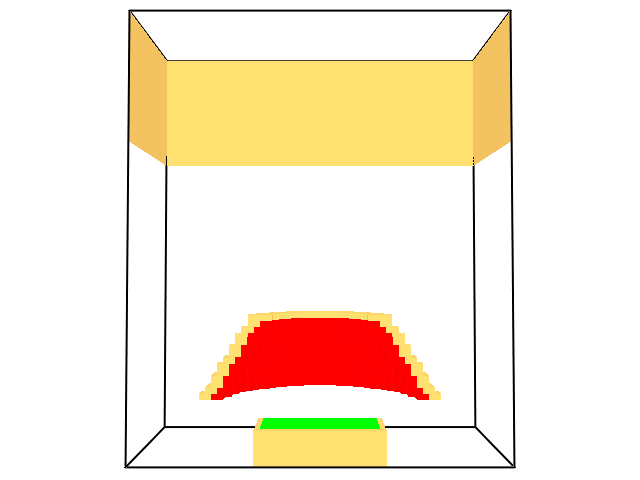
\includegraphics{FIGURES/Spyro_cone_fig}}
        \caption[FDS geometry used for developing the cone reference flux.]{\label{fig:cone_ref_geom} FDS geometry used for developing the cone reference flux. Red is the cone heater and green is the sample surface. The domain is clipped at the plane y=0~m.}
    \end{center}
\end{figure}

A notional fuel molecule was created for each heat of combustion and soot yield that provided an oxygen heat of combustion (EPUMO2) of 13,100~\unit{kJ/kg}. For a 0~\% soot yield, the following was done to obtain fuel chemistry. A heat of combustion of 50~\unit{MJ/kg} implies a fuel like methane and the formula CH$_{3.333}$ provides the desired EPUMO2 at a soot yield of 0~\%. A heat of combustion of 40~\unit{MJ/kg} implies a hydrocarbon like fuel, and the resulting formula is CH$_{0.959}$. For 10, 20 and 30~\unit{MJ/kg} oxygen was added while keeping a C:H ratio of 1:2, resulting in formulas of CH$_{2}$O$_{0.302}$, CH$_{2}$O$_{0.658}$, and CH$_{2}$O$_{1.322}$. The H or O values were varied as needed for the different soot yields to keep an EPUMO2 of 13,100~\unit{kJ/kg}.

If $\dq_{\rm flame}''$ for each heat of combustion is normalized by the maximum value for all HRRPUA, the results collapse as shown in the left of Fig~\ref{fig:Spyro_hoc}. We can then determine a quadratic fit for the maximum $\dq_{\rm flame}''$ as a function of heat of combustion as shown in the right of Fig~\ref{fig:Spyro_hoc}.

\begin{figure}
    \centering
    \begin{tabular*}{\textwidth}{c@{\extracolsep{\fill}}c}
        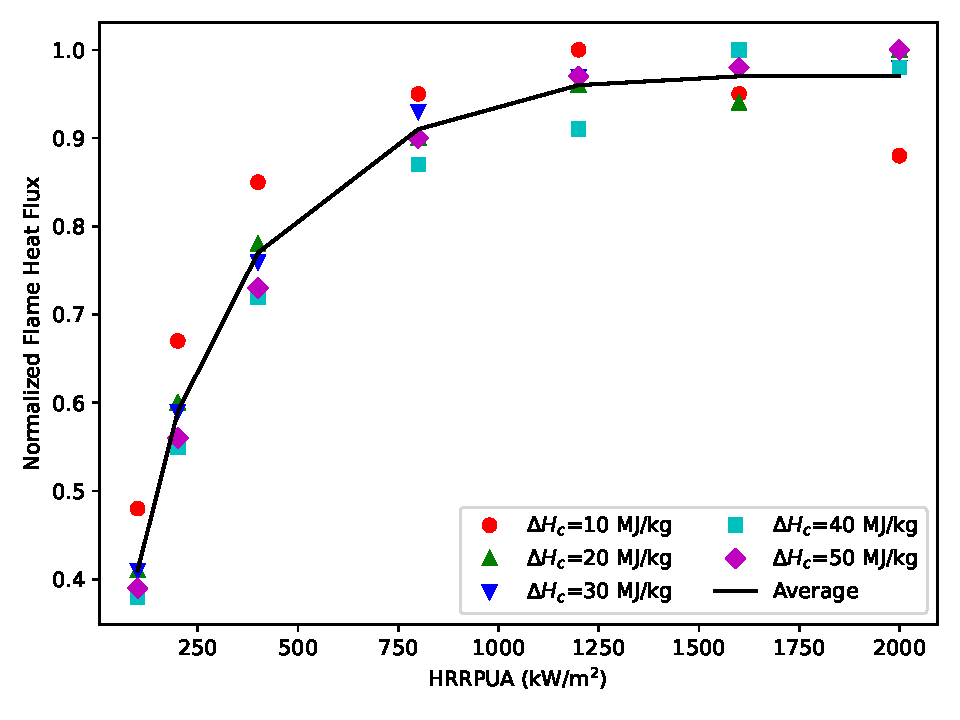
\includegraphics[height=2.2in]{FIGURES/Spyro_hoc_ratio} &
        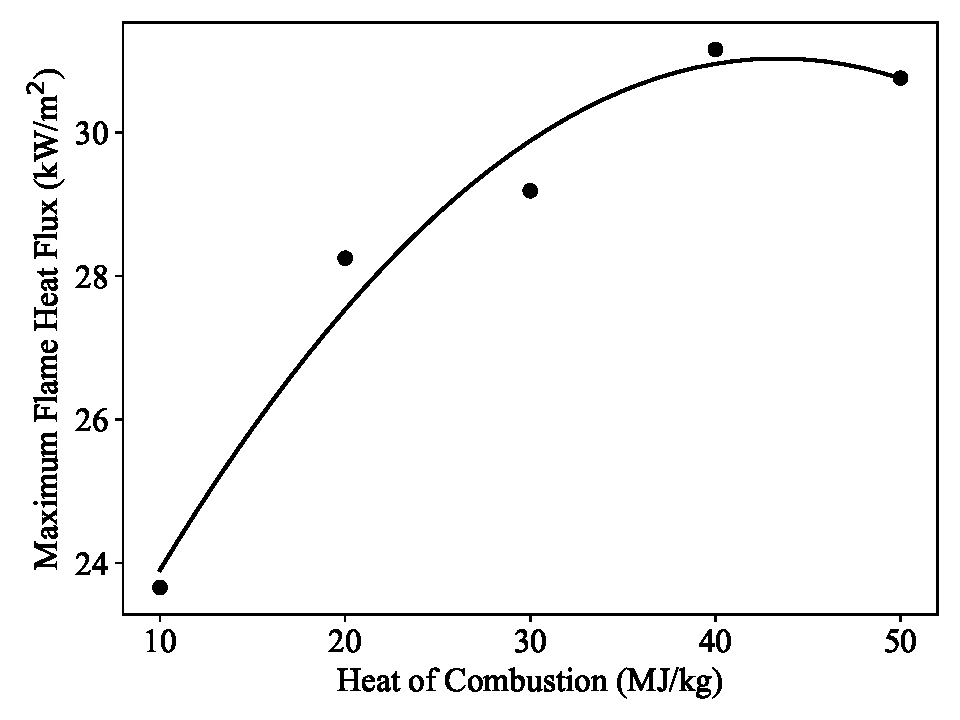
\includegraphics[height=2.2in]{FIGURES/Spyro_hoc_max}
    \end{tabular*}
    \caption[Empirical flame heat flux for Spyro]{(Left) Normalized flame heat flux as a function of HRRPUA. (Right) Maximum flame heat flux as a function of $\Delta h$.}
    \label{fig:Spyro_hoc}
\end{figure}

Various simple combinations of the heat of combustion, soot yield, and HRRPUA were evaluated to determine a relationship for $\Gamma$. The functional form of $A + B \times \hbox{HRRPUA} / \Delta h + C \times \hbox{soot yield}$ gave a fit with the lowest RMS value. To determine the time-dependent $\dq_{\rm ref}''$ for a cone test, first, the maximum $\dq_{\rm flame}''$ is determined using $\Delta h$ at the fit shown in Fig~\ref{fig:Spyro_hoc}, second,  $\dq_{\rm flame}''$ is adjusted for the current HRRPUA by interpolating the average normalized curve in Fig~\ref{fig:Spyro_hoc}, third, $\Gamma$ is determined and used to adjust  $\dq_{\rm cone}''$, and finally, $\dq_{\rm ref}''$ is determined via Eq.~\ref{Spyro7}. The resulting fit has a 2~\% error compared to the FDS predictions, see Fig.~\ref{fig:Spyro_cone_error}.

\begin{figure}[!ht]
\centering
\begin{tabular}{c}
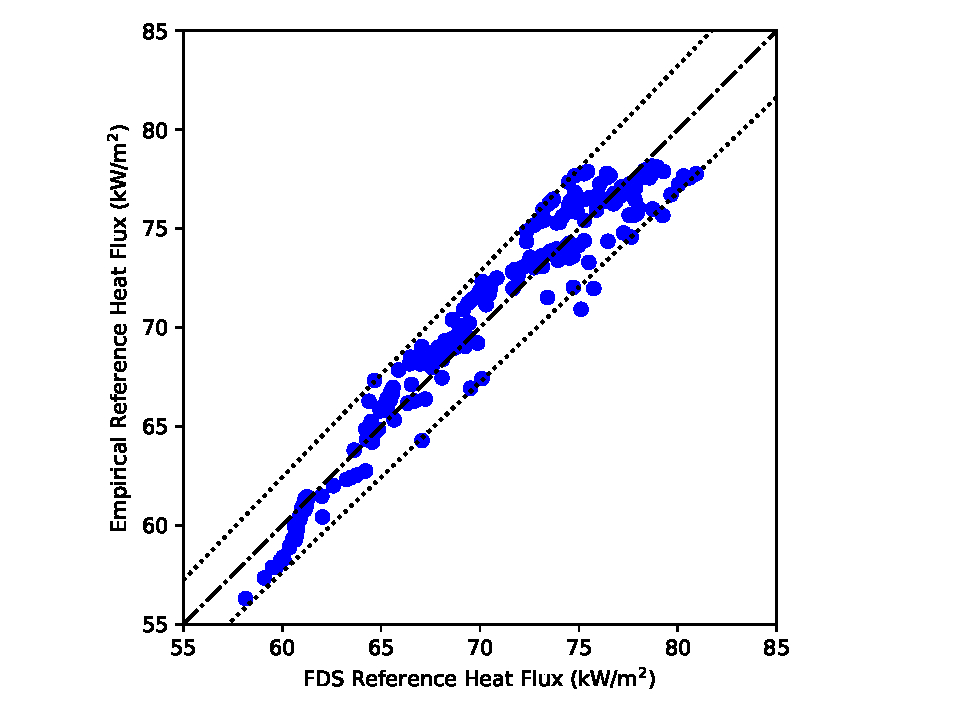
\includegraphics[height=3.5in]{FIGURES/Spyro_cone_error}
\end{tabular}
\caption[Scatterplot for predicted vs. empirical reference heat flux.]{Scatterplot for predicted vs. empirical reference heat flux.}
\label{fig:Spyro_cone_error}
\end{figure}
